%%%%%%%%%%%%%%%%%%%%%%%%%%%%%%%%%%%%%%%%%%%%%%%%%%%%%%%%%%%%%%%%%%%%%%%%%%%%%%%%
% title:
% authors:
%%%%%%%%%%%%%%%%%%%%%%%%%%%%%%%%%%%%%%%%%%%%%%%%%%%%%%%%%%%%%%%%%%%%%%%%%%%%%%%%
\def\fullver{0}
\def\submission{1}
\documentclass[11pt]{article}

\usepackage[letterpaper,hmargin=1in,vmargin=1in]{geometry}
\usepackage[backref=true,backend=bibtex]{biblatex}

\DefineBibliographyStrings{english}{%
  backrefpage = {page},% originally "cited on page"
  backrefpages = {pages},% originally "cited on pages"
}


\usepackage{framed}
%\usepackage{cite}
\usepackage[hidelinks]{hyperref}

\usepackage{color}
\usepackage{float}
\usepackage{setspace}
\usepackage{booktabs}
\usepackage{outlines}
\usepackage{enumitem}
\usepackage{epsfig}
\usepackage{wrapfig}
\usepackage{textcomp}
\usepackage{rotating}
\usepackage{xspace}
\usepackage{tikz}
\usetikzlibrary{calc,arrows,arrows.meta,shapes,positioning,matrix,decorations.pathreplacing}
\usepackage{amsthm}
\usepackage{amssymb}
\usepackage{pifont}
\usepackage{amsfonts}
\usepackage{amsmath}
\DeclareMathOperator*{\argmax}{arg\,max}
\DeclareMathOperator*{\argmin}{arg\,min}
\usepackage{cleveref}
\usepackage{bm}
\usepackage{listings}
\usepackage{mathtools}
\allowdisplaybreaks[2]
\usepackage{latexsym}
\usepackage{graphics}
\usepackage{graphicx}
\usepackage{fancyhdr}
\usepackage{url}
%\usepackage{enumerate}
\usepackage{adjustbox}
\usepackage{multirow}
\usepackage[font=small]{caption}
\usepackage[font=small]{subcaption}
\def\authnotes{1}
\newtheorem{thm}{} %[section]
\newtheorem*{theorem*}{Theorem}
\newtheorem{lem}{Lemma}

\newtheorem{cor}[thm]{Corollary}
\newtheorem{propo}[thm]{Proposition}
\newtheorem{defn}[thm]{Definition}
\newtheorem{assm}[thm]{Assumption}
\newtheorem{clm}[thm]{Claim}
\newtheorem{rem}[thm]{Remark}
\newtheorem{exa}{Example}
\newtheorem{fact}{Fact}

\newenvironment{theorem}{\begin{thm}
    \begin{sl}
    }%
    {
    \end{sl}
  \end{thm}}

\newenvironment{lemma}{\begin{lem}\begin{sl}}%
    {\end{sl}\end{lem}}
\newenvironment{corollary}{\begin{cor}\begin{sl}}%
    {\end{sl}\end{cor}}
\newenvironment{proposition}{\begin{propo}\begin{sl}}%
    {\end{sl}\end{propo}}
\newenvironment{definition}{\begin{defn}\begin{sl}}%
    {\end{sl}\end{defn}}
\newenvironment{assumption}{\begin{assm}\begin{em}}%
    {\end{em}\end{assm}}
\newenvironment{claim}{\begin{clm}\begin{sl}}%
    {\end{sl}\end{clm}}
\newenvironment{remark}{\begin{rem}\begin{em}}%
    {\end{em}\end{rem}}
\newenvironment{example}{\begin{exa}\begin{em}}%
    {\end{em}\end{exa}}

\newcommand{\lemautorefname}{Lemma}
\newcommand{\algorithmautorefname}{Algorithm}
\renewcommand{\subsectionautorefname}{Section}


% Deluxe proof enviroment
\iffalse
    \def\qsym{\vrule width0.6ex height1em depth0ex}
    \def\qedsym{{\hspace{5pt}\rule[-1pt]{3pt}{9pt}}}
    \newcount\proofqeded
    \newcount\proofended
    \def\qed{%\qedsym
    \end{rm}\addtolength{\parskip}{-0pt}
    \setlength{\parindent}{\saveparindent}
    \global\advance\proofqeded by 1 }
    \newenvironment{proof}%
     {\proofstart}%
     {\ifnum\proofqeded=\proofended\qed\fi \global\advance\proofended by 1
      \medskip}
    \makeatletter
    \def\proofstart{\@ifnextchar[{\@oprf}{\@nprf}}
    \def\@oprf[#1]{\begin{rm}\protect\vspace{6pt}\noindent{\bf Proof of #1:\
    }%
    \addtolength{\parskip}{5pt}\setlength{\parindent}{0pt}}
    \def\@nprf{\begin{rm}\protect\vspace{6pt}\noindent{\bf Proof:\ }%
    \addtolength{\parskip}{5pt}\setlength{\parindent}{0pt}}
  \makeatother
\fi


% Extra padding for table entries
\newcommand\Tvsp{\rule{0pt}{2.6ex}}
\newcommand\Bvsp{\rule[-1.2ex]{0pt}{0pt}}
\newcommand{\TabPad}{\hspace*{5pt}}
\newcommand\TabSep{@{\hspace{5pt}}|@{\hspace{5pt}}}
\newcommand\TabSepLeft{|@{\hspace{5pt}}}
\newcommand\TabSepRight{@{\hspace{5pt}}|}



%\def\qedsym{{\ifnum\llncsclass=0  \else {\hspace{5pt}\rule[-1pt]{3pt}{9pt}} \fi}}
\def\qedsym{{\hspace{5pt}\rule[-1pt]{3pt}{9pt}} }

\def\pseudocodesize{ \footnotesize }

\renewcommand{\arraystretch}{1.3}
\DeclareMathAlphabet{\mathsl}{OT1}{cmr}{m}{sl}
\DeclareMathAlphabet{\mathsc}{OT1}{cmr}{m}{sc}


% Reference expansions
\newcommand{\secref}[1]{\mbox{Section~\ref{#1}}}
\newcommand{\subsecref}[1]{\mbox{Subsection~\ref{#1}}}
\newcommand{\apref}[1]{\mbox{Appendix~\ref{#1}}}
\newcommand{\thref}[1]{\mbox{Theorem~\ref{#1}}}
\newcommand{\thmrefshort}[1]{\mbox{\textbf{Th~\ref{#1}}}}
\newcommand{\exref}[1]{\mbox{Example~\ref{#1}}}
\newcommand{\defref}[1]{\mbox{Definition~\ref{#1}}}
\newcommand{\corref}[1]{\mbox{Corollary~\ref{#1}}}
\newcommand{\lemref}[1]{\mbox{Lemma~\ref{#1}}}
\newcommand{\clref}[1]{\mbox{Claim~\ref{#1}}}
\newcommand{\propref}[1]{\mbox{Proposition~\ref{#1}}}
\newcommand{\consref}[1]{\mbox{Construction~\ref{#1}}}
\newcommand{\figref}[1]{\mbox{Figure~\ref{#1}}}
%\newcommand{\eqref}[1]{\mbox{Equation~\ref{#1}}}

\newcommand{\enumref}[1]{\mbox{(\ref{#1})}}

\newcommand{\thmlabel}[1]{\textnormal{\textbf{[#1]}}}

\newcommand{\SetFigFont}[5]{} % This is for xfig issue
\newcommand{\SetFigFontNFSS}[5]{} % This is for xfig issue

\DeclarePairedDelimiter{\ceil}{\lceil}{\rceil}%
\DeclarePairedDelimiter{\floor}{\lfloor}{\rfloor}%
\DeclarePairedDelimiter\absv{\lvert}{\rvert}%
%\DeclarePairedDelimiter\norm{\lVert}{\rVert}%
\DeclarePairedDelimiter\prns{(}{)}%
\DeclarePairedDelimiter\braces{\{}{\}}%
\DeclarePairedDelimiter\bracks{[}{]}%
\DeclarePairedDelimiterX\condprns[2]{(}{)}{\,#1 \;\delimsize\vert\; #2\,}
\DeclarePairedDelimiterX\condbrks[2]{[}{]}{\,#1 \;\delimsize\vert\; #2\,}
\DeclarePairedDelimiterX\condbraces[2]{\{}{\}}{\,#1 \;\delimsize\vert\; #2\,}

% ========================================================================

% Lists

\newcounter{ctr}
\newcounter{savectr}
\newcounter{ectr}

\newlength{\saveparindent}
\setlength{\saveparindent}{\parindent}
\newlength{\saveparskip}
\setlength{\saveparskip}{\parskip}


\newenvironment{newitemize}{%
\begin{list}{\mbox{}\hspace{5pt}$\bullet$\hfill}{\labelwidth=15pt%
\labelsep=5pt \leftmargin=20pt \topsep=3pt%
\setlength{\listparindent}{\saveparindent}%
\setlength{\parsep}{\saveparskip}%
\setlength{\itemsep}{3pt} }}{\end{list}}


\newenvironment{newenum}{%
\begin{list}{{\rm (\arabic{ctr})}\hfill}{\usecounter{ctr} \labelwidth=17pt%
\labelsep=5pt \leftmargin=22pt \topsep=3pt%
\setlength{\listparindent}{\saveparindent}%
\setlength{\parsep}{\saveparskip}%
\setlength{\itemsep}{2pt} }}{\end{list}}

\newenvironment{tiret}{%
\begin{list}{\hspace{2pt}\rule[0.5ex]{6pt}{1pt}\hfill}{\labelwidth=15pt%
\labelsep=3pt \leftmargin=22pt \topsep=3pt%
\setlength{\listparindent}{\saveparindent}%
\setlength{\parsep}{\saveparskip}%
\setlength{\itemsep}{2pt}}}{\end{list}}


\newenvironment{blocklist}{\begin{list}{}{\labelwidth=0pt%
\labelsep=0pt \leftmargin=0pt \topsep=10pt%
\setlength{\listparindent}{\saveparindent}%
\setlength{\parsep}{\saveparskip}%
\setlength{\itemsep}{20pt}}}{\end{list}}

\newenvironment{blocklistindented}{\begin{list}{}{\labelwidth=0pt%
\labelsep=30pt \leftmargin=30pt\topsep=5pt%
\setlength{\listparindent}{\saveparindent}%
\setlength{\parsep}{\saveparskip}%
\setlength{\itemsep}{10pt}}}{\end{list}}

\newenvironment{onelist}{%
\begin{list}{{\rm (\arabic{ctr})}\hfill}{\usecounter{ctr} \labelwidth=18pt%
\labelsep=7pt \leftmargin=25pt \topsep=2pt%
\setlength{\listparindent}{\saveparindent}%
\setlength{\parsep}{\saveparskip}%
\setlength{\itemsep}{2pt} }}{\end{list}}

\newenvironment{twolist}{%
\begin{list}{{\rm (\arabic{ctr}.\arabic{ectr})}%
\hfill}{\usecounter{ectr} \labelwidth=26pt%
\labelsep=7pt \leftmargin=33pt \topsep=2pt%
\setlength{\listparindent}{\saveparindent}%
\setlength{\parsep}{\saveparskip}%
\setlength{\itemsep}{2pt} }}{\end{list}}

\newenvironment{centerlist}{%
\begin{list}{\mbox{}}{\labelwidth=0pt%
\labelsep=0pt \leftmargin=0pt \topsep=10pt%
\setlength{\listparindent}{\saveparindent}%
\setlength{\parsep}{\saveparskip}%
\setlength{\itemsep}{10pt} }}{\end{list}}

\newenvironment{newcenter}[1]{\begin{centerlist}\centering%
\item #1}{\end{centerlist}}

\newenvironment{codecenter}[1]{\begin{small}\begin{centerlist}\centering%
\item #1}{\end{centerlist}\end{small}}

% =========================================================================

% Math

\newlength{\savejot}
\setlength{\jot}{3pt}
\setlength{\savejot}{\jot}

\newenvironment{newmath}{\begin{displaymath}%
\setlength{\abovedisplayskip}{4pt}%
\setlength{\belowdisplayskip}{4pt}%
\setlength{\abovedisplayshortskip}{6pt}%
\setlength{\belowdisplayshortskip}{6pt} }{\end{displaymath}}

\newenvironment{newequation}{\begin{equation}%
\setlength{\abovedisplayskip}{4pt}%
\setlength{\belowdisplayskip}{4pt}%
\setlength{\abovedisplayshortskip}{6pt}%
\setlength{\belowdisplayshortskip}{6pt} }{\end{equation}}

%\newcommand{\headingg}[1]{{\textbf{#1}}}
%\newcommand{\heading}[1]{{\vspace{6pt}\noindent\textbf{#1}}}
\newcommand{\ind}{\hspace*{1.5em}}
\newcommand{\indsm}{\hspace*{.75em}}
\newcommand{\indeqn}{\;\;\;\;\;\;\;}
\newcommand{\bits}{\{0,1\}}
\newcommand{\zon}[1]{\bits^{#1}}
\newcommand{\emptystring}{\varepsilon}
\newcommand{\xor}{{\:\oplus\:}}
%\newcommand{\concat}{\,,\,}
\newcommand{\smidge}{{\kern .05em}}
\newcommand{\Colon}{{\smidge\colon\smidge}}
\newcommand{\norm}[1]{\|#1\|}
\def\poly{\mathop{\rm poly}\nolimits}
\def\div{\mathop{\rm div}\nolimits}
%\newcommand{\ro}{RO}
\newcommand{\advA}{{\mathcal A}}
\newcommand{\advB}{{\mathcal B}}
\newcommand{\advC}{{\mathcal C}}
\newcommand{\advD}{{\mathcal D}}
\newcommand{\advE}{{\mathcal E}}

\newcommand{\calA}{{\cal A}}
\newcommand{\calB}{{\cal B}}
\newcommand{\calC}{{\cal C}}
\newcommand{\calE}{{\cal E}}
\newcommand{\calF}{{\cal F}}
\newcommand{\calG}{{\cal G}}
\newcommand{\calH}{{\cal H}}
\newcommand{\calI}{{\cal I}}
\newcommand{\calJ}{{\cal J}}
\newcommand{\calO}{{\cal O}}
\newcommand{\calR}{{\cal R}}
\newcommand{\calS}{{\cal S}}
\newcommand{\calD}{{\cal D}}
\newcommand{\calK}{{\cal K}}
\newcommand{\calL}{{\cal L}}
\newcommand{\calM}{{\cal M}}
\newcommand{\calN}{{\cal N}}
\newcommand{\calP}{{\cal P}}
\newcommand{\calQ}{{\cal Q}}
\newcommand{\calT}{{\cal T}}
\newcommand{\calU}{{\cal U}}
\newcommand{\calV}{{\cal V}}
\newcommand{\calW}{{\cal W}}
\newcommand{\calX}{{\cal X}}
\newcommand{\calY}{{\cal Y}}

\newcommand{\N}{{{\mathbb N}}}
\newcommand{\Z}{{{\mathbb Z}}}
\newcommand{\G}{{{\textnormal G}}}
\newcommand{\Hgame}{{{\textnormal H}}}
\newcommand{\bigO}{\calO}
\newcommand{\goesto}{{\rightarrow}}
\newcommand{\eqdef}{\stackrel{\rm def}{=}}
\newcommand{\negsmidge}{{\hspace{-0.1ex}}}
\newcommand{\cdotsm}{\negsmidge\negsmidge\negsmidge\cdot\negsmidge\negsmidge\negsmidge}
\def\union{\cup}
\def\sep{\,}
\def\bigunion{\bigcup}
\def\suchthatt{\: :\:}
%\def\next{\hspace{12pt};\hspace{12pt}}
\def\nextt{\hspace{3pt};\hspace{6pt}}
\newcommand{\set}[2]{\{\:#1 \suchthatt #2\:\}}
\newcommand{\card}[1]{|#1|}
\def\leqq{\;\leq\;}
\def\eqq{\;=\;}
\def\geqq{\;\geq\;}
\def\lst{\;<\;}
\def\gst{\;>\;}
\def\prn#1{\left(#1\right)}

% \newcolumntype{y}[1]{%
% >{\hspace{0pt}}p{#1}}%

% \newcolumntype{x}[1]{%
% >{\centering\hspace{0pt}}p{#1}}%




\newcommand{\verylongleftarrow}[1]
      {\setlength{\unitlength}{.01in}
      \begin{picture}(#1,1) \put(#1,0){\vector(-1,0){#1}} \end{picture}}
\newcommand{\verylongrightarrow}[1]             %longleft and rightgoing arrows
      {\setlength{\unitlength}{.01in}           %for protocols
      \begin{picture}(#1,1) \put(0,0){\vector(1,0){#1}} \end{picture}}
\newcommand{\verylongbotharrow}[2]             %longleft and rightgoing arrows
      {\setlength{\unitlength}{.01in}           %for protocols
      \begin{picture}(#2,1) \put(#1,0){\vector(1,0){#1}}
                            \put(#1,0){\vector(-1,0){#1}} \end{picture}}
\newcommand{\leftgoing}[2]{{\stackrel{{\displaystyle #2}} {\verylongleftarrow{#1}}}}
\newcommand{\rightgoing}[2]{{\stackrel{{\displaystyle #2}} {\verylongrightarrow{#1}}}}
\newcommand{\bothgoing}[3]{{\stackrel{{\displaystyle #3}} {\verylongbotharrow{#1}{#2}}}}


\newcommand{\leftgoinga}[1]{\leftgoing{230}{#1} }
\newcommand{\rightgoinga}[1]{\rightgoing{230}{#1} }

\newcommand{\leftgoingb}[1]{\leftgoing{300}{#1} }
\newcommand{\rightgoingb}[1]{\rightgoing{300}{#1} }




\newcommand{\veryshortleftarrow}[1]
      {\setlength{\unitlength}{.01in}
      \begin{picture}(#1,1) \put(#1,0){\vector(-1,0){#1}} \end{picture}}


\newcommand{\getparse}[1]{{\:\stackrel{\raisebox{-0.5em}{{\hspace{0.1em}\mbox{\boldmath$\scriptscriptstyle
            #1$}}}}{\leftarrow}\:}}
\newcommand{\getu}{{\:\stackrel{\raisebox{-0.5em}{{\hspace{0.1em}\mbox{\boldmath$\scriptscriptstyle \cup$}}}}{\leftarrow}\:}}
\newcommand{\getdiff}{{\:\stackrel{{\scriptscriptstyle\hspace{0.2em} /}}{\leftarrow}\:}}
\newcommand{\getsr}{{\:{\leftarrow{\hspace*{-3pt}\raisebox{.75pt}{$\scriptscriptstyle\$$}}}\:}}
\newcommand{\get}[1]{{\:\leftarrow_{#1}\:}}
%\newcommand{\getsr}{{\:{\raisebox{3pt}{\veryshortleftarrow{15}}{\raisebox{1pt}{$\scriptscriptstyle\$$}}}\:}}
%\newcommand{\getsr}{{\:{\xleftarrow{\scriptscriptstyle\$}}\:}}
%\newcommand{\getsr}{{\:\stackrel{\raisebox{-0.5em}{$\scriptscriptstyle \hspace{0.2em}\$$}}{\leftarrow}\:}}
\newcommand{\sendsr}{{\:\stackrel{\scriptscriptstyle \hspace{0.2em}\$}{\rightarrow}\:}}
\renewcommand{\choose}[2]{{{#1}\atopwithdelims(){#2}}}
\newcommand{\abs}[1]{{\displaystyle \left| {#1} \right| }}
\newcommand{\E}{{\mbox{\bf E}}}
\newcommand{\EE}[1]{{\E\left[{#1}\right]}}
\newcommand{\EEE}[2]{{\E_{#1}\left[{#2}\right]}}
\newcommand{\Ex}{{\textbf E}}
\newcommand{\Exx}[1]{{\Ex\left[{#1}\right]}}
\newcommand{\Exxx}[2]{{\Ex_{#1}\left[{#2}\right]}}
\newcommand{\Var}{{\textnormal{Var}}}
\newcommand{\Varr}[1]{{\Var\left[{#1}\right]}}
\newcommand{\Varrr}[2]{{\Var_{#1}\left[{#2}\right]}}
\newcommand{\Prob}[1]{\Pr\left[\: #1 \:\right]}
\newcommand{\CondProb}[2]{{\Pr}\left[\: #1\:\left|\right.\:#2\:\right]}
\newcommand{\CondProbb}[3]{{\Pr}_{#1}\left[\: #2\:\left|\right.\:#3\:\right]}
\newcommand{\ProbExp}[2]{\Pr\left[\: #1 \: : \: #2\: \right]}
\newcommand{\Probb}[2]{{\Pr}_{#1}\left[\: #2 \:\right]}
\newcommand{\Probc}[2]{\Pr\left[\: #1 \:{\left|\right.}\:#2\:\right]}
\newcommand{\Probcc}[3]{{\Pr}_{#1}\left[\: #2 \:\left|\right.\:#3\:\right]}
\newcommand{\suchthat}{{\mbox{s.t.\ }}}
\newcommand{\qquadd}{{\quad}}
\def\d{{\delta}}
\def\e{{\epsilon}}
\newcommand{\ceiling}[1]{\lceil #1\rceil}
\newcommand{\sfrac}[2]{{\textstyle \frac{#1}{#2}}}
\newcommand{\ssum}[2]{{\textstyle \sum_{\,#1}^{\,#2}\,}}
\newcommand{\sprod}[2]{{\textstyle \prod_{\,#1}^{\,#2}\,}}
\def\smax{{\textstyle \max}}
%\def\N{{\sf N}}
\def\R{{\sf R}}
%\def\getsr{\stackrel{\$}{\leftarrow}}
\newcommand{\blockindex}[2]{{\langle#1\rangle}_{#2}}
\def\chv{\raisebox{2pt}{$\chi$}}

\newcommand{\cclass}[1]{{\rm #1}}
\def\P{\cclass{P}}
\def\NP{\cclass{NP}}
\def\BPP{\cclass{BPP}}
\def\coRP{\cclass{coRP}}
\def\NEXP{\cclass{NEXP}}
\def\DES{\mbox{\rm DES}}
\newcommand{\md}{\textsf{md5}}
\newcommand{\MD}{\textnormal{MD}}
\newcommand{\MDb}{\textbf{MD}}
\newcommand{\sha}{\textsf{sha-1}}
\newcommand{\ripemd}{\textsf{ripemd-160}}

\newcommand{\badSet}{\calS}
\newcommand{\bad}{\ensuremath{\mathsf{bad}}}
\newcommand{\cbad}{\bad}
\newcommand{\ctrue}{\true}
\newcommand{\notbad}{\overline{\bad}}
\newcommand{\win}{\ensuremath{\mathsf{win}}}
\newcommand{\outputs}{\:{\Rightarrow}\:}
\newcommand{\cheat}{\mathsf{cheat}}
\newcommand{\cheattrue}{\cheat\gets\true}
\newcommand{\notcheated}{\mathsf{Honest}}
\newcommand{\badtrue}{\bad\gets\true}
\newcommand{\Good}{\mathsf{Good}}
\newcommand{\good}{\mathsf{good}}
\newcommand{\EvNbadA}{\overline{\mathsf{Bad}}_1}
\newcommand{\EvbadA}{\mathsf{Bad}_1}
\newcommand{\EvNbadB}{\overline{\mathsf{Bad}}_2}
\newcommand{\EvbadB}{\mathsf{Bad}_2}
\newcommand{\badA}{\bad_1}
\newcommand{\badB}{\bad_2}
\newcommand{\badC}{\bad_3}
\newcommand{\badAtrue}{\badA\gets\true}
\newcommand{\badBtrue}{\badB\gets\true}
\newcommand{\badCtrue}{\badC\gets\true}
\newcommand{\setsbad}{\mbox{~\textup{sets} $\bad$}\,}
\newcommand{\setsbadA}{\mbox{~\textup{sets} $\badA$}\,}
\newcommand{\setsbadB}{\mbox{~\textup{sets} $\badB$}\,}
\newcommand{\setsbadzero}{\mbox{~\textup{sets} $\badzero$}\,}
\newcommand{\setsbadone}{\mbox{~\textup{sets} $\badone$}\,}
\newcommand{\setsbadtwo}{\mbox{~\textup{sets} $\badtwo$}\,}
\newcommand{\setsbadthree}{\mbox{~\textup{sets} $\badthree$}\,}
\newcommand{\setsbadfour}{\mbox{~\textup{sets} $\badfour$}\,}
\newcommand{\badzero}{\ensuremath{\mathsf{bad}_0}}
\newcommand{\badone}{\ensuremath{\mathsf{bad}_1}}
\newcommand{\badtwo}{\ensuremath{\mathsf{bad}_2}}
\newcommand{\badthree}{\ensuremath{\mathsf{bad}_3}}
\newcommand{\badfour}{\ensuremath{\mathsf{bad}_4}}
\newcommand{\defined}{\ensuremath{\mathsf{defined}}}
%\newcommand{\undefined}{\ensuremath{\mathsf{undefined}}}
\newcommand{\true}{\ensuremath{\mathsf{true}}}
\newcommand{\false}{\ensuremath{\mathsf{false}}}
\newcommand{\zero}{\ensuremath{\mathsf{zer}}}
\newcommand{\one}{\ensuremath{\mathsf{one}}}
\newcommand{\Initialize}{{\textbf{Initialize}}}
\newcommand{\Finalize}  {{\textbf{Finalize}}}
\newcommand{\Onquery}   {{\textbf{procedure~}}}
\newcommand{\onquery}   {{\textbf{query~}}}
\newcommand{\Update}{{\textnormal{update}}}
%\newcommand{\algorithm}[1]{{\textbf{algorithm~}{#1}}}
\newcommand{\fn}{\footnotesize}

\newcommand{\hash}{\mathcal{H}}

\newcommand{\Hash}{\textbf{Hash}}
\newcommand{\fEval}{\textbf{f-Eval}}
\newcommand{\fReveal}{\textbf{f-Reveal}}

\newcommand{\xRV}{X_{t,i}}
\newcommand{\XRV}{X_t}
\newcommand{\zRV}{Z_{t\concat r}}
\newcommand{\ZRV}{Z}
\newcommand{\const}{\mathsf{c}}

% from /usr/local/lib/TeX+MF/tex/macros/art11.sty

\makeatletter

\def\subsubsection{\@startsection{subsubsection}{3}{\z@}{-2.25ex plus
 -1ex minus -.2ex}{1.5ex plus .2ex}{\sf}}


% =========================================================================


% Definitions for this paper
\newcommand{\secparam}{\kappa}
\newcommand{\ctr}{\mathit{ctr}}
\newcommand{\MAC}{\mathsf{MAC}}
\newcommand{\kwfont}[1]{\textrm{#1}}
\newcommand{\procfont}[1]{\textbf{#1}}
\newcommand{\nfont}[1]{{\footnotesize #1}}
\newcommand{\lnum}[1]{{\footnotesize #1}\;\;}

\newcommand{\ETS}[2]{\cal{ETS}_{#1}^{#2}}

\newcommand{\Exp}{\mathbf{Exp}}
\newcommand{\MUExp}[4]{\mathbf{Exp}^{\mathrm{n \mbox{-}mu\mbox{-}#4\mbox{-}#1}}_{#2}(#3)}
%\newcommand{\SUExp}[2]{\mathbf{Exp}^{\mathrm{su\mbox{-}cpa\mbox{-}#2}}_{#1}}
\newcommand{\SUExp}[3]{\mathbf{Exp}^{\mathrm{ind\mbox{-}{#3}}}_{#1}(#2)}
\newcommand{\ForgeExp}[2]{\mathbf{Exp}^{\mathrm{uf\mbox{-}cma}}_{#1}(#2)}
\newcommand{\LeakExp}[3]{\mathbf{Exp}^{\mathrm{pred\mbox{-}ct\mbox{-}#3}}_{#1}(#2)}
\newcommand{\CompExp}[3]{\mathbf{Exp}^{\mathrm{pred\mbox{-}pt\mbox{-}#3}}_{#1}(#2)}
\newcommand{\FuncExp}[2]{\mathbf{Exp}^{\mathrm{ss\mbox{-}real}}_{#1}(#2)}
\newcommand{\FuncExpReal}[2]{\mathbf{Exp}^{\mathrm{ror\mbox{-}det\mbox{-}real}}_{#1}(#2)}
\newcommand{\FuncExpRand}[2]{\mathbf{Exp}^{\mathrm{ror\mbox{-}det\mbox{-}rand}}_{#1}(#2)}
\newcommand{\FuncExpRealH}[2]{\mathbf{Exp}^{\mathrm{hyb\mbox{-}det\mbox{-}real}}_{#1}(#2)}
\newcommand{\FuncExpRandH}[2]{\mathbf{Exp}^{\mathrm{hyb\mbox{-}det\mbox{-}rand}}_{#1}(#2)}
\newcommand{\FuncExpD}[2]{\mathbf{Exp}^{\mathrm{det\mbox{-}1}}_{#1}(#2)}
\newcommand{\FuncExpS}[3]{\mathbf{Exp}^{\mathrm{priv\mathrm{\mbox{-}#3}\mbox{-}1}}_{#1}(#2)}
\newcommand{\FuncExpDR}[2]{\mathbf{Exp}^{\mathrm{ss\mbox{-}det\mbox{-}rand}}_{#1}(#2)}
\newcommand{\FuncPTExp}[2]{\mathbf{Exp}^{\mathrm{func\mbox{-}pt}}_{#1}(#2)}
\newcommand{\PlainFuncExp}[3]{\mathbf{Exp}^{\mathrm{func\mbox{-}nil\mbox{-}#3}}_{#1}(#2)}
\newcommand{\FuncPredExp}[2]{\mathbf{Exp}^{\mathrm{ss\mbox{-}sim}}_{#1}(#2)}
\newcommand{\FuncPredExpD}[2]{\mathbf{Exp}^{\mathrm{det\mbox{-}0}}_{#1}(#2)}
\newcommand{\FuncPredExpS}[3]{\mathbf{Exp}^{\mathrm{priv\mathrm{\mbox{-}#3}\mbox{-}0}}_{#1}(#2)}
\newcommand{\SSExp}[2]{\mathbf{Exp}^{\mathrm{ss}\mbox{-}\mathrm{real}}_{#1}(#2)}
\newcommand{\SSExpS}[2]{\mathbf{Exp}^{\mathrm{ss\mbox{-}sim}}_{#1}(#2)}
\newcommand{\InvertExp}[2]{\mathbf{Exp}^{\mathrm{pt\mbox{-}pred}}_{#1}(#2)}
\newcommand{\IndOracle}[2]{\mathbf{I}_{#1}(#2)}
\newcommand{\BOracle}{\mathsf{B}}
\newcommand{\EqOracle}{\mathsf{Eq}}
\newcommand{\REC}{\mathsf{REC}}
\newcommand{\notask}{\overline{\mathsc{Ask}}}
\newcommand{\ask}{\mathsc{Ask}}
\newcommand{\MQ}{\mathsf{MsgQueried}}
\newcommand{\MG}{\mathsf{QueryOfMsgGuessed}}
\newcommand{\MC}{\mathsf{MsgChosenAgain}}
\newcommand{\MT}{\mathsf{MsgTargeted}}
\newcommand{\AT}{\mathsf{AdvFindsTarget}}
\newcommand{\ME}{\mathsf{MsgsAreEqual}}
\newcommand{\QM}{\mathsf{AskM}}
\newcommand{\QR}{\mathsf{AskM_r}}
\newcommand{\TG}{\mathsf{CorrGuess}}
\newcommand{\flips}{n_{\text{f}}}
\newcommand{\mprime}{m^{\prime}}

\newcommand{\queries}{q}

\newcommand{\Aguess}{A_{\mathrm{g}}}
\newcommand{\Ad}{A_{\mathrm{d}}}
\newcommand{\Ap}{A_{\mathrm{p}}}
\newcommand{\Af}{A_{\mathrm{f}}}
\newcommand{\Ag}{A_{\mathrm{g}}}
\newcommand{\Am}{A_{\mathrm{m}}}
\newcommand{\Ac}{A_{\mathrm{c}}}
\newcommand{\Ai}{A_{\mathrm{i}}}



\newcommand{\Aone}{A_1}
\newcommand{\Atwo}{A_2}
\newcommand{\Done}{D_1}
\newcommand{\Dtwo}{D_2}

\newcommand{\Agone}{A^*_{\mathrm{g}}}
\newcommand{\Amone}{A^*_{\mathrm{m}}}
\newcommand{\Acone}{A^*_{\mathrm{c}}}

\newcommand{\Astar}{A^*}
\newcommand{\Agstar}{A^*_{\mathrm{g}}}
\newcommand{\Amstar}{A^*_{\mathrm{m}}}
\newcommand{\Acstar}{A^*_{\mathrm{c}}}

\newcommand{\Ig}{I_{\mathrm{g}}}
\newcommand{\Iguess}{\Ig}
\newcommand{\Imsg}{I_{\mathrm{m}}}
\newcommand{\Ic}{I_{\mathrm{c}}}
\newcommand{\Ip}{I_{\mathrm{p}}}
\newcommand{\Is}{I_{\mathrm{s}}}

\newcommand{\Istar}{I^*}
\newcommand{\Igstar}{I^*_{\mathrm{g}}}
\newcommand{\Imstar}{I^*_{\mathrm{m}}}
\newcommand{\Icstar}{I^*_{\mathrm{c}}}


\newcommand{\Jm}{J_{\mathrm{m}}}
\newcommand{\Jg}{J_{\mathrm{g}}}
\newcommand{\Jc}{J_{\mathrm{c}}}
\newcommand{\Jp}{J_{\mathrm{p}}}
\newcommand{\Js}{J_{\mathrm{s}}}

\newcommand{\Dm}{D_{\mathrm{m}}}
\newcommand{\Dc}{D_{\mathrm{c}}}
\newcommand{\Dp}{D_{\mathrm{p}}}
\newcommand{\Dg}{D_{\mathrm{g}}}

\newcommand{\Pg}{P_{\mathrm{g}}}
\newcommand{\Pp}{P_{\mathrm{p}}}
\newcommand{\Pt}{P_{\mathrm{t}}}
\newcommand{\Pguess}{\Pg}
\newcommand{\Pmsg}{P_{\mathrm{m}}}
\newcommand{\Pm}{\Pmsg}
\newcommand{\Pc}{P_{\mathrm{c}}}
\newcommand{\Pd}{P_{\mathrm{d}}}


\newcommand{\Bc}{B_{\mathrm{c}}}
\newcommand{\Bf}{B_{\mathrm{f}}}
\newcommand{\Bg}{B_{\mathrm{g}}}
\newcommand{\Bm}{B_{\mathrm{m}}}
\newcommand{\Bi}{B_{\mathrm{i}}}

\newcommand{\SSAdv}{\calA_{\mathrm{SS}}}
\newcommand{\TrivAdv}{\calA_\emptystr}
%\newcommand{\LegAdv}{\calA_L}
%\newcommand{\EQAdv}{\calA_{\mathrm{E}}}
\newcommand{\BoolAdv}{\calA_{\mathrm{B}}}
\newcommand{\BBAdv}{\calA_{\mathrm{BB}}^\delta}
\newcommand{\MEAdv}{\calA_{\mathrm{ME}}^\mu}
\newcommand{\UMEAdv}{\calA_{\mathrm{UN}}}
\newcommand{\IMAdv}{\calA_{\times}}
\newcommand{\AdvSep}{\calA_{\mathrm{sep}}}

\newcommand{\AdvJell}{\calJ_{\ell}}
\newcommand{\AdvJzero}{\calJ_{0}}
\newcommand{\AdvIell}{\calJ_{\ell}}
\newcommand{\AdvDell}{\calD_{\ell}}

\newcommand{\AdvJme}{\calJ_{\mathrm{ME}}^\mu}
\newcommand{\AdvDme}{\calD_{\mathrm{ME}}^\mu}

\newcommand{\MEAdvv}[1]{\calA_{\mathrm{E}}^{#1}}
\newcommand{\HEAdv}{\calA_{\mathrm{HE}}}
\newcommand{\SMEAdv}{\calA_{\mathrm{SME}}^\mu}

\newcommand{\INDCPA}{\textnormal{IND-CPA}\xspace}
\newcommand{\INDCCA}{\textnormal{IND-CCA}\xspace}
\newcommand{\INDRAND}{\textnormal{IND\$}\xspace}
\newcommand{\INDSIM}{\textnormal{IND-SIM}\xspace}

\newcommand{\INDAdv}{\calI}
\newcommand{\TrivAdvI}{\calI_\emptystr}
\newcommand{\MEAdvI}{\calI_{\mathrm{ME}}^\mu}
\newcommand{\MEAdvvI}[1]{\calI_{\mathrm{ME}}^{#1}}
\newcommand{\HEAdvI}{\calI_{\mathrm{HE}}}
\newcommand{\SMEAdvI}{\calI_{\mathrm{SME}}^\mu}

\newcommand{\setZero}{\mathtt{I}_0}

%\newcommand{\MUExpcca}[2]{\mathbf{Exp}^{\mathrm{n \mbox{-}mu\mbox{-}cca\mbox{-}#2}}_{#1}}
%\newcommand{\SUExpcca}[2]{\mathbf{Exp}^{\mathrm{su\mbox{-}cca}\mbox{-}{#2}}_{#1}}
\newcommand{\DDHRealexp}[2]{\mathbf{Exp}^{\mathrm{ddh\mbox{-}real}}_{#1}(#2)}
\newcommand{\DDHRandexp}[2]{\mathbf{Exp}^{\mathrm{ddh\mbox{-}rand}}_{#1}(#2)}

\newcommand{\HyExp}{\mathbf{ExpH}}
\newcommand{\find}{\mathsf{find}}
\newcommand{\guess}{g}

\newcommand{\wPRF}{\mathsf{wPRF}}

\newcommand{\Succ}{\mathsf{Succ}}
\newcommand{\Adv}{\mathbf{Adv}}
\newcommand{\Advcpa}[1]{\Adv^{\mathrm{ind\mbox{-}cpa}}_{#1}}
\newcommand{\Advcca}[1]{\Adv^{\mathrm{ind\mbox{-}cca}}_{#1}}
\newcommand{\AdvBIND}[2]{\Adv^{\mathrm{r\dash bind}}_{#1}(#2)}
\newcommand{\AdvRBIND}[2]{\Adv^{\mathrm{r\dash bind}}_{#1}(#2)}
\newcommand{\AdvSRBIND}[2]{\Adv^{\mathrm{sr\dash bind}}_{#1}(#2)}

\newcommand{\AdvVFROB}[2]{\Adv^{\mathrm{efrob}}_{#1}(#2)}
\newcommand{\AdvSBIND}[2]{\Adv^{\mathrm{s\dash bind}}_{#1}(#2)}
\newcommand{\AdvDBIND}[2]{\Adv^{\mathrm{t\dash bind}}_{#1}(#2)}
\newcommand{\AdvMRBIND}[2]{\Adv^{\mathrm{mr\dash bind}}_{#1}(#2)}
\newcommand{\AdvVBIND}[2]{\Adv^{\mathrm{v\dash bind}}_{#1}(#2)}
\newcommand{\AdvNAE}[1]{\Adv^{\mathrm{dae}}_{#1}}
\newcommand{\AdvFROB}[2]{\Adv^{\mathrm{frob}}_{#1}(#2)}
\newcommand{\AdvOTROR}[2]{\Adv^{\mathrm{ot \dash ror}}_{#1}(#2)}
\newcommand{\AdvOTCTXT}[2]{\Adv^{\mathrm{scu}}_{#1}(#2)}
\newcommand{\AdvotCTXT}[2]{\Adv^{\mathrm{ot-ctxt}}_{#1}(#2)}
\newcommand{\AdvTBC}[2]{\Adv^{\mathrm{t\dash sprp}}_{#1}(#2)}

\newcommand{\AdvMEANBIND}[1]{\Adv^{\mathrm{mbind}}_{#1}}
\newcommand{\Coins}{\mathsf{Coins}}
\newcommand{\inv}{^{-1}}
 \newcommand{\AdvPOW}[2]{\Adv^{\mathrm{pow}}_{#1}(#2)}
 \newcommand{\ExpPOW}[2]{\mathbf{Exp}^{\mathrm{pow}}_{#1}(#2)}
 \newcommand{\ExpPOWW}[3]{\mathbf{Exp}^{\mathrm{pow\mbox{-}#2}}_{#1}(#3)}

 \newcommand{\AdvPRIV}[2]{\Adv^{\mathrm{priv}}_{#1}(#2)}
 \newcommand{\ExpPRIV}[2]{\mathbf{Exp}^{\mathrm{priv}}_{#1}(#2)}
 \newcommand{\ExpPRIVV}[3]{\mathbf{Exp}^{\mathrm{priv\mbox{-}#2}}_{#1}(#3)}

 \newcommand{\XCSS}{\textnormal{X-CSS}\xspace}
 \newcommand{\XSSS}{\textnormal{X-SSS}\xspace}
 \newcommand{\CSS}{\textnormal{CSS}\xspace}
 \newcommand{\FCSS}{\textnormal{A-CSS}\xspace}
 \newcommand{\BCSS}{\textnormal{B-CSS}\xspace}
 \newcommand{\BBCSS}{\textnormal{BB-CSS}\xspace}
 \newcommand{\BBCSSbf}{\textbf{BBCSS}\xspace}
 \newcommand{\CSSbf}{\textbf{CSS}\xspace}
 \newcommand{\AdvCSS}[2]{\Adv^{\mathrm{css}}_{#1}(#2)}
 \newcommand{\AdvBBCSS}[2]{\Adv^{\mathrm{bbcss}}_{#1}(#2)}
 \newcommand{\ExpCSS}[2]{\mathbf{Exp}^{\mathrm{css}}_{#1}(#2)}
 \newcommand{\ExpCSSS}[3]{\mathbf{Exp}^{\mathrm{css\mbox{-}#2}}_{#1}(#3)}

 \newcommand{\SSS}{\textnormal{SSS}\xspace}
 \newcommand{\SSSbf}{\textbf{SSS}\xspace}
 \newcommand{\FSSS}{\textnormal{A-SSS}\xspace}
 \newcommand{\BSSS}{\textnormal{B-SSS}\xspace}
 \newcommand{\BBSSS}{\textnormal{BB-SSS}\xspace}
 \newcommand{\BBSSSbf}{\textbf{BBSSS}\xspace}
 \newcommand{\AdvSSS}[2]{\Adv^{\mathrm{sss}}_{#1}(#2)}
 \newcommand{\ExpSSS}[2]{\mathbf{Exp}^{\mathrm{sss}}_{#1}(#2)}
 \newcommand{\ExpSSSS}[3]{\mathbf{Exp}^{\mathrm{sss\mbox{-}#2}}_{#1}(#3)}
 \newcommand{\prf}{F}
 \newcommand{\dash}{\mbox{-}}
 \newcommand{\IND}{\textnormal{IND}\xspace}
 \newcommand{\INDbf}{\textbf{IND}\xspace}
 \newcommand{\ExpSPRP}[2]{\mathbf{Exp}^{\mathrm{sprp}}_{#1}(#2)}
\newcommand{\AdvPRPprime}[2]{\Adv^{\mathrm{prp'}}_{#1}(#2)}
 \newcommand{\ExpPRPprime}[2]{\mathbf{Exp}^{\mathrm{prp'}}_{#1}(#2)}
 \newcommand{\AdvNPRG}[2]{\Adv^{\mathrm{prg}}_{#1}(#2)}
 %\newcommand{\AdvOTPRF}[2]{\Adv^{\mathrm{ot\dash prf}}_{#1}(#2)}
 \newcommand{\AdvMUPRF}[2]{\Adv^{\mathrm{mu\dash prf}}_{#1}(#2)}
 \newcommand{\ExpPRF}[2]{\mathbf{Exp}^{\mathrm{prf}}_{#1}(#2)}
 \newcommand{\AdvIND}[2]{\Adv^{\mathrm{ind}}_{#1}(#2)}
 \newcommand{\AdvINDCCA}[2]{\Adv^{\mathrm{ind\dash cca}}_{#1}(#2)}
 \newcommand{\ExpIND}[2]{\mathbf{Exp}^{\mathrm{ind}}_{#1}(#2)}
 \newcommand{\ExpINDD}[3]{\mathbf{Exp}^{\mathrm{ind\dash#2}}_{#1}(#3)}
 \newcommand{\ExpINDCCA}[2]{\mathbf{Exp}^{\mathrm{ind\dash cca}}_{#1}(#2)}
 \newcommand{\ExpINDCCAD}[3]{\mathbf{Exp}^{\mathrm{ind\dash cca\dash#2}}_{#1}(#3)}

 \newcommand{\AdvKEMCCA}[2]{\Adv^{\mathrm{kem\dash cca}}_{#1}(#2)}
 \newcommand{\AdvKEMCPA}[2]{\Adv^{\mathrm{kem}}_{#1}(#2)}
 \newcommand{\ExpKEMCCA}[2]{\mathbf{Exp}^{\mathrm{kem\dash cca}}_{#1}(#2)}
 \newcommand{\ExpKEMCPA}[2]{\mathbf{Exp}^{\mathrm{kem}}_{#1}(#2)}

 \newcommand{\AdvLOR}[2]{\Adv^{\mathrm{lor}}_{#1}(#2)}
 \newcommand{\AdvLORCCA}[2]{\Adv^{\mathrm{lor\dash cca}}_{#1}(#2)}
 \newcommand{\ExpLOR}[2]{\mathbf{Exp}^{\mathrm{lor}}_{#1}(#2)}
 \newcommand{\ExpLORCCA}[2]{\mathbf{Exp}^{\mathrm{lor\dash cca}}_{#1}(#2)}
 \newcommand{\Enc}{\procfont{Enc}}

 \newcommand{\Ectxtspace}{\calC}
 \newcommand{\coinspace}{\calR}
 \newcommand{\ctxtspacebar}{\overline{\calC}}
 \newcommand{\Frank}{\calF}
 \newcommand{\metadata}{\text{MD}}
 \newcommand{\Dec}{\procfont{Dec}}
 \newcommand{\Tag}{\procfont{Tag}}
 \newcommand{\Report}{\procfont{Report}}
 \newcommand{\Chk}{\procfont{Check}}
 \newcommand{\lrproc}{\procfont{Enc}}
 \newcommand{\decproc}{\procfont{Dec}}
 \newcommand{\conceal}{\textsf{conceal}}
 \newcommand{\conopen}{\textsf{open}}
 \newcommand{\CON}{\mathcal{C}}
 \newcommand{\hider}{h}
 \newcommand{\binder}{b}
% \newcommand{\CKgtrans}{\CKg_{\EC, \AEAD}}
% \newcommand{\CEnctrans}{\CEnc_{\EC, \AEAD}}
%  \newcommand{\CDectrans}{\CDec_{\EC, \AEAD}}
%  \newcommand{\CVertrans}{\CVer_{\EC, \AEAD}}
\newcommand{\CKgtrans}{\CKg}
\newcommand{\CEnctrans}{\CEnc}
\newcommand{\CDectrans}{\CDec}
\newcommand{\CEnccmpr}{\CEnc}
\newcommand{\CDeccmpr}{\CDec}
\newcommand{\CEnctbc}{\CEnc}
\newcommand{\CDectbc}{\CDec}
\newcommand{\CVertrans}{\CVer}
\newcommand{\afenc}{\text{FAF\dash Enc}}
\newcommand{\afdec}{\text{FAF\dash Dec}}
\newcommand{\afver}{\text{FAF\dash Ver}}
\newcommand{\GetID}{\text{GetID}}
\newcommand{\AdvWPRF}[2]{\Adv^{\mathrm{wPRF}}_{#1}(#2)}
\newcommand{\AdvINDrCPA}[2]{\Adv^{\mathrm{ind\$\dash cpa}}_{#1}(#2)}
\newcommand{\ExpINDrCPA}[2]{\mathbf{Exp}^{\mathrm{ind\$\dash cpa}}_{#1}(#2)}
\newcommand{\AdvLHINDrCPA}[2]{\Adv^{\mathrm{lh\dash ind\$\dash cpa}}_{#1}(#2)}
\newcommand{\ExpLHINDrCPA}[2]{\mathbf{Exp}^{\mathrm{lh\dash ind\$\dash cpa}}_{#1}(#2)}

\newcommand{\AdvINDCPA}[2]{\Adv^{\mathrm{ind\dash cpa}}_{#1}(#2)}
\newcommand{\ExpINDCPA}[2]{\mathbf{Exp}^{\mathrm{ind\dash cpa}}_{#1}(#2)}
\newcommand{\AdvLHINDCPA}[2]{\Adv^{\mathrm{lh\dash ind\dash cpa}}_{#1}(#2)}
\newcommand{\ExpLHINDCPA}[2]{\mathbf{Exp}^{\mathrm{lh\dash ind\dash cpa}}_{#1}(#2)}

\newcommand{\AdvAE}[2]{\Adv^{\mathrm{ror}}_{#1}(#2)}
\newcommand{\AdvMOROR}[2]{\Adv^{\mathrm{mo\dash ror}}_{#1}(#2)}
\newcommand{\AdvNMOROR}[2]{\Adv^{\mathrm{mo\dash nror}}_{#1}(#2)}
\newcommand{\AdvMORORctxt}[2]{\Adv^{\mathrm{mo\dash ror\dash ctxt}}_{#1}(#2)}
\newcommand{\AdvNMORORctxt}[2]{\Adv^{\mathrm{mo\dash nror\dash ctxt}}_{#1}(#2)}
\newcommand{\AdvSOROR}[2]{\Adv^{\mathrm{ror}}_{#1}(#2)}
\newcommand{\AdvSORORctxt}[2]{\Adv^{\mathrm{ror\dash ctxt}}_{#1}(#2)}
\newcommand{\AdvMOCTXT}[2]{\Adv^{\mathrm{mo\dash ctxt}}_{#1}(#2)}
\newcommand{\AdvNMOCTXT}[2]{\Adv^{\mathrm{mo\dash nctxt}}_{#1}(#2)}
\newcommand{\AdvSOCTXT}[2]{\Adv^{\mathrm{ctxt}}_{#1}(#2)}
\newcommand{\AdvCSCTXT}[2]{\Adv^{\mathrm{cs\dash nm}}_{#1}(#2)}
\newcommand{\AdvCSROR}[2]{\Adv^{\mathrm{cs\dash ror}}_{#1}(#2)}
\newcommand{\AdvAElor}[2]{\Adv^{\mathrm{ae\dash lor}}_{#1}(#2)}
\newcommand{\AdvLHAE}[2]{\Adv^{\mathrm{lh\dash ae}}_{#1}(#2)}
\newcommand{\AdvLHAElor}[2]{\Adv^{\mathrm{lh \dash ae\dash lor}}_{#1}(#2)}

\newcommand{\OTRORReal}{\text{otROR0}}
\newcommand{\OTRORRand}{\text{otROR1}}
\newcommand{\OTCTXT}{\text{SCU}}
\newcommand{\OTROR}{\text{otROR}}
\newcommand{\lens}{\textsf{lens}}
\newcommand{\eccomlen}{\textsf{btlen}}

\newcommand{\LRKAPRF}{\text{RKA-PRF}}
\newcommand{\LRKAPRFReal}{\text{RKA-PRF0}}
\newcommand{\LRKAPRFIdeal}{\text{RKA-PRF1}}
\newcommand{\AdvLRKAPRF}[2]{\Adv^{\mathrm{\oplus \dash prf}}_{#1}(#2)}

\newcommand{\LRKAPRP}{\text{RKA-PRP}}
\newcommand{\LRKAPRPReal}{\text{RKA-PRP0}}
\newcommand{\LRKAPRPIdeal}{\text{RKA-PRP1}}
\newcommand{\AdvLRKAPRP}[2]{\Adv^{\mathrm{\oplus \dash prp}}_{#1}(#2)}

\newcommand{\AEAD}{\textnormal{\textsf{AE}}}
%% \newcommand{\AEADone}{\textnormal{LHAE1}}
%% \newcommand{\AEADzero}{\textnormal{LHAE0}}
%% \newcommand{\AEADstate}{\textnormal{sLHAE}}
%% \newcommand{\AEADstateOne}{\textnormal{sLHAE1}}
%% \newcommand{\AEADstateZero}{\textnormal{sLHAE0}}
%% \newcommand{\AdvLHSTAE}[2]{\Adv^{\mathrm{lh\dash st\dash ae}}_{#1}(#2)}


\newcommand{\ExpAE}[2]{\mathbf{Exp}^{\mathrm{ae}}_{#1}(#2)}
\newcommand{\AdvCRD}[2]{\Adv^{\mathrm{crd}}_{#1}(#2)}
\newcommand{\ExpCRD}[2]{\mathbf{Exp}^{\mathrm{crd}}_{#1}(#2)}
\newcommand{\GameCRD}{\textnormal{CRD}}
\newcommand{\CRD}{\textnormal{CRD}}
\newcommand{\AdvRD}[2]{\Adv^{\mathrm{rp}}_{#1}(#2)}
\newcommand{\AdvRDIND}[2]{\Adv^{\mathrm{rp\dash ind}}_{#1}(#2)}
\newcommand{\ExpRD}[2]{\mathbf{Exp}^{\mathrm{rp}}_{#1}(#2)}
\newcommand{\ExpRDreal}[2]{\mathbf{Exp}^{\mathrm{rp\dash 1}}_{#1}(#2)}
\newcommand{\ExpRDideal}[2]{\mathbf{Exp}^{\mathrm{rp\dash 0}}_{#1}(#2)}
\newcommand{\RP}{\textnormal{RD}}


 \newcommand{\AdvKI}[2]{\Adv^{\mathrm{ki}}_{#1}(#2)}
\newcommand{\AdvINTPTXT}[2]{\Adv^{\mathrm{int\dash ptxt}}_{#1}(#2)}
\newcommand{\AdvPTXT}[2]{\Adv^{\mathrm{ptxt}}_{#1}(#2)}
\newcommand{\ExpINTPTXT}[2]{\mathbf{Exp}^{\mathrm{int\dash ptxt}}_{#1}(#2)}
\newcommand{\AdvINTCTXT}[2]{\Adv^{\mathrm{int\dash ctxt}}_{#1}(#2)}
\newcommand{\AdvCTXT}[2]{\Adv^{\mathrm{ctxt}}_{#1}(#2)}
\newcommand{\ExpINTCTXT}[2]{\mathbf{Exp}^{\mathrm{int\dash ctxt}}_{#1}(#2)}

\newcommand{\CTXT}{\textnormal{CTXT}}
\newcommand{\CTXTce}{\textnormal{CTXT}}
\newcommand{\PTXT}{\textnormal{PTXT}}

\newcommand{\UFCMA}{\textnormal{UF-CMA}}
\newcommand{\MUUFCMA}{\textnormal{MU-UF-CMA}}
\newcommand{\SUFCMA}{\textnormal{SUF-CMA}}

 \newcommand{\AdvMUUFCMA}[2]{\Adv^{\mathrm{mu\dash uf\dash cma}}_{#1}(#2)}
 \newcommand{\AdvUFCMA}[2]{\Adv^{\mathrm{uf\dash cma}}_{#1}(#2)}
 \newcommand{\AdvSUFCMA}[2]{\Adv^{\mathrm{suf\dash cma}}_{#1}(#2)}
 \newcommand{\AdvPRO}[2]{\Adv^{\mathrm{pro}}_{#1}(#2)}
 \newcommand{\AdvPROG}[2]{\Adv^{\mathrm{prog}}_{#1}(#2)}
 \newcommand{\AdvPUBPRO}[2]{\Adv^{\mathrm{pub\dash pro}}_{#1}(#2)}
 \newcommand{\AdvPUBPICF}[2]{\Adv^{\mathrm{pub\dash gpro}}_{#1}(#2)}
 \newcommand{\AdvWPA}[2]{\Adv^{\mathrm{wpra}}_{#1}(#2)}
 \newcommand{\AdvWPAone}[2]{\Adv^{\mathrm{wpra\dash 1}}_{#1}(#2)}
 \newcommand{\AdvINV}[2]{\Adv^{\mathrm{inv}}_{#1}(#2)}
 \newcommand{\AdvPA}[2]{\Adv^{\mathrm{pra}}_{#1}(#2)}
 \newcommand{\AdvVPA}[2]{\Adv^{\mathrm{v\dash pra}}_{#1}(#2)}
 \newcommand{\AdvOnePA}[2]{\Adv^{\mathrm{1\dash pra}}_{#1}(#2)}
 \newcommand{\AdvPAone}[2]{\Adv^{\mathrm{pa\dash 1}}_{#1}(#2)}
 \newcommand{\AdvEXT}[2]{\Adv^{\mathrm{ext}}_{#1}(#2)}
 \newcommand{\AdvEXTone}[2]{\Adv^{\mathrm{pra}}_{#1}(#2)}
 \newcommand{\AdvEXTtwo}[2]{\Adv^{\mathrm{ext}}_{#1}(#2)}
 \newcommand{\AdvCR}[2]{\Adv^{\mathrm{cr}}_{#1}(#2)}
 \newcommand{\AdvePRE}[2]{\Adv^{\mathrm{ePre}}_{#1}(#2)}
 \newcommand{\AdvrOWF}[2]{\Adv^{\mathrm{r\dash owf}}_{#1}(#2)}


\newcommand{\query}[1]{\procfont{query} {#1}:}
\newcommand{\queryl}[1]{\underline{\procfont{query} {#1}:}}
\newcommand{\oracle}[1]{\underline{\procfont{oracle} {#1}:}}
\newcommand{\oraclev}[1]{\underline{\procfont{oracle} {#1}:}\smallskip}
\newcommand{\procedure}[1]{\underline{\procfont{procedure} {#1}:}}
%\newcommand{\procedurev}[1]{\underline{\procfont{procedure} {#1}:}\smallskip}
\newcommand{\procedurev}[1]{\underline{{#1}:}\smallskip}
\newcommand{\subroutine}[1]{\underline{\procfont{subroutine} {#1}:}}
\newcommand{\subroutinev}[1]{\underline{\procfont{subroutine} {#1}:}\smallskip}
\newcommand{\subroutinenl}[1]{{\procfont{subroutine} {#1}:}}
\newcommand{\subroutinenlv}[1]{{\procfont{subroutine} {#1}:}\smallskip}
\newcommand{\adversary}[1]{\underline{\procfont{adversary} {#1}:}}
\newcommand{\adversaryv}[1]{\underline{\procfont{adversary} {#1}:}\smallskip}
\newcommand{\experiment}[1]{\underline{{#1}}}
\newcommand{\experimentv}[1]{\underline{{#1}}\smallskip}

\newcommand{\algorithm}[1]{\underline{\procfont{algorithm} {#1}:}}
\newcommand{\algorithmv}[1]{\underline{\procfont{algorithm} {#1}:}\smallskip}
%\newcommand{\experiment}[1]{\underline{\procfont{Experiment} {#1}}}
%\newcommand{\experimentv}[1]{\underline{\procfont{Experiment} {#1}}\smallskip}

\newcommand{\AdvMU}[3]{\Adv^{\mathrm{n \mbox{-}mu\mbox{-}#3}}_{#1}(#2)}
%\newcommand{\AdvSU}[2]{\Adv^{\mathrm{su\mbox{-}cpa}}_{#1}(#2)}
\newcommand{\AdvSU}[3]{\Adv^{\mathrm{ ind\mbox{-}#3}}_{#1}(#2)}
\newcommand{\AdvSUnok}[2]{\Adv^{\mathrm{ ind\mbox{-}#2}}_{#1}}
\newcommand{\AdvForge}[2]{\Adv^{\mathrm{uf\mbox{-}cma}}_{#1}(#2)}
\newcommand{\AdvPred}[2]{\Adv^{\mathrm{pred\mbox{-}ct}}_{#1}(#2)}
\newcommand{\AdvInvert}[2]{\Adv^{\mathrm{pt\mbox{-}pred}}_{#1}(#2)}
\newcommand{\AdvCompPred}[2]{\Adv^{\mathrm{pred\mbox{-}pt}}_{#1}(#2)}
\newcommand{\AdvFuncPred}[2]{\Adv^{\mathrm{func\mbox{-}pred}}_{#1}(#2)}
\newcommand{\AdvFunc}[2]{\Adv^{\mathrm{ss}\mbox{-}\mathrm{det}}_{#1}(#2)}
\newcommand{\AdvSS}[2]{\Adv^{\mathrm{ss}}_{#1}(#2)}
\newcommand{\AdvFuncD}[2]{\Adv^{\mathrm{det}}_{#1}(#2)}
\newcommand{\AdvFuncSnok}[2]{\Adv^{\mathrm{priv\mathrm{\mbox{-}#2}}}_{#1}}
\newcommand{\AdvFuncS}[3]{\Adv^{\mathrm{priv\mathrm{\mbox{-}#3}}}_{#1}(#2)}
\newcommand{\AdvFuncSS}[2]{\Adv^{\mathrm{priv\mathrm{\mbox{-}#2}}}_{#1}}
\newcommand{\AdvFuncH}[2]{\Adv^{\mathrm{hyb\mbox{-}det}}_{#1}(#2)}
\newcommand{\AdvFuncROR}[2]{\Adv^{\mathrm{ror\mbox{-}det}}_{#1}(#2)}
\newcommand{\AdvPlainFunc}[2]{\Adv^{\mathrm{func\mbox{-}nil}}_{#1}(#2)}
%\newcommand{\AdvMUcca}[2]{\Adv^{\mathrm{n \mbox{-}mu\mbox{-}cca}}_{#1}(#2)}
%\newcommand{\AdvSUcca}[2]{\Adv^{\mathrm{su\mbox{-}cca}}_{#1}(#2)}
\newcommand{\AdvOWF}[2]{\Adv^{\mathrm{owf}}_{{#1}}(#2)}
\newcommand{\AdvOWFnok}[1]{\Adv^{\mathrm{owf}}_{{#1}}}
\newcommand{\ExpOWF}[2]{\mathbf{Exp}^{\mathrm{owf}}_{#1}(#2)}
\newcommand{\AdvPOWF}[2]{\Adv^{\mathrm{powf}}_{{#1}}(#2)}
\newcommand{\AdvDDH}[2]{\Adv^{\mathrm{ddh}}_{#1}(#2)}
\newcommand{\AdvH}[2]{\Adv^{cr}_{\cal H, #1}(#2)}
\newcommand{\Hcollexp}[2]{\mathbf{Exp}^{\mathrm{cr}}_{#1}(#2)}
\newcommand{\Hcolladv}[2]{\Adv^{\mathrm{cr}}_{#1}(#2)}

\newcommand{\EG}{\text{EG}}


\newcommand{\st}{st}
\newcommand{\seqnum}{c}

\newcommand{\init}{{\sf Init}}
\newcommand{\LR}{\mathrm{LR}}
\newcommand{\SEscheme}{\textnormal{\textsf{SE}}}
\newcommand{\SEschemebar}{\overline{\textnormal{\textsf{SE}}}}
\newcommand{\MACscheme}{\mbox{\textsf{MAC}}}
\newcommand{\enc}{{\sf enc}}
\newcommand{\encr}{{\enc}^{\$}}
\newcommand{\dec}{{\sf dec}}
\newcommand{\encsign}{{\cal ES}}
%\newcommand{\sign}{{\sf S}}
\newcommand{\mac}{{\sf Mac}}
\newcommand{\verdecc}{{\cal VD}}
\newcommand{\henc}{{\cal HE}}
\newcommand{\hkg}{{\cal HK}}
\newcommand{\hf}{{\cal HF}}
\newcommand{\h}{{\cal H}}
\newcommand{\detenc}{{\cal DE}}
\newcommand{\denc}{{\cal DE}}
\newcommand{\senc}{{\cal SE}}
\newcommand{\sdecc}{{\cal SD}}
\newcommand{\decc}{{\cal D}}
\newcommand{\detdecc}{{\cal DD}}
\newcommand{\hdecc}{{\cal HD}}

\newcommand{\EN}{{\sf CODE}}
\newcommand{\encode}{{\sf encode}}
\newcommand{\decode}{{\sf decode}}
\newcommand{\AEnc}{\textsf{AE}}
\newcommand{\goodcode}{{\sf GENcode}}
\newcommand{\goodencode}{{\sf GENencode}}
\newcommand{\gooddecode}{{\sf GENdecode}}

\newcommand{\kg}{{\sf kg}}
\newcommand{\kgse}{\kg_{\mathrm{se}}}
\newcommand{\kgma}{\kg_{\mathrm{ma}}}
\newcommand{\kgc}{{\cal G}}


\newcommand{\kgSym}{\mathsf{kg_s}}
\newcommand{\encSym}{\mathsf{enc_s}}
\newcommand{\decSym}{\mathsf{dec_s}}

\newcommand{\msgsp}{\mathrm{MsgSp}}
\newcommand{\PKscheme}{\Pi} %{{\cal AE}} %replaced it according to other notation
\newcommand{\DSscheme}{{\cal DS}}
\newcommand{\hPKscheme}{{\cal HPE}}
\newcommand{\dPKscheme}{{\cal DPE}}
\newcommand{\sPKscheme}{{\cal SAE}}
\newcommand{\EGscheme}{{\cal EG}}
\newcommand{\CSscheme}{{\cal CS}}
\newcommand{\OAEPD}{\mathsf{DOAEP}}
\newcommand{\RSAOAEPD}{\mathsf{RSA\mbox{-}DOAEP}}
\newcommand{\cert}{\mathrm{cert}}
\newcommand{\pk}{\mathsl{pk}}
\newcommand{\pkbar}{\overline{\pk}}
\newcommand{\sk}{\mathsl{sk}}
\newcommand{\skbar}{\overline{\sk}}
\newcommand{\ke}{\mathsl{k_{e}}}
\newcommand{\kd}{\mathsl{k_{d}}}
\newcommand{\lr}{\mathrm{LR}}

\newcommand{\SE}{{\mathsf{SE}}}
\newcommand{\Skg}{{\mathsf{kg}}}
\newcommand{\Senc}{{\mathsf{enc}}}
\newcommand{\Sdec}{{\mathsf{dec}}}

\newcommand{\KEM}{\Psi}
\newcommand{\KEMkg}{{\cal KK}}
\newcommand{\KEMenc}{{\cal KE}}
\newcommand{\KEMdec}{{\cal KD}}

\def\next{\:;\:}
\newcommand{\concat}{\: \| \:}
\newcommand{\texp}{T_{\kgc}^{\mathrm{exp}}(k)}
\newcommand{\tgr}{T_{\kgc}^{\mathrm{gr-op}}(k)}
\newcommand{\tmem}{T_{\kgc}^{\mathrm{gr-mem}}(k)}
\newcommand{\tran}{T_{\kgc}^{\mathrm{rand}}(k)}
\newcommand{\qu}{q_{\mathrm{e}}}
\newcommand{\qd}{q_{\mathrm{d}}}
\newcommand{\qr}{q_{\mathrm{r}}}
\newcommand{\qh}{q_{\mathrm{h}}}
\newcommand{\qho}{q_{\mathrm{h_1}}}
\newcommand{\qht}{q_{\mathrm{h_2}}}
\newcommand{\qhi}{q_{\mathrm{h_i}}}
\newcommand{\lh}{l_{\mathrm{h}}}

\newcommand{\Bcpa}[1]{B_{\mathrm{cpa}}^{#1}}
\newcommand{\Bcca}[1]{B_{\mathrm{cca}}^{#1}}
\newcommand{\Dcca}[1]{D_{\mathrm{cca}}^{#1}}
\newcommand{\Acpa}[1]{A_{\mathrm{cpa}}^{#1}}
\newcommand{\Alg}[2]{A^{{#1}{#2}}}
\newcommand{\atk}{\mathrm{atk}}
\newcommand{\cpa}{\mathrm{cpa}}
\newcommand{\cca}{\mathrm{cca}}
\newcommand{\Aatk}[1]{A_{\mathrm{atk}}^{#1}}
\newcommand{\Batk}[1]{B_{\mathrm{atk}}^{#1}}
\newcommand{\Datk}[1]{D_{\mathrm{atk}}^{#1}}
\newcommand{\sasha}[1]{\textit{Sasha: #1}}
\newcommand{\GH}{\mathcal{GH}}
\newcommand{\EH}{\mathcal{EH}}
\newcommand{\GF}{\mathcal{GF}}
\newcommand{\gftwo}[1]{\text{GF}(2^{#1})}
\newcommand{\EF}{\mathcal{EF}}
\newcommand{\tmf}{\overline{\calG}}
\newcommand{\gh}{{\mathit{g}}}
\newcommand{\uh}{{\mathit{u}}}
\newcommand{\NR}{\mathsf{NR}}
\newcommand{\mc}{\text{mc}}
\newcommand{\Inv}{\sf{Inv}}
\newcommand{\rview}{\mathsf{View}}
\newcommand{\Acca}[1]{A^{#1}}

\newcommand{\adam}[1]{\textit{Adam: #1}}

\newcommand{\comment}[1]{\hspace{5pt}\textbf{[}\hspace{2pt}#1\textbf{]}}
% \ \ /$\!$/ {\small\textsl #1}}

\newcommand{\veca}{{{\bf a}}}
\newcommand{\vecb}{{{\bf b}}}
\newcommand{\vect}{{{\bf t}}}
\newcommand{\vecx}{{{\bf x}}}
\newcommand{\vecc}{{{\bf c}}}
\newcommand{\vecK}{{{\bf K}}}
\newcommand{\vecy}{{{\bf y}}}
\newcommand{\vecz}{{{\bf z}}}
\newcommand{\vech}{{{\bf h}}}
\newcommand{\vecomega}{\boldsymbol{\omega}}
\newcommand{\test}{t}
\newcommand{\oguess}{g}
\newcommand{\me}[2]{\mathrm{me}_{#1}(#2)}
\newcommand{\menok}[1]{\mathrm{me}_{#1}}
%\newcommand{\inst}[1]{{}$^{#1}$}
%\newcommand{\email}[1]{\texttt{#1}}

\newcommand{\dqed}{{\hspace{5pt}\mbox{$\square$}}}
\newcommand{\SD}[1]{{\textnormal{SD}\left(#1\right)}}
\newcommand{\thh}{^{\textit{th}}} % th
\newcommand{\emptystr}{\varepsilon}
\newcommand{\emptyalg}{\Lambda}
\newcommand{\dotdot}{{\,..\,}}

\newcommand{\nk}{n}
\newcommand{\nt}{n}
\newcommand{\nm}{v}
\newcommand{\ml}{w}
\newcommand{\skl}{s}
\newcommand{\indless}{\hspace*{1em}}

%---Marc
\newcommand{\AdvPRGo}[2]{\Adv^{\mathrm{prg}}_{{#1}}({#2})}
\newcommand{\AdvPRG}[3]{\Adv^{\mathrm{prg}, #3}_{{#1}}({#2})}
\newcommand{\ExpPRGo}[2]{\mathbf{Exp}^{\mathrm{prg}}_{{#1}}({#2})}
\newcommand{\ExpPRG}[3]{\mathbf{Exp}^{\mathrm{prg},#3}_{{#1}}({#2})}
\newcommand{\AdvPRGv}[3]{\Adv^{\mathrm{prg}\textnormal{-}{#1}}_{#2}(#3)}
\newcommand{\ExpPRGv}[3]{\mathbf{Exp}^{\mathrm{prg}\textnormal{-}{#1}}_{#2}(#3)}
\newcommand{\AdvPRE}[2]{\Adv^{\mathrm{pre}}_{#1}(#2)}
\newcommand{\ExpPRE}[2]{\mathbf{Exp}^{\mathrm{pre}}_{#1}(#2)}
\newcommand{\prg}{\ensuremath{\mathcal{PRG}}}
\newcommand{\prgkeygen}{\ensuremath{\mathcal{GK}}}
\newcommand{\prgeval}{\ensuremath{\mathcal{G}}}
\newcommand{\vecu}{\ensuremath{\mathbf{u}}}
\newcommand{\vecs}{\ensuremath{\mathbf{s}}}
\newcommand{\vecr}{\ensuremath{\mathbf{r}}}
\newcommand{\hb}{\ensuremath{\mathsl{hb}}}
\newcommand{\Angle}[1]{\ensuremath{\left\langle #1\right\rangle}}
\newcommand{\Anglefix}[1]{\ensuremath{\langle #1\rangle}}
\newcommand{\game}[1]{\text{Game #1}}
\newcommand{\recover}{\ensuremath{\textsc{Recover}}}
\newcommand{\marc}[1]{\textbf{mf:} \textit{#1}}
\newcommand{\iter}{n}
%----
\newcommand{\rtab}{\mathrm{R}}
\newcommand{\dtab}{\mathrm{D}}
\newcommand{\khm}{[K,H,M]}
\newcommand{\khc}{[K,H,C]}
\newcommand{\kh}{[K,H]}
\newcommand{\rng}{\mathrm{Rng}}
\newcommand{\dom}{\mathrm{Dom}}

\newcommand{\Dplus}{D^+}
\newcommand{\fiter}{\textsf{Itr}}   %{f_+}
\newcommand{\Itr}{\textsf{Itr}}   %{f_+}
\newcommand{\Itrbf}{\textbf{Itr}}   %{f_+}

\newcommand{\kset}{\mathtt{K}}
\newcommand{\pkdet}{\pk_{\text{d}}}
\newcommand{\skdet}{\sk_{\text{d}}}

\newcommand{\stretchval}{1.2}

\newcommand{\mpage}[2]{\begin{minipage}{#1\textwidth} #2 \end{minipage}}
\newcommand{\fpage}[2]{\framebox{\begin{minipage}{#1\textwidth}\setstretch{\stretchval}\gamesfontsize #2 \end{minipage}}}

\newcommand{\hfpages}[3]{\hfpagess{#1}{#1}{#2}{#3}}
\newcommand{\hfpagess}[4]{
		\begin{tabular}{c@{\hspace*{.5em}}c}
		\framebox{\begin{minipage}[t]{#1\textwidth}\setstretch{\stretchval}\gamesfontsize #3 \end{minipage}}
		&
		\framebox{\begin{minipage}[t]{#2\textwidth}\setstretch{\stretchval}\gamesfontsize #4 \end{minipage}}
		\end{tabular}
	}
\newcommand{\hfpagesss}[6]{
		\begin{tabular}{c@{\hspace*{.5em}}c@{\hspace*{.5em}}c}
		\framebox{\begin{minipage}[t]{#1\textwidth}\setstretch{\stretchval}\gamesfontsize #4 \end{minipage}}
		&
		\framebox{\begin{minipage}[t]{#2\textwidth}\setstretch{\stretchval}\gamesfontsize #5 \end{minipage}}
		&
		\framebox{\begin{minipage}[t]{#3\textwidth}\setstretch{\stretchval}\gamesfontsize #6 \end{minipage}}
		\end{tabular}
	}
\newcommand{\hfpagessss}[8]{
		\begin{tabular}{c@{\hspace*{.5em}}c@{\hspace*{.5em}}c@{\hspace*{.5em}}c}
		\framebox{\begin{minipage}[t]{#1\textwidth}\setstretch{\stretchval}\gamesfontsize #5 \end{minipage}}
		&
		\framebox{\begin{minipage}[t]{#2\textwidth}\setstretch{\stretchval}\gamesfontsize #6 \end{minipage}}
		&
		\framebox{\begin{minipage}[t]{#3\textwidth}\setstretch{\stretchval}\gamesfontsize #7 \end{minipage}}
		&
		\framebox{\begin{minipage}[t]{#4\textwidth}\setstretch{\stretchval}\gamesfontsize #8 \end{minipage}}
		\end{tabular}
	}


\def\codestretch{\stretchval}

\newcommand{\hpagesl}[3]{
	\begin{tabular}{c|c}
	  \begin{minipage}{#1\textwidth}\setstretch{\codestretch} #2 \end{minipage}
	  &
	  \begin{minipage}{#1\textwidth} #3 \end{minipage}
	\end{tabular}
	}

\newcommand{\hpagessl}[4]{
	\begin{tabular}{c|@{\hspace*{.5em}}c}
	   \begin{minipage}[t]{#1\textwidth}\setstretch{\codestretch} #3 \end{minipage}
	   &
	   \begin{minipage}[t]{#2\textwidth}\setstretch{\codestretch} #4 \end{minipage}
	\end{tabular}
	}

\newcommand{\hpages}[3]{
	\begin{tabular}{cc}
	   \begin{minipage}[t]{#1\textwidth}\setstretch{\codestretch} #2 \end{minipage}
	   &
	   \begin{minipage}[t]{#1\textwidth}\setstretch{\codestretch} #3 \end{minipage}
	\end{tabular}
	}

\newcommand{\hpagess}[4]{
    \begin{tabular}{c@{\hspace*{1.5em}}c}
	   \begin{minipage}[t]{#1\textwidth}\setstretch{\codestretch} #3 \end{minipage}
	   &
	   \begin{minipage}[t]{#2\textwidth}\setstretch{\codestretch} #4 \end{minipage}
    \end{tabular}
	}

\newcommand{\hpagesss}[6]{
	\begin{tabular}{ccc}
	\begin{minipage}[t]{#1\textwidth}\setstretch{\codestretch}\gamesfontsize #4 \end{minipage} &
	\begin{minipage}[t]{#2\textwidth}\setstretch{\codestretch}\gamesfontsize #5 \end{minipage} &
	\begin{minipage}[t]{#3\textwidth}\setstretch{\codestretch}\gamesfontsize #6 \end{minipage}
	\end{tabular}}
\newcommand{\hpagesssl}[6]{
	\begin{tabular}{c|c|c}
	\begin{minipage}[t]{#1\textwidth}\setstretch{\codestretch} #4 \end{minipage} &
	\begin{minipage}[t]{#2\textwidth}\setstretch{\codestretch} #5 \end{minipage} &
	\begin{minipage}[t]{#3\textwidth}\setstretch{\codestretch} #6 \end{minipage}
	\end{tabular}}
\newcommand{\hpagessss}[8]{
	\begin{tabular}{cccc}
	\begin{minipage}[t]{#1\textwidth}\setstretch{\codestretch} #5 \end{minipage} &
	\begin{minipage}[t]{#2\textwidth}\setstretch{\codestretch} #6 \end{minipage} &
	\begin{minipage}[t]{#3\textwidth}\setstretch{\codestretch} #7 \end{minipage}
	\begin{minipage}[t]{#4\textwidth}\setstretch{\codestretch} #8 \end{minipage}
	\end{tabular}}



\newcommand{\authnote}[2]{\ifnum\authnotes=1\begin{quote}\textbf{#1 says:} #2\end{quote}\fi}
\newcommand{\authfnote}[2]{\ifnum\authnotes=1\footnote{\textbf{#1 says:} #2}\fi}
\newcommand{\myemph}[1]{\textsl{\textbf{#1}}}
\renewcommand{\paragraph}[1]{\vspace{.6em}\noindent\textbf{#1}\hspace*{.5em}}

\newcounter{mynote}[section]
\newcommand{\notecolor}{blue}
\newcommand{\scribenotecolor}{purple}
\newcommand{\proofreadernotecolor}{green}

\newcommand{\thenote}{\thesection.\arabic{mynote}}
\newcommand{\tnote}[1]{\ifnum\authnotes=1\refstepcounter{mynote}{\bf \textcolor{\notecolor}{$\ll$TCR~\thenote: {\sf #1}$\gg$}}\fi}
\newcommand{\scribenote}[1]{\ifnum\authnotes=1\refstepcounter{mynote}{\bf \textcolor{\scribenotecolor}{$\ll$Scribe~\thenote: {\sf #1}$\gg$}}\fi}
\newcommand{\pfreadernote}[1]{\ifnum\authnotes=1\refstepcounter{mynote}{\bf \textcolor{\proofreadernotecolor}{$\ll$Proofreader~\thenote: {\sf #1}$\gg$}}\fi}
\newcommand{\fixme}[1]{\ifnum\authnotes=1\textbf{\textcolor{red}{[FIXME: #1]}}\fi}



\newcommand{\semi}{\:;\:}
\newcommand{\bitset}{B}
\newcommand{\eq}{\mathrm{eq}}
\newcommand{\TrapPerm}{\mathcal{TP}}
\newcommand{\TPgen}{G}
\newcommand{\TPf}{F}
\newcommand{\TPinv}{\overline{F}}
\newcommand{\Gen}{\mathcal{G}}

\newcommand{\Pibar}{{\overline{\Pi}}}
\newcommand{\kgbar}{{\overline{\kg}}}
\newcommand{\encbar}{{\overline{\enc\raisebox{2.5mm}{}}}}
\newcommand{\decbar}{{\overline{\dec}}}
%\newcommand{\kgbar}{{\overline{\calK}}}
%\newcommand{\encbar}{{\overline{\calE}}}
%\newcommand{\decbar}{{\overline{\calD}}}

\newcommand{\DEone}{\textsf{DE1}}
\newcommand{\DEtwo}{\textsf{DE2}}

\newcommand{\Znstar}{\Z_n^*}

\newcommand{\caseeqndef}[4]{
    \left\{
	\begin{array}{ll}
	    #1 & \textnormal{#2}	\\
        #3 & \textnormal{#4}
	\end{array}\right.}

% ========================================================================

\newcommand{\pubsim}{\calS}
\newcommand{\blenn}{\textsf{blen}}
\newcommand{\rhotable}{\mathtt{P}}
\newcommand{\TabIdx}{\mathtt{Idx}}
\newcommand{\TabB}{\mathtt{B}}
%\newcommand{\TabC}{\mathtt{C}}
\newcommand{\TabC}{\mathtt{ctr}}
\newcommand{\Tabc}{\mathtt{c}}
\newcommand{\TabD}{\mathtt{D}}
\newcommand{\TabE}{\mathtt{E}}
\newcommand{\TabH}{\mathtt{H}}
\newcommand{\TabYtoX}{\mathtt{YtoX}}
\newcommand{\TabX}{\mathtt{X}}
\newcommand{\TabY}{\mathtt{Y}}
\newcommand{\TabP}{\mathtt{P}}
\newcommand{\TabK}{\mathtt{K}}
\newcommand{\TabT}{\mathtt{T}}
\newcommand{\TabR}{\mathtt{R}}
\newcommand{\TabF}{\mathtt{F}}
\newcommand{\Tabf}{\mathtt{f}}
\newcommand{\TabFx}{\mathtt{F_x}}
\newcommand{\TabFy}{\mathtt{F_y}}
\newcommand{\TabV}{\mathtt{V}}
\newcommand{\TabZ}{\mathtt{T}}
\newcommand{\TabQ}{\mathtt{Q}}
\newcommand{\TabValue}{\mathtt{V}}
\newcommand{\TabIV}{\mathtt{IV}}

\newcommand{\xstar}{x^*}
\newcommand{\cstar}{c^*}
\newcommand{\mstar}{m^*}
\newcommand{\vstar}{v^*}

\newcommand{\satisfies}{\textsf{ satisfies}}

\newcommand{\advice}{\alpha}
\newcommand{\advicem}{\alpha_\textrm{m}}
\newcommand{\adviceg}{\alpha_\textrm{g}}
\newcommand{\wext}{\calE^+}
%\newcommand{\ext}{\calE}
\newcommand{\extenh}{\ext^+}
\newcommand{\extA}{\calE_A}
\newcommand{\extB}{\calE_B}
\newcommand{\extC}{\calE_C}
\newcommand{\Signoracle}{\mathsf{Sign}}
\newcommand{\environ}{{Env}}
\newcommand{\Poracle}{P}
\newcommand{\Pobject}{P}
\newcommand{\Horacle}{\mathsf{H}}
\newcommand{\Ooracle}{\mathsf{O}}
\newcommand{\pOracle}{\textsf{P}}
\newcommand{\chalOracle}{\mathbb{D}}
\newcommand{\encOracle}{\mathbb{E}}
\newcommand{\decOracle}{\mathbb{D}}
\newcommand{\extOracle}{\textsf{Ex}}
\newcommand{\extOracleA}{\textsf{SimEx}}
\newcommand{\extOracleB}{{\extOracle}}
\newcommand{\extkea}{\calE_{\textrm{kea}}}
\newcommand{\Akea}{A_{\textrm{kea}}}
\newcommand{\reconstruct}{\textnormal{Rec}}
\newcommand{\recons}{\textnormal{Rec}}
\newcommand{\Ext}{\textnormal{Ext}}
\newcommand{\pra}{\textnormal{pra}}
\newcommand{\wpra}{\textnormal{wpra}}
\newcommand{\extone}{\textnormal{pra}}
\newcommand{\exttwo}{\textnormal{ext}}
\newcommand{\extthree}{\textnormal{ext3}}
\newcommand{\ExtOne}[1]{\Exp^{\extone}_{#1}}
%\newcommand{\eExtOne}[1]{\Exp^{e\textnormal{-ext}}_{#1}}
%\newcommand{\ExtOneStar}[1]{\Exp^{\textnormal{ext*}}_{#1}}
\newcommand{\WPAExp}[1]{\Exp^{\textnormal{wpra}}_{#1}}
\newcommand{\WPAExpone}[1]{\Exp^{\textnormal{wpra}\dash1}_{#1}}
\newcommand{\InvExp}[1]{\Exp^{\textnormal{inv}}_{#1}}
\newcommand{\PAExp}[1]{\Exp^{\extone}_{#1}}
\newcommand{\PAExpone}[1]{\Exp^{\extone\dash1}_{#1}}
\newcommand{\CRExp}[1]{\Exp^{\mathrm{cr}}_{#1}}
\newcommand{\ExtExp}[2]{\Exp^{\exttwo\dash#1}_{#2}}
\newcommand{\ExtTwo}[2]{\Exp^{\exttwo\dash#1}_{#2}}
\newcommand{\ExtThree}[1]{\Exp^{\extthree}_{#1}}
%\newcommand{\ExtLR}[2]{\Exp^{\textnormal{ext-ind-}#2}_{#1}}
\newcommand{\orac}{{(\cdot)}}
\newcommand{\oracs}{{(\cdots)}}
\newcommand{\exorac}{\ext}
\newcommand{\Rorac}{\$}
\newcommand{\XSet}{\calX}
\newcommand{\flag}{\textsf{flag}}
\newcommand{\csROR}{\textrm{ROR}}

\newcommand{\ComO}{\textbf{Com}}



\newcommand{\AdvOr}{\calA_\textrm{OR}}
\newcommand{\AdvCoins}{\calA_\textrm{\$\$}}
\newcommand{\coins}{\omega}
\newcommand{\Zp}{\mathbb{Z}_p}
\newcommand{\bbG}{\mathbb{G}}
\newcommand{\group}{\bbG}

\newcommand{\rOWF}{\textnormal{rOWF}}
\newcommand{\ePre}{\textnormal{ePre}}
\newcommand{\CR}{\textnormal{CR}}
\newcommand{\CRbf}{\textbf{CR}}
%\newcommand{\EXT}{\textnormal{EXTow}}
\newcommand{\EXTbf}{\textbf{EXT}}
\newcommand{\EXT}{\textnormal{EXT}}
\newcommand{\PROp}{\textnormal{PRO-Pr}}

\newcommand{\WPA}{\textnormal{WPrA}}
\newcommand{\WPAbf}{\textbf{WPrA}}

\newcommand{\vPA}{v\textnormal{-PrA}}
\newcommand{\onePA}{\textnormal{1-PrA}}
\newcommand{\onedashpa}{\mathrm{1\dash pra}}
\newcommand{\vdashpa}{\mathrm{v\dash pra}}
\newcommand{\onePAExp}[1]{\Exp^{\onedashpa}_{#1}}
\newcommand{\vPAExp}[1]{\Exp^{\vdashpa}_{#1}}

\newcommand{\PA}{\textnormal{PrA}}
\newcommand{\PAbf}{\textbf{PrA}}
\newcommand{\PAp}{\textnormal{PrA-Pr}}
\newcommand{\PApbf}{\textbf{PrA-Pr}}

\newcommand{\PAgame}{\textnormal{PrA}}

\newcommand{\EXTone}{\textnormal{EXT1}}
\newcommand{\EXTonebf}{\textbf{EXT1}}
%\newcommand{\EXTcbf}{\textbf{EXT1}}
\newcommand{\EXTlr}{\textnormal{EXT-IND}}
%\newcommand{\EXTp}{\textnormal{EXT-$\$$}}
\newcommand{\EXTtwo}{\textnormal{EXT2}}
\newcommand{\EXTtwobf}{\textbf{EXT2}}
%\newcommand{\eEXT}{e\textnormal{-EXT}}

\newcommand{\pro}{\textnormal{pro}}
\newcommand{\PRO}{\textnormal{PRO}}
\newcommand{\PRObf}{\textbf{PRO}}
\newcommand{\PUBRO}{\textnormal{pub-RO}}
\newcommand{\PUBROsc}{\textsc{pub-RO}}
\newcommand{\pubpro}{\textnormal{pub-pro}}
\newcommand{\PUBPRO}{\textnormal{pub-PRO}}
\newcommand{\PUBPROsc}{\textsc{pub-PRO}}
\newcommand{\PUBPRObf}{\textbf{pub-PRO}}

\newcommand{\PUBICF}{\textnormal{pub-GRO}}
\newcommand{\PUBPICF}{\textnormal{pub-GPRO}}
\newcommand{\PUBPICFbf}{\textbf{pub-GPRO}}
\newcommand{\pubgpro}{\textnormal{pub-gpro}}
\newcommand{\icf}{f}

\newcommand{\PROG}{\textnormal{PROG}}
\newcommand{\PROGbf}{\textbf{PROG}}


\newcommand{\SimF}{\textnormal{Sim-$F$}}
\newcommand{\Choosef}{\textnormal{Choose-$f$}}
\newcommand{\ChooseE}{\textnormal{Choose-$E$}}
\newcommand{\ChooseD}{\textnormal{Choose-$D$}}
\newcommand{\RngSet}{\mathcal{R}}
\newcommand{\DomSet}{\mathcal{D}}

\newcommand{\eval}{\mathit{eval}}
\newcommand{\geval}{\mathit{geval}}
\newcommand{\reveal}{\mathit{reveal}}

\newcommand{\cheatflag}{\mathsf{flag}}
\newcommand{\notcheatflag}{\overline{\mathsf{flag}}}

\newcommand{\IV}{IV}
\newcommand{\sfpad}{\textsf{sfpad}}
\newcommand{\pfpad}{\textsf{pfpad}}
\newcommand{\strippad}{\textsf{unpad}}
\newcommand{\SMD}{\textnormal{SMD}}
\newcommand{\SMDb}{\textbf{SMD}}
\newcommand{\EXTP}{\textnormal{EXT-Pr}}
\newcommand{\EXTPbf}{\textbf{EXT-Pr}}
\newcommand{\EXTPone}{\textnormal{EXTow-Pr}}
\newcommand{\EXTPonebf}{\textbf{EXTow-Pr}}
\newcommand{\EXTPtwo}{\textnormal{EXT1-Pr}}
\newcommand{\EXTPtwobf}{\textbf{EXT1-Pr}}



\newcommand{\AdvLeg}{\calA}
\newcommand{\AdvSingle}{\calA_1}
\newcommand{\ADmodel}{\textrm{AD}}
\newcommand{\ORmodel}{\textrm{OR}}
\newcommand{\Cmodel}{\textrm{\$\$}}
\newcommand{\AdvAdvice}{\calA_{\ADmodel}}
\newcommand{\ExtSingle}{\calE_{\textrm{SI}}}

\newcommand{\simu}{\calS}

\newcommand{\PreIm}{\textsf{PreIm}}

\newcommand{\IC}[1]{\mathsf{IC}_{#1}}

\newcommand{\RF}[1]{\mathsf{RF}_{#1}}
\newcommand{\finv}{f^{-1}}
\newcommand{\TDPgen}{\calF}

\newcommand{\RSAkem}{\mathsf{KEM}}

\newcommand{\intspy}{\mathcal{I}}

\newcommand{\RO}{\textnormal{RO}}

\newcommand{\FDH}{\textsf{FDH}}
\newcommand{\Kg}{\textsf{Kg}}
\newcommand{\Sign}{\textsf{Sign}}
\newcommand{\Ver}{\textsf{Ver}}

\newcommand{\dropin}[1]{\mathsf{#1}}
\newcommand{\Func}{\mathrm{Func}}
\newcommand{\Perm}{\mathrm{Perm}}

\newcommand{\Ddom}{D^+}
\newcommand{\state}{st}

\newcommand{\extfails}{\mathsf{\ext\ fails}}
\newcommand{\oracleP}{P}

\newcommand{\Coll}{\mathsf{Coll}}
\newcommand{\Einv}{D}
\newcommand{\cbar}{\overline{c}}
\newcommand{\mbar}{\overline{m}}
\newcommand{\ybar}{\overline{y}}

\newcommand{\cnext}{w}

\newcommand{\calSA}{{\cal S}_A}
\newcommand{\calSB}{{\cal S}_B}

\newcommand{\calOA}{\calO'}
\newcommand{\MMO}{\textsf{MMO}}
\newcommand{\MMOguarded}{\overline{\textsf{MMO}}}
\newcommand{\DM}{\textsf{DM}}
\newcommand{\DMrest}{\overline{\textsf{DM}}}
\newcommand{\DMguarded}{\overline{\textsf{DM}}}
\newcommand{\ellmax}{\ell_{max}}

\newcommand{\adv}{\textnormal{adv}}
\newcommand{\priv}{\textnormal{priv}}
\newcommand{\pub}{\textnormal{pub}}
\newcommand{\hguarded}{\bar{h}}

\newcommand{\pubro}{\calF}
\newcommand{\ro}{\calF}
\newcommand{\rostr}{\calF}
\newcommand{\idcipher}{\calC}

\newcommand{\eqnand}{\hspace{1em}\textnormal{ and }\hspace{1em}}

\newcommand{\buf}{\mathrm{Buf}}
\newcommand{\bufpub}{\mathrm{PubBuf}}
\newcommand{\bufpriv}{\mathrm{PrivBuf}}

\newcommand{\numfont}[1]{{\footnotesize \texttt{#1}}\,}
\newcommand{\numfontbf}[1]{{\footnotesize \textbf{\texttt{#1}}}\,}
\newcommand{\Finish}{\textnormal{Finish()}}

\newcommand{\cpre}{C^{\mathsc{pre}}}
\newcommand{\cpreinv}{C^{\mathsc{-pre}}}
\newcommand{\cpost}{C^{\mathsc{post}}}
\newcommand{\caux}{C^{\mathsc{aux}}}
\newcommand{\cpostinv}{C^{\mathsc{-post}}}
\newcommand{\cauxinv}{C^{\mathsc{-aux}}}

\newcommand{\given}{\; | \;}
\newcommand{\indiff}{\textrm{indiff}}
\newcommand{\ExpIndiffCons}[1]{\Exp^{\indiff\dash1}_{#1}}
\newcommand{\ExpIndiffSim}[1]{\Exp^{\indiff\dash0}_{#1}}

% ========================================================================


\newcommand{\eve}{\advA}
\newcommand{\keyse}{\mathcal{K_{\mathrm{se}}}}
\newcommand{\keyma}{\mathcal{K_{\mathrm{ma}}}}

\newcommand{\then}{\,;\,}
\newcommand{\andthen}{\thinspace : \thinspace}
\newcommand{\bitsorc}{\$}
\newcommand{\newmsg}{\mathrm{new\mbox{-}msg}}

%\newcommand{\botse}{\bot_e}
%\newcommand{\botma}{\bot_m}
%\newcommand{\botcode}{\bot_c}
\newcommand{\botse}{\bot}
\newcommand{\botma}{\bot}
\newcommand{\botcode}{\bot}

\newcommand{\pforge}{\mathrm{pforge}}
\newcommand{\cforge}{\mathrm{cforge}}
\newcommand{\invalid}{\mathrm{invalid}}
\newcommand{\valid}{f}
\newcommand{\dectest}{\mathsf{Test}}
\newcommand{\testproc}{\procfont{Test}}
\newcommand{\lrorc}{\mathsf{LR}}

\newcommand{\MEE}{\mathsf{MEE}}
\newcommand{\MEEK}{{K}}
\newcommand{\ma}{\mathrm{ma}}
\newcommand{\se}{\mathrm{se}}
\newcommand{\MEEKma}{{K_{\ma}}}
\newcommand{\MEEKse}{{K_{\se}}}
\newcommand{\TLSEN}{\textsf{TLScode}}
\newcommand{\PadTLS}{\textsf{PadTLS}}
\newcommand{\UnpadTLS}{\textsf{UnpadTLS}}
\newcommand{\TLSencode}{\textsf{TLSencode}}
\newcommand{\TLSdecode}{\textsf{TLSdecode}}


\newcommand{\meetlscbc}{\mathsf{MEE\dash TLS\dash CBC}}
\newcommand{\meetlsctr}{\mathsf{MEE\dash TLS\dash CTR}}
\newcommand{\meegencbc}{\mathsf{MEE\dash GEN\dash CBC}}
\newcommand{\meegenctr}{\mathsf{MEE\dash GEN\dash CTR}}

\newcommand{\prfkeyspace}{\calK_{\ma}}
\newcommand{\prfkey}{K}
\newcommand{\PaddingScheme}{\textsf{PadS}}

\newcommand{\collevent}{\mathsc{DColl}}

\newcommand{\ith}{{i^{\mathrm{th}}}}
\newcommand{\jth}{{j^{\mathrm{th}}}}
\newcommand{\newXflag}{{\mathsf{NewX}}}
\newcommand{\repeatXflag}{{\mathsf{RepeatX}}}
\newcommand{\notrepeatXflag}{{\mathsf{NoRepeatX}}}

\newcommand{\bnm}{\begin{newmath}}
\newcommand{\enm}{\end{newmath}}
\newcommand{\bne}{\begin{newequation}}
\newcommand{\ene}{\end{newequation}}
\newcommand{\sets}{\textnormal{ sets }}
\newcommand{\CTR}{\textnormal{CTR}}
\newcommand{\CBC}{\textnormal{CBC}}
\newcommand{\PCBC}{\textnormal{P-CBC}}
\newcommand{\tilC}{\tilde{C}}
\newcommand{\gamesfontsize}{\scriptsize}

\newcommand{\mgood}{\mathsf{Mgood}}
\newcommand{\tagused}{\mathsf{TagUsed}}
\newcommand{\mblock}{\mathsf{Mblock}}
\newcommand{\newcblock}{\mathsf{Cnew}}

\newcommand{\reqlen}{\ell}
\newcommand{\reqlenmax}{\reqlen_{\mathrm{max}}}
\newcommand{\padlen}{\psi}
\newcommand{\padlenmax}{\psi}
\newcommand{\padblen}{p}
\newcommand{\tagidx}{t}
\newcommand{\numpadblocks}{\gamma}
\newcommand{\header}{H}

\newcommand{\taglen}{\tau}
\newcommand{\lastbyte}{\textnormal{lastbyte}}
\newcommand{\inttobyte}{\textnormal{int2byte}}
\newcommand{\bytetoint}{\textnormal{byte2int}}

\newcommand{\bitsplit}{\textnormal{split}}
\newcommand{\last}{\textnormal{last}}
\newcommand{\first}{\textnormal{first}}
\newcommand{\chop}{\textnormal{chop}}

\newcommand{\modF}{\tilde{F}}
\newcommand{\phase}{\textsf{phase}}


\newcommand{\main}{{\procfont{main}}}
\newcommand{\mainn}[1]{{\underline{\main\ {#1}}:}}
\newcommand{\mainnv}[1]{\setstretch{1.1}{\underline{\main\ {#1}}:}\smallskip}
\newcommand{\bzo}{\bracketize{1}}
\newcommand{\bzt}{\bracketize{2}}
\newcommand{\koe}{k_1^e}
\newcommand{\kie}[1]{k_{#1}^e}
\newcommand{\kim}[1]{k_{#1}^m}
\newcommand{\tbc}{\mathsf{TBC}}
\newcommand{\tbce}{\widetilde{E}}
\newcommand{\tbcd}{\widetilde{D}}
\newcommand{\kte}{k_2^e}
\newcommand{\kom}{k_1^m}
\newcommand{\ktm}{k_2^m}
\newcommand{\eecl}{t}
\newcommand{\headerspace}{\calH}
\newcommand{\reqlenspace}{\calL}

\newcommand{\spacecomma}{\;,\;}
\newcommand{\calZ}{\mathcal{Z}}
\newcommand{\trunc}{\mathrm{Trunc}}
\newcommand{\truncleft}{\overline{\mathrm{Trunc}}}

\newcommand{\Pad}{\mathrm{Pad}}
\newcommand{\PadH}{\mathrm{PadH}}
\newcommand{\PadM}{\mathrm{PadM}}
%%Alternate padding

\newcommand{\AltPaddingScheme}{\textsf{AltPadD}}

\newcommand{\AltPad}{\mathrm{AltPad}}
\newcommand{\AltPadH}{\mathrm{AltPadH}}
\newcommand{\AltPadM}{\mathrm{AltPadM}}
\newcommand{\AltPadSuffix}{\mathrm{AltPadSuf}}
%%

\newcommand{\Unpad}{\mathrm{Unpad}}
\newcommand{\UnpadH}{\mathrm{UnpadH}}
\newcommand{\UnpadM}{\mathrm{UnpadM}}
\newcommand{\Parse}{\mathrm{Parse}}
\newcommand{\PadSuffix}{\mathrm{PadSuf}}
\newcommand{\Padcheck}{\mathrm{PadCheck}}
\newcommand{\tagbit}{\mathtt{t}}
\newcommand{\TabS}{\mathtt{S}}
\newcommand{\ellc}{{\ell_c}}
\newcommand{\ellj}{{\ell_j}}
\newcommand{\teec}{{t_c}}
\newcommand{\teej}{{t_j}}
\newcommand{\essj}{{s_j}}
\newcommand{\essc}{{s_c}}
\newcommand{\tpad}{\tilde{P}}
\newcommand{\taglenn}{{n}}
\newcommand{\bmin}{{b_{\mathrm{min}}}}
\newcommand{\headerstar}{\header^*}
\newcommand{\gamenote}[1]{{\tiny #1}}
%\newcommand{\ellmax}{{\ell_{\mathrm{max}}}}

\newcommand{\highlight}[1]{\mbox{\colorbox{mygrey}{$#1$}}}
\newcommand{\calYbad}{\calB}%{\calY_{bad}}
\newcommand{\PadPrefix}{\textnormal{PadPrefix}}
\newcommand{\testcount}{\mathrm{cnt}}


\newcommand{\CN}{{CN}}
\newcommand{\CRan}{{R}}
\newcommand{\SN}{{SN}}
\newcommand{\orbit}{{orb}}


\newcommand{\KDF}{\mathsf{KDF}}

\newcommand{\skserver}{\sk_s}
\newcommand{\skclient}{\sk_c}
\newcommand{\Nonce}{N}
\newcommand{\Nclient}{N_c}
\newcommand{\Nserver}{N_s}
\newcommand{\csuites}{\mathcal{CS}}
\newcommand{\certclient}{\cert_c}
\newcommand{\certserver}{\cert_s}


\newcommand{\servername}{\mathrm{SN}}

\newcommand{\confserver}{\mathrm{conf}_s}
\newcommand{\confclient}{\mathrm{conf}_c}
\newcommand{\confsn}{\mathrm{conf}_{\servername}}
\newcommand{\bracketize}[1]{\lbrack #1 \rbrack}
\newcommand{\bktz}[1]{\bracketize{#1}}
\newcommand{\dbktz}[2]{\bracketize{#1}\bracketize{#2}}
\newcommand{\sid}{\mathrm{sid}}
\newcommand{\kex}{\mathrm{kex}}
\newcommand{\kexguess}{\mathrm{kex}^*}
\newcommand{\hello}{\mathrm{hel}}
\newcommand{\fin}{\mathrm{fin}}
\newcommand{\chc}{\mathrm{chc}}
\newcommand{\ext}{\mathrm{ext}}
\newcommand{\appdata}{\mathrm{app data}}
\newcommand{\encrypted}[1]{\{#1\}}
\newcommand{\initencrypted}[1]{\{#1\}^{\mathrm{init}}}
\newcommand{\signed}[1]{\llbracket#1\rrbracket}
%\newcommand{\optional}[1]{\textcolor{blue}{[} #1 \textcolor{blue}{]}}
\newcommand{\optional}[1]{\textcolor{Gray}{ #1 }}
\newcommand{\sidclient}{\sid_c}
\newcommand{\sidserver}{\sid_s}
\newcommand{\verclient}{\ver_c}
\newcommand{\verserver}{\ver_s}
\newcommand{\kexclient}{\kex_c}
\newcommand{\kexclientguess}{\kexguess_c}
\newcommand{\kexserver}{\kex_s}
\newcommand{\helloclient}{\hello_c}
\newcommand{\helloserver}{\hello_s}
\newcommand{\finclient}{\fin_c}
\newcommand{\finserver}{\fin_s}
\newcommand{\chcclient}{\chc_c}
\newcommand{\chcserver}{\chc_s}
\newcommand{\extclient}{\ext_c}
\newcommand{\extserver}{\ext_s}

\newcommand{\msk}{{ms}}



\newcommand{\HIDE}{\textnormal{HIDE}}
\newcommand{\FROB}{\textnormal{FROB}}
\newcommand{\CROB}{\textnormal{CROB}}
\newcommand{\BIND}{\textnormal{r-BIND}}
\newcommand{\SRBIND}{\textnormal{sr-BIND}} %%% strong binding
\newcommand{\TRBIND}{\textnormal{tr-BIND}} %%% targeted receiver binding
\newcommand{\RBIND}{\BIND}
\newcommand{\VFROB}{\textnormal{eFROB}}
\newcommand{\SBIND}{\textnormal{s-BIND}}
\newcommand{\MRBIND}{\textnormal{mrBIND}}
\newcommand{\VBIND}{\textnormal{vBIND}}
\newcommand{\DBIND}{\textnormal{t-BIND}}
\newcommand{\EBIND}{\textnormal{EBIND}}
\newcommand{\MBIND}{\textnormal{mBIND}}
\newcommand{\TBIND}{\textnormal{TBIND}}
\newcommand{\CS}{{\textnormal{\textsf{CS}}}}
\newcommand{\Commit}{\textsf{Com}}
\newcommand{\Open}{\textsf{Open}}
\newcommand{\Verify}{\textsf{VerC}}
\newcommand{\openspace}{\keyspace_f}
\newcommand{\openingspace}{\keyspace_{\EC}}
\newcommand{\commitspace}{\calC}
\newcommand{\frankspace}{\calT}
\newcommand{\Efrankspace}{\calT}
\newcommand{\HMAC}{\textnormal{\textsf{HMAC}}}
\newcommand{\FSE}{\textsf{FSE}}
\newcommand{\ftag}{T}
\newcommand{\fopen}{K_{f}}
\newcommand{\open}{K_{c}}
\newcommand{\kimg}{K_{\text{a}}}
\newcommand{\nimg}{N_{\text{a}}}
\newcommand{\gcmenc}{\mathsf{GCM\dash Enc}}
\newcommand{\gcmdec}{\mathsf{GCM\dash Dec}}
\newcommand{\fbid}{\textsf{id}}
\newcommand{\fbtag}{\mathsf{FBTag}}
\newcommand{\fbauthtag}{\textsf{t}_{\text{FB}}}
\newcommand{\imct}{C_{\text{a}}}
\newcommand{\imgd}{D_{\text{a}}}
\newcommand{\shatfs}{\mathsf{SHA\dash 256}}
\newcommand{\collidegcm}{\mathsf{Collide\dash GCM}}
\newcommand{\AD}{\text{AD}}
\newcommand{\mlen}{\text{mlen}}
\newcommand{\adlen}{\text{adlen}}
\newcommand{\junk}{\mathsf{M}_{\text{j}}}
\newcommand{\CE}{\textnormal{{\textsf{CE}}}}
\newcommand{\CEH}{\textsf{CEH}}
\newcommand{\CKg}{{\textsf{Kg}}}
\newcommand{\CEnc}{{\textsf{Enc}}}
\newcommand{\CDec}{{\textsf{Dec}}}
\newcommand{\CVer}{{\textsf{Ver}}}
\newcommand{\cmpr}{\mathsf{f}}
\newcommand{\modu}{\,\mathrm{mod}\,}
\newcommand{\PadScheme}{\mathbb{P}}
\newcommand{\UpdatePad}{\mathrm{UpdatePad}}
\newcommand{\FinalizePad}{\mathrm{FinalizePad}}
\newcommand{\kprf}{K_{\text{prf}}}
\newcommand{\attch}{M_{\text{a}}}
\newcommand{\attchct}{C_{\text{a}}}
\newcommand{\attchab}{\attch^{\text{ab}}}
\newcommand{\AESCTREnc}{\text{CTR-Enc}}
\newcommand{\AESCTRDec}{\text{CTR-Dec}}
\newcommand{\AMerge}{\text{Att-Merge}}
\newcommand{\gpad}{P}
\newcommand{\kimgab}{K_{1}}
\newcommand{\kjunk}{K_{2}}
\newcommand{\abus}{_{1}}
\newcommand{\juhk}{_{2}}
\newcommand{\accum}{\mathsf{acc}}
\newcommand{\blen}{\mathsf{blen}}
\newcommand{\ghash}{\mathsf{GHASH}}
\newcommand{\sshare}{\mathsf{SShare}}

% randomized symmetric encryption defs
\newcommand{\SEenc}{\textsf{Enc}}
\newcommand{\SEencsim}{\textsf{EncSim}}
\newcommand{\RORreal}{\textnormal{REAL}}
\newcommand{\RORrand}{\textnormal{RAND}}


%newcommand{\ctxtlen}{\ell}
\newcommand{\EC}{\textnormal{{\textsf{EC}}}}
\newcommand{\EKg}{{\textsf{EKg}}}
\newcommand{\EEnc}{{\textsf{EC}}}
\newcommand{\EDec}{{\textsf{DO}}}
\newcommand{\EVer}{{\textsf{EVer}}}


\newcommand{\MDE}{\HFC}
\newcommand{\MDKg}{{\textsf{\HFC Kg}}}
\newcommand{\MDEnc}{{\textsf{\HFC Enc}}}
\newcommand{\MDDec}{{\textsf{\HFC Dec}}}
\newcommand{\MDVer}{{\textsf{\HFC Ver}}}

\newcommand{\SPE}{\textnormal{{\textsf{SPE}}}}
\newcommand{\SPKg}{{\textsf{SPKg}}}
\newcommand{\SPEnc}{{\textsf{SPEnc}}}
\newcommand{\SPDec}{{\textsf{SPDec}}}
\newcommand{\SPVer}{{\textsf{SPVer}}}

\newcommand{\HFC}{\textsf{HFC}}
\newcommand{\EtM}{\mathsf{EtM}}
\newcommand{\MtE}{\mathsf{MtE}}
\newcommand{\GCM}{\mathsf{GCM}}

\newcommand{\ctxt}{C}
\newcommand{\ctxtA}{C}
\newcommand{\ctxtB}{C_B}
\newcommand{\ctxtAE}{C_{\textnormal{\textsf{AE}}}}
\newcommand{\EctxtA}{\ctxtAEC}
\newcommand{\EctxtB}{\ctxtBEC}

\newcommand{\ctxtlen}{\textsf{clen}}

\newcommand{\CEbad}{\textnormal{\textsf{CEBad}}}
\newcommand{\CEncBad}{\textsf{EncBad}}
\newcommand{\CDecBad}{\textsf{DecBad}}
\newcommand{\CVerBad}{\textsf{VerBad}}

\newcommand{\CSbad}{\textnormal{\textsf{CSBad}}}
\newcommand{\CommitBad}{\textsf{ComBad}}
\newcommand{\VerifyBad}{\textsf{VerBad}}



\newcommand{\FBfrank}{\textsf{FB}}
\newcommand{\FBenc}{\textsf{FBEnc}}
\newcommand{\FBdec}{\textsf{FBDec}}
\newcommand{\FBver}{\textsf{FBVer}}

\newcommand{\AEADror}{\textnormal{ROR}} % nae = nonce-based auth enc
\newcommand{\AEADreal}{\textnormal{REAL}}
\newcommand{\AEADrand}{\textnormal{RAND}}
\newcommand{\AEADctxt}{\textnormal{\CTXT}}
\newcommand{\COREC}{\textnormal{COR}} % nae = nonce-based auth enc
\newcommand{\SCOREC}{\textnormal{S-COR}} % nae = nonce-based auth enc

\newcommand{\MORORctxt}{\textnormal{MO-ROR-C}} % nae = nonce-based auth enc
\newcommand{\MOREALctxt}{\textnormal{MO-REAL-C}} % nae = nonce-based auth enc
\newcommand{\MORANDctxt}{\textnormal{MO-RAND-C}} % nae = nonce-based auth enc
\newcommand{\SORORctxt}{\textnormal{ROR-C}} % nae = nonce-based auth enc
\newcommand{\SOREALctxt}{\textnormal{SO-REAL-C}} % nae = nonce-based auth enc
\newcommand{\SORANDctxt}{\textnormal{SO-RAND-C}} % nae = nonce-based auth enc
\newcommand{\MOROR}{\textnormal{MO-ROR}} % nae = nonce-based auth enc
\newcommand{\MOREAL}{\textnormal{MO-REAL}} % nae = nonce-based auth enc
\newcommand{\MORAND}{\textnormal{MO-RAND}} % nae = nonce-based auth enc
\newcommand{\SOROR}{\textnormal{ROR}} % nae = nonce-based auth enc
\newcommand{\SOREAL}{\textnormal{REAL}} % nae = nonce-based auth enc
\newcommand{\SORAND}{\textnormal{RAND}} % nae = nonce-based auth enc
%\newcommand{\REALce}{\textnormal{REAL}} % nae = nonce-based auth enc
%\newcommand{\IDEALce}{\textnormal{RAND}} % nae = nonce-based auth enc

\newcommand{\NMOROR}{\textnormal{MO-nROR}} % nae = nonce-based auth enc
\newcommand{\NMOREAL}{\textnormal{MO-nREAL}} % nae = nonce-based auth enc
\newcommand{\NMORAND}{\textnormal{MO-nRAND}} % nae = nonce-based auth enc

\newcommand{\NMORORctxt}{\textnormal{MO-nROR-C}} % nae = nonce-based auth enc
\newcommand{\NMOREALctxt}{\textnormal{MO-nREAL-C}} % nae = nonce-based auth enc
\newcommand{\NMORANDctxt}{\textnormal{MO-nRAND-C}} % nae = nonce-based auth enc

\newcommand{\NSOREAL}{\textnormal{nREAL}} % nae = nonce-based auth enc
\newcommand{\NSORAND}{\textnormal{nRAND}} % nae = nonce-based auth enc
\newcommand{\NSOCTXT}{\textnormal{nCTXT}} % nae = nonce-based auth enc

\newcommand{\EtE}{\textnormal{EtE}} % nae = nonce-based auth enc

\newcommand{\CtE}{\textnormal{CtE1}}
\newcommand{\CtEEnc}{\textnormal{CtE1-Enc}}
\newcommand{\CtEDec}{\textnormal{CtE1-Dec}}
\newcommand{\CtEVer}{\textnormal{CtE1-Ver}}

\newcommand{\FCtE}{\textnormal{CtE2}}
\newcommand{\FCtEEnc}{\textnormal{CtE2-Enc}}
\newcommand{\FCtEDec}{\textnormal{CtE2-Dec}}
\newcommand{\FCtEVer}{\textnormal{CtE2-Ver}}

\newcommand{\NCE}{\textnormal{nCE}}
\newcommand{\NCEKg}{\textnormal{Kg}}
\newcommand{\NCEEnc}{\textnormal{Enc}}
\newcommand{\NCEDec}{\textnormal{Dec}}
\newcommand{\NCEVer}{\textnormal{Ver}}

\newcommand{\FastNCE}{\textnormal{CEP}}
\newcommand{\FastKg}{\textnormal{CEP-Kg}}
\newcommand{\FastEnc}{\textnormal{CEP-Enc}}
\newcommand{\FastDec}{\textnormal{CEP-Dec}}
\newcommand{\FastVer}{\textnormal{CEP-Ver}}
\newcommand{\LCP}{\text{LCP}}
\newcommand{\OCB}{\textnormal{OCB}}
\newcommand{\OCBKg}{\textnormal{OCB-Kg}}
\newcommand{\OCBEnc}{\textnormal{OCB-Enc}}
\newcommand{\OCBDec}{\textnormal{OCB-Dec}}
\newcommand{\OCBVer}{\textnormal{OCB-Ver}}
\newcommand{\querya}{a}
\newcommand{\BC}{\textnormal{BC}}
\newcommand{\BCKg}{\textnormal{BC-Kg}}
\newcommand{\BCEnc}{\textnormal{BC-Enc}}
\newcommand{\BCDec}{\textnormal{BC-Dec}}
\newcommand{\BCVer}{\textnormal{BC-Ver}}

\newcommand{\tweakCipher}{\tilde{\calE}}
\newcommand{\tweakE}{\tilde{E}}
\newcommand{\tweakD}{\tilde{D}}

\newcommand{\tlk}{\tilde{K}}
\newcommand{\GSub}{\textnormal{G}}
\newcommand{\twc}{\textnormal{TC}}
\newcommand{\tweakspace}{\mathcal{T}}
\newcommand{\CSCTXT}{\textnormal{NM}} % nae = nonce-based auth enc
\newcommand{\OCommit}{\textbf{Com}} % nae = nonce-based auth enc
\newcommand{\OChalVerify}{\textbf{ChalVerC}} % nae = nonce-based auth enc

\newcommand{\MOCTXT}{\textnormal{MO-CTXT}} % nae = nonce-based auth enc
\newcommand{\SOCTXT}{\textnormal{CTXT}} % nae = nonce-based auth enc
\newcommand{\NMOCTXT}{\textnormal{MO-nCTXT}} % nae = nonce-based auth enc
\newcommand{\REALnae}{\textnormal{REAL}} % nae = nonce-based auth enc
\newcommand{\IDEALnae}{\textnormal{RAND}} % nae = nonce-based auth enc

\newcommand{\OEnc}{\textbf{Enc}} % nae = nonce-based auth enc
\newcommand{\ODec}{\textbf{Dec}} % nae = nonce-based auth enc
\newcommand{\OChalEnc}{\textbf{ChalEnc}} % nae = nonce-based auth enc
\newcommand{\OChalDec}{\textbf{ChalDec}} % nae = nonce-based auth enc

\newcommand{\TagAlg}{\textsf{tag}} % nae = nonce-based auth enc
\newcommand{\VerAlg}{\textsf{ver}} % nae = nonce-based auth enc

\newcommand{\OTag}{\textbf{Tag}} % nae = nonce-based auth enc
\newcommand{\OVer}{\textbf{Ver}} % nae = nonce-based auth enc
\newcommand{\OKey}{\textbf{KeyCom}} % nae = nonce-based auth enc

\newcommand{\regF}{F}
\newcommand{\crF}{F^{\mathrm{cr}}}

\newcommand{\Valid}{\mathbb{V}}
\newcommand{\Zos}{B}
\newcommand{\badtruezo}{\bad_{01}\gets\true}
\newcommand{\badtrueot}{\bad_{12}\gets\true}
\newcommand{\badzo}{\bad_{01}}
\newcommand{\badot}{\bad_{12}}
\newcommand{\prim}{f}
\newcommand{\func}{f}
\newcommand{\triphash}{\mathcal{H}}
\newcommand{\LP}{LP_{231}}
\newcommand{\LPPRF}{LP^{\text{prf}}_{231}}
\newcommand{\chain}{V}
\newcommand{\two}{\textbf{2}}
\newcommand{\perm}{\pi}
\newcommand{\TC}{TC}
\newcommand{\moENC}{\textnormal{\textsf{mo\textnormal{-}\CEnc}}}
\newcommand{\moDEC}{\textnormal{\textsf{mo\textnormal{-}\CDec}}}
\newcommand{\moVER}{\textnormal{\textsf{mo\textnormal{-}\CVer}}}
\newcommand{\moCE}{\textnormal{\textsf{mo\textnormal{-}\CE}}}
\newcommand{\moKG}{\textnormal{\textsf{mo\textnormal{-}\CKg}}}
\newcommand{\aeadlen}{\textsf{aead.len}}
\newcommand{\tagT}{T}
\newcommand{\encrypt}{encryptment }%%%Macros for names of encryptment algorithsm
\newcommand{\opening}{opening }
\newcommand{\ctxtAEC}{C_{\EC}}
\newcommand{\ctxtBEC}{B_{\EC}}
\newcommand{\KEC}{K_{\EC}}
\newcommand{\queryflag}{\textsf{query\textnormal{-}made}}
\newcommand{\kblen}{\kappa}
\newcommand{\gstate}{S}
\newcommand{\padded}{P}
\newcommand{\squeeze}{X}
\newcommand{\taglength}{t}

\newcommand{\otCTXT}{\text{otCTXT}}
\newcommand{\headlen}{\ell_H}
\newcommand{\msglen}{\ell_M}
\newcommand{\padindex}{n}
\newcommand{\supp}{\textnormal{Supp}}

\newcommand{\runtime}{t}
\newcommand{\numqueries}{q}


%%% Ciphers
\newcommand{\cipher}{\calE}
\newcommand{\cipherK}{\calK}
\newcommand{\cipherE}{E}
\newcommand{\cipherD}{D}
\newcommand{\keyspace}{\calK}
\newcommand{\msgspace}{\calM}
\newcommand{\ctxtspace}{\calC}
\newcommand{\msg}{M}
\newcommand{\ct}{C}
\newcommand{\randfn}{\rho}

\newcommand{\blockciphers}{\textnormal{BC}}
\newcommand{\ic}{E}
\newcommand{\icInv}{D}
\newcommand{\Domain}{\texttt{Dom}}
\newcommand{\Range}{\texttt{Ran}}

\newcommand{\TKR}{\textnormal{TKR}} % security game for key recovery
\newcommand{\Fn}{\textnormal{Fn}}
\newcommand{\FnInv}{\textnormal{FnInv}}
\newcommand{\FnSim}{\textnormal{FnSim}}
\newcommand{\AdvTKR}[2]{\Adv^{\mathrm{tkr}}_{#1}(#2)}

\newcommand{\eks}{\textnormal{eks}}

\newcommand{\KR}{\textnormal{KR}} % security game for key recovery
\newcommand{\AdvKR}[2]{\Adv^{\mathrm{kr}}_{#1}(#2)}

\newcommand{\OTIND}{\textnormal{otIND}} % security game for key recovery
\newcommand{\AdvOTIND}[2]{\Adv^{\mathrm{ot\dash ind}}_{#1}(#2)}


\newcommand{\PRP}{\textnormal{PRP}}
\newcommand{\AdvPRP}[2]{\Adv^{\mathrm{prp}}_{#1}(#2)}

\newcommand{\TPRP}{\textnormal{TPRP}}
\newcommand{\AdvTPRP}[2]{\Adv^{\mathrm{tprp}}_{#1}(#2)}
\newcommand{\tweakpi}{\tilde{\pi}}

\newcommand{\STPRP}{\textnormal{STPRP}}
\newcommand{\AdvSTPRP}[2]{\Adv^{\mathrm{\pm tprp}}_{#1}(#2)}



\newcommand{\SPRP}{\textnormal{SPRP}}
\newcommand{\AdvSPRP}[2]{\Adv^{\mathrm{\pm prp}}_{#1}(#2)}



% \newcommand{\inv}{^{-1}}
% \newcommand{\Adv}{\mathbf{Adv}}
% \newcommand{\keyspace}{\calK}
\newcommand{\PRFReal}{\text{PRF-Real}}
\newcommand{\PRFIdeal}{\text{PRF-Ideal}}
\newcommand{\RFRange}{\calR}
\newcommand{\RFun}{\mathbf{R}}
\newcommand{\Fun}{\mathsf{Fn}}
\newcommand{\SPRPIdeal}{\text{SPRP-Ideal}}
\newcommand{\SPRPReal}{\text{SPRP-Real}}
\newcommand{\PRPIdeal}{\text{PRP-Ideal}}
\newcommand{\PRPReal}{\text{PRP-Real}}
\newcommand{\TSPRPIdeal}{\text{TSPRP-Ideal}}
\newcommand{\TSPRPReal}{\text{TSPRP-Real}}
\newcommand{\TPRPIdeal}{\text{TPRP-Ideal}}
\newcommand{\TPRPReal}{\text{TPRP-Real}}
\newcommand{\AdvTSPRP}[2]{\AdvSTPRP{#1}{#2}}
%\newcommand{\AdvTPRP}[2]{\Adv^{\mathrm{tprp}}_{#1}(#2)}
\newcommand{\RPerm}{\Pi}
\newcommand{\RPermInv}{\Pi\inv}
%\newcommand{\tbce}{\widetilde{E}}
%\newcommand{\tbcd}{\widetilde{D}}
%\newcommand{\tbc}{\text{TBC}}
%\newcommand{\tweakspace}{\calT}
\newcommand{\noncespace}{\calN}
%\newcommand{\ctxtspace}{\calC}
\newcommand{\gf}[1]{\text{GF}(#1)}
%\newcommand{\SE}{\mathsf{SE}}
\newcommand{\xe}{\mathsf{XE}}
\newcommand{\lrw}{\mathsf{LRW}}
\newcommand{\xeenc}{\xe.\enc}
\newcommand{\xedec}{\xe.\dec}
\newcommand{\Perms}{\text{Perms}}
\newcommand{\Funs}{\text{Funs}}
\newcommand{\ocbcore}{\mathsf{OCB\dash Core}}
\newcommand{\ocbcoreenc}{\mathsf{OCB\dash Core}.\enc}
\newcommand{\ocbcoredec}{\mathsf{OCB\dash Core}.\dec}
\newcommand{\clen}{\ctxtlen}
\newcommand{\rorcpareal}{\text{RoR-CPA-Real}}
\newcommand{\rorcpaideal}{\text{RoR-CPA-Ideal}}
\newcommand{\integers}{\mathbb{Z}}

\newcommand{\dlog}{\mathsf{Dlog}_{G,g}}
\newcommand{\AdvDL}[2]{\Adv^{\mathrm{dl}}_{#1}(#2)}
\newcommand{\DL}{\textnormal{DL}}
\newcommand{\AdvCDH}[2]{\Adv^{\mathrm{cdh}}_{#1}(#2)}
\newcommand{\CDH}{\textnormal{CDH}}

\newcommand{\PRF}{\textnormal{PRF}}
\newcommand{\AdvPRF}[2]{\Adv^{\mathrm{prf}}_{#1}(#2)}


\newcommand{\Feistel}{\cipher}
\newcommand{\Maj}{\textnormal{Maj}}

\newcommand{\MRUMA}{\textnormal{MR-UMA}}
\newcommand{\MRUMAideal}{\textnormal{MR-UMA-IDEAL}}
\newcommand{\msgsampler}{\calP}
\newcommand{\mdist}{p_m}
\newcommand{\AdvMRUMA}[2]{\Adv^{\mathrm{mr\dash uma}}_{#1}(#2)}
\newcommand{\hatE}{\hat{E}}

\newcommand{\REAL}{\textnormal{REAL}}
\newcommand{\RAND}{\textnormal{RAND}}
\newcommand{\ROR}{\textnormal{ROR}}
\newcommand{\AdvROR}[2]{\Adv^{\mathrm{ror}}_{#1}(#2)}
\newcommand{\AdvRAND}[2]{\Adv^{\mathrm{\INDRAND}}_{#1}(#2)}
\newcommand{\RORCCA}{\textnormal{ROR-CCA}}
\newcommand{\AdvRORCCA}[2]{\Adv^{\mathrm{ror\dash cca}}_{#1}(#2)}

\newcommand{\LORCCA}{\textnormal{LOR-CCA}}

% \newcommand{\INDSIM}{\textnormal{INDSIM}}
\newcommand{\AdvINDSIM}[2]{\Adv^{\mathrm{ind\dash sim}}_{#1}(#2)}


\newcommand{\EncOracle}{\textnormal{Enc}}
\newcommand{\DecOracle}{\textnormal{Dec}}
\newcommand{\EncSim}{\textnormal{EncSim}}
\newcommand{\DecSim}{\textnormal{DecSim}}
\newcommand{\Time}{\textsf{T}}

\newcommand{\tildeC}{\tilde{C}}
\newcommand{\EM}{\textnormal{EM}}
\newcommand{\Sbox}{\textnormal{Sbox}}
\newcommand{\myInd}{\hspace*{1em}}

\newcommand{\MA}{\mathsf{MA}}
\newcommand{\mtag}{\mathsf{tag}}
\newcommand{\ver}{\mathsf{ver}}

\newcommand{\msgset}{\textsf{MsgSet}}
\newcommand{\pairset}{\textsf{PairSet}}
\newcommand{\TagOracle}{\textnormal{Tag}}
\newcommand{\VerOracle}{\textnormal{Ver}}
\newcommand{\TagSim}{\textnormal{TagSim}}

\newcommand{\cAU}{\textnormal{cAU}}
\newcommand{\AdvcAU}[2]{\Adv^{\mathrm{cau}}_{#1}(#2)}

\newcommand{\specialcell}[2][c]{%
  \begin{tabular}[#1]{@{}l@{}}#2\end{tabular}}

\newcommand{\OWF}{\textnormal{OWF}}

\newcommand{\SPR}{\textnormal{SPR}}
\newcommand{\AdvSPR}[2]{\Adv^{\mathrm{spr}}_{#1}(#2)}

\newcommand{\PWR}{\textnormal{PWR}}
\newcommand{\AdvPWR}[2]{\Adv^{\mathrm{pwr}}_{#1}(#2)}
\newcommand{\pw}{pw}
\newcommand{\salt}{sa}

\newcommand{\Hinfty}{H^{\infty}}
\newcommand{\Hshan}{H}

\newcommand{\simoracle}{\textsf{Sim}}
\newcommand{\foracle}{\textsf{f}}
\newcommand{\FnOracle}{\textnormal{Fn}}
\newcommand{\INDIFF}{\textnormal{Indiff}}
\newcommand{\AdvINDIFF}[2]{\Adv^{\mathrm{indiff}}_{#1}(#2)}


\newcommand{\RKAPRF}{\textnormal{RKA-PRF}}
\newcommand{\AdvRKAPRF}[2]{\Adv^{\mathrm{rka\dash prf}}_{#1}(#2)}

\newcommand{\ipad}{\mathrm{ipad}}
\newcommand{\opad}{\mathrm{opad}}
\newcommand{\modify}[1]{{\color{blue} #1 }}
\newcommand{\ftable}{\mathtt{f}}
\newcommand{\Htable}{\mathtt{H}}

\newenvironment{proofsketch}{%
  \renewcommand{\proofname}{Proof Sketch}\proof}{\endproof}


\newcommand{\DDH}{\textnormal{DDH}}

\newcommand{\ICDH}{\textnormal{ICDH}}
\newcommand{\DDHoracle}{\textnormal{DHCheck}}


\newcommand{\RSAk}{\textnormal{RSA}\dash k}
\newcommand{\AdvOWFRSA}[2]{\Adv^{\mathrm{owf}}_{#1}(#2)}


\newcommand{\DS}{{\mathsf{DS}}}
\newcommand{\sign}{{\mathsf{sign}}}

\newcommand{\SignOracle}{\textnormal{Sign}}
\newcommand{\HashSim}{\textnormal{HSim}}
\newcommand{\SignSim}{\textnormal{SignSim}}

%\newcommand{\ver}{{\mathsf{ver}}}

%%% Local Variables:
%%% mode: latex
%%% TeX-master: "main"
%%% End:



\addbibresource{notes.bib}


\title{\textbf{Designing Secure Cryptography}}

\author{
  Cornell CS 6831 
}


\ifnum\submission=1
\date{}
\fi



\begin{document}

\maketitle


\section*{Notes}

\tnote{A couple notes for myself, will remove later.}
\begin{itemize}
  \item Fix a pseudocode language, including randomness, and an associated model
    of computation. Treat memory usage as well as run times of algorithms. We
    will most often treat memory as subservient to run-time, bounding the former
    by the latter. But special treatments are needed. 
    The goal is to have a simplified abstraction, but which
    provides good predictions of running code.  Probably look at ``Careful with
    Composition'' paper as starting point.

 \item Algorithms are simply pseudocode that take input and produce an output.
    Define what it means for algorithm to be runnable. Define adversaries
    as algorithms and require they be runnable. Comment on how this interacts
    with (and rules out) non-uniform reductions, other such things. 

  \item  Algorithms can be parameterized, but this is just notational sugar. The result
    must still be runnable. They may have oracles, and this defines some
    interface.  Give conventions on resource usage of algorithms: number of
    oracle queries, run time (with oracle queries unit cost), etc. Discuss how
    runnable algorithms can then be composed. 

  \item Associate probability space to any algorithm, be pedantic here since we
    may want to prove some basic stuff via direct manipulation of probability
    space (i.e., coin-counting arguments). 

  
  \item Introduce security definitions as special algorithms called games. The
    game is just another algorithm parameterized by some adversary, scheme, etc.
    Thus typically what we define as a game is actually a family of algorithms,
    one for each instantiation of things. (How much notion of a template do we
    need? Is this confusing?) It is used to measure adversarial advantage, a
    which is a measure of success for an adversary.

  \item Discuss the viewpoint underlying all the above. Security models are
    coarse abstractions of real cryptographic systems. They must be coarse for
    us to do certain kinds of analysis. This means that what we prove in our
    formalizations do not typically apply to real systems. But they are a good
    heuristic: schemes for which we have good analyses tend to provide better
    security. We will therefore judge the value of models by their utility in
    helping us build cryptographic schemes that resist attackers in practice.
    We will include examples and discussions reinforcing this viewpoint along
    the way. (One example to treat right away is asymptotics. Could be good
    heuristic, but is often quite poor, and gives little advice about how to set security
    parameters meaningfully.)

  \item Discuss assumptions. These are formalized as games. What separates them
    from security definitions is contextual. They are ``lower level'' and
    less related to the goals of cryptographic protocols.  

  \item Reductions are runnable algorithms. 

  \item Using reductions to set security parameters. Maybe interleave some of
    this discussion with first couple of chapters
\end{itemize}


\newpage
%%%%%%%%%%%%%%%%%%%%%%%%%%%%%%%%%%%%%%%%%%%%%%%%%%%%%%%%%%%%%%%%%%%%%%%%%%%%%%%%
\newpage
\section{Introduction}
\label{ch:intro}

The goal of this chapter is to describe the \emph{perspective} taken by these
notes. This perspective guides our exploration of cryptography in both overt and
subtle ways, and I think it's worth dwelling on for a bit --- successful
scholars should necessarily be introspective about why they approach problems in
certain ways, and me writing this down is such an exercise for myself. 
 
%\paragraph{The many facets of cryptography.} Cryptography, the science of secret
%writing, is a rich subject. One can approach it from historical, 
%political, philosophical or theoretical perspectives. Each provides a rich avenue
%for exploration, and every one has inspired many generations of scholars. 
%Indeed, while I greatly enjoy thinking about the cryptographic research landscape from
%the lens so elegantly crafted by Kuhn,\footnote{If you have not read the
%Structure of Scientific Revolutions, I strongly recommend it.} such philosophy will not be
%our primary focus beyond this introductory material.

Our focus will be on cryptography as a \emph{tool} for securing contemporary and
future information systems. Being in the digital age, this means
computers and their associated communication networks. One tension 
we will face is how much of contemporary technology must we consider to
build good cryptography, the details of which change rather rapidly, versus a 
more mathematical abstraction that has longer staying power. We will endeavor to
strike a balance, building lasting abstractions born out of contemporary
technology issus. 


\paragraph{Classical and modern cryptography.} A frequently espoused
viewpoint is that one can divide between modern cryptography and
classical cryptography. The tipping point 
being perhaps the seminal work of Shannon in the
1940s~\cite{shannon1949communication}, or that of Goldwasser
and Micali~\cite{shafi1984probabilistic} (and their
contemporaries) or Dolev and Yao~\cite{dolev1983security}  in the 1980s. In either case the idea is that these works
introduced a key new element into cryptography: proofs of security.
Previous to these works, in classical cryptography, one built cryptographic
algorithms and protocols and informal arguments of their security, for some
often vague notion of security. Indeed early works talk about the inability to 
recover a message from a ciphertext without the decryption key, without really
specifying what are the characteristics of these messages, how keys are chosen,
and more. 

Shannon in his work provided a beautiful mathematical definition of security for
symmetric (or secret key) encryption, called perfect secrecy. Roughly it states
that given a ciphertext, the probability, taken over the choice of secret key,
that it is an encryption of any message is the same. It's simple to state and
intuitive, and provides seemingly the best possible security, hence the name. In
the 1980s two different viewpoints emerged. On one hand, following Goldwasser
and Micali, arose the view that we should take into account computational
complexity. Roughly stated for Shannon's symmetric encryption setting, we should
only care that no computationally efficient adversary can learn something about
messages given ciphertexts.  Computational efficiency was measured in asymptotic
terms, though Bellare and Rogaway pioneered a concrete security approach that
enabled a more granular accounting of computational resources in a sequence of
papers in the 1990s~\cite{bellare1994security}.  This line of work built off techniques from
computational complexity theory, including the use of manually written
reductions relating difficulty of an adversary breaking a scheme to the
difficulty of breaking some underlying believed-to-be computationally hard
problem.  In parallel a body of work built off Dolev and Yao's ideas, in which
proofs that dispensed with computational complexity, primarily treated lower
level primitives as ``perfect'' symbolic operations, and utilized techniques
from the theory of programming languages. It is of historical and sociological
interest that the two threads of research built two largely disjoint academic communities
(researchers, conference venues, etc.).

Taken together, the use of precise security
goals stated in mathematical language and frameworks for proving schemes
protocols secure represents a big shift in the way cryptography has been
analyzed.
In the last 40 years especially, we have seen a blossoming of public
work in cryptography focused on proving security, with a vibrant academic
community focusing on it. 

%Some people refer to the shift to using proofs as 
%having moved cryptography from an art to a science.
%I have always found this characterization strange. While opinions differ exactly 
%on what is science, a dictionary definition just searched on the Internet is 
%\begin{quote}
%\emph{the intellectual and practical activity encompassing the systematic study of the
%structure and behavior of the physical and natural world through observation and
%experiment.}
%\end{quote}
%%If one goes
%%back and reads early ``artistic'' works on cryptography, one finds a lot of
%%experimentation, observation, and data analysis.\tnote{Confirm this with some
%%examples}
%Reading the landmark papers of contemporary ``provable security'' cryptography,
%one notes a conspicuous absence of observation and experimentation.  I suppose
%one could instead redefine science to include this kind of mathematical
%cryptography, but this would seems to me to be the tail wagging the dog. What's
%more, barring modern cryptography papers with their elegant theorem statements
%and clever proofs from being considered art is cruel. 

%From our utilitarian viewpoint, the important question is not how to best
%pigeonhole academic efforts as science, math, or engineering, but rather to ask
%whether, and to what extent, they help us build secure cryptographic tools.  

\paragraph{The ground truth of (in)security.} Security is inherently normative
and context-dependent. We will take a pragmatic viewpoint on evaluating
security: Are real attacks being foiled? By real attacks, I mean evidenced cases
in which actors have sought to, or more likely, achieved harm against some
computing system.  We will have to use our normative judgement on what is harm,
but the point here is that, for the researcher, we will attempt to steer our
design and evaluation of cryptography towards practical security issues.
Cryptosystem A will dominate cryposystem B if we can point to real attacks that
it foils while cryptosystem B only provides some hypothetical improvements. 
Evidence of real attacks can be garnered through word-of-mouth discussions with
practitioners, or even research into attackers motives and means.  

Unfortunately judging efficacy is not yet formulaic, and coming up with rigorous ways
to predict whether cryptographic designs prevent attacks represents an
opportunity area for much future research. 
%This may sound strange given all the amazing tools we have developed
%to aid our design of cryptography, but at least it provides solace in that
%researchers are going to be in demand for many generations to come.


\paragraph{Methodoligical regimes.} Towards better predictions, we want
principled approaches. 
One can roughly group together various methodological regimes cryptographers use
to evaluate whether a cryptographic design will resist attack.  
Examples include: 
\begin{newitemize}
\item  Cryptanalysis (here I mean the study of blockciphers, hash functions,
number-theoretic primitives, and other low-level cryptographic primitives)
\item  Developing attacks (against algorithms and protocols, or implementations of them)
\item  Algorithm verification (such as Dolev-Yao type
analyses) or even software verification
\item  Reduction-based analysis (very often called provable security)
\item  Empiricism (understanding cryptographic system behavior in the real world)
\item  User studies (to determine if cryptographic systems easy implement and use securely) 
\end{newitemize}
Each regime offers instruments for scrutiny of cryptography, and they
each have their strengths and weaknesses. If one wants to understand how
attackers can exploit an implementation of a cryptosystem, it's probably not best to start with
verification or reduction-based security --- start by playing the role of an attacker and applying your experience
and ingenuity.  On the other hand, if you want to rule out attacks that violate
the lower-level structure of the cryptographic algorithms, then using
reduction-based analysis to show that the design appears to be secure as long as
some underlying hard problem remains so. If you want to understand if problems
are hard, you're back to the body of cryptanalytic work attempting to build fast algorithms
for factoring, discrete log, or finding collisions in hash functions.
If you have an interactive protocol for which manual analysis exceeds typical expert human capacity,
then you should probably start looking towards symbolic analysis tools. 

In line with our utilitarian viewpoint, you picked the right tool not because of
success measured by aesthetic concerns such as the cleverness of a demonstrated
attack, the elegance of a reduction, or improvements in type theory, but rather
because it helped you build a system resisting the types of attacks seen in
practice. To really gain confidence should most typically use a combination of
methodological regimes to gain confidence in a design, such as was used in a
large effort for the recent TLS 1.3 specification, which used a combination of
almost all the regimes above.  A sophisticated cryptographer will of course,
appreciate and try to understand the gaps between different methodological
regimes -- the attacks that they don't, in aggregate, rule out.  


Unfortunately, I don't know much about approaches --- there
are only so many hours in one's life --- and so many will sadly only get cursory
discussion.  I will focus a lot on reduction-based analysis in the
concrete-security tradition,  developing attacks, and empiricism, the topics for
which I have some experience. They will serve as good examples to understand the
rough boundaries between different methodological regimes and the fascinating
issues that arises at those boundaries. 


\paragraph{The power and pitfalls of abstraction.}  A key element to any
security analysis is abstraction, and security analyses use abstraction
aggressively to ensure analytical tractability. Abstractions in our context is an exercise
in \emph{modeling} of cryptographic settings.  For example, we will spend a lot
of time developing security games that capture desirable security properties for
cryptographic algorithms. 

Modeling is hard. The reason is we must simultaneously balance the need for
simplicity of an abstraction with the danger of omitting security-critical
details. As a ready example, almost all of our modeling will not countenance
side-channel attacks such as those emanating from analyzing power traces or
microarchitectural nuances.  Would we be better off with models that do try to
take these into account?  In most cases the seeming answer is `no', because the
models would become too complicated to allow useful analysis. 


We therefore advocate an iterative approach to modeling that
roughly goes as follows:
\begin{newenum}
\item Identify normative security concerns. Or put more simply: what attacks do we believe
people care about preventing?  
%
\item Develop one or more cryptographic security models that (hopefully) speak to these
attacks. Analyze different models formally by comparing them. Develop cryptographic
systems that we can show analytically are secure in the model.
%
\item Return to normative security goals. Can we break our proposed schemes
in some normatively damaging way?  
\end{newenum} 
I use the term normative here to indicate the fact that, ultimately, security
is a social construct and we are driven by people's desires. We won't, in this
class, put a significant amount of attention on tools for wading through the ethical and
sociological questions of how we should guide our normative concerns --- that
requires philosophy.\footnote{One might read Rogaway's paper on this topic for
further pointers
\url{http://web.cs.ucdavis.edu/~rogaway/papers/moral-fn.pdf}.}  
That said, we can identify interesting security concerns via intuition,
experience, and keeping tabs on socially important topics. My favorite approach
is to pay close attention to what problems practitioners are facing --- what attacks have
arisen in practice that cryptography might solve? Develping the ability to
identify such opportunities can be a good way to build a career of impactful
research. 

Once normative concerns are identified, we can attend to how we can address them
as rigorously as possible. Here we come up with security models, often called
security definitions. We will build off the tradition of
what's called provable security cryptography that provides definitions in the way of
probabilistic experiments. We will discuss how to formalize in subsequent
chapters. Within these abstractions we will also be able to define absractions
of cryptographic tools: these are the pseudocode versions of real software or
hardware. These serve as a specification of sorts, though often these are, like
security models, woefully lacking in details from the perspective of an
implementor. A key issue will be attending to this tension between level of
detail and modeling simplicity. 

We will then show how to do various formal analyses in these abstract models.
The approach will be hand-written proofs, in a mathematical style. They will
most often be reduction-based and we will focus on ensuring, whenever possible,
that  analyses result in actionable information about the security of a proposed
cryptographic algorithm. 

We will then return to understanding limitations of what we've produced by way
of developing attacks against normative security goals. Often we can iteratively
develop formal models to attend to these attacks, helping suss out subtleties
missed in earlier iterations. However, at some point we expect that more
modeling will have diminishing returns: either the normative attacks can't be
found or seem more
easily dispensed with via informal guidance (e.g., use padding when necessary to
obscure lengths, use constant-time code).

Given our utilitarian viewpoint, we will want, throughout, to attend to practicality: 
Are the cryptographic algorithms
we arrive at reasonable for use? Are they fast enough for practice? 
Will they be fragile to implement? If the answers are no, that doesn't
necessarily mean that some effort should be discarded --- it may be fascinating
theory that has value for the future. But we should at least 
be able to articulate how far from practical some proposal is, and why. This
often requires experimentation, measurement, and dealing with often messy 
issues such as legacy requirements or psychological acceptability by developers.

The viewpoints above may stand in stark contrast to the rhetoric of provable
security more often used in modern treatments of cryptography. What people refer
to as provable security is just the step (2) above, but I try to avoid this
terminology because I think (and experience indicates) that it oversells and may
often under-deliver. Proofs can have errors. Models can become so complex they
have limited analytical utility and using them leads to mistakes or overly
complex protocols that are hard to implement.  In any case, while for
theoreticians provable security is a meaningful term, for cryptography meant to
be secure in practice, it risks being misleading. Nothing is so black-and-white
in practice.

\begin{wrapfigure}{r}{3in}
\center
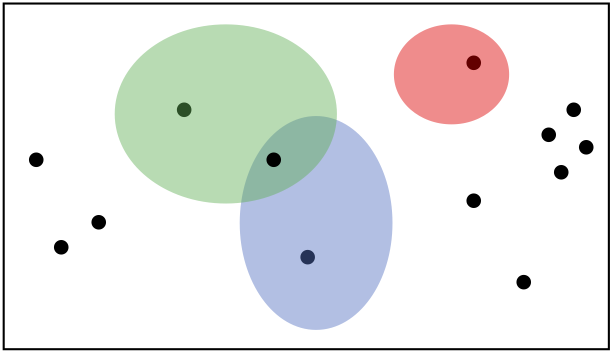
\includegraphics[width=2.5in]{venndiagram-cropped.png}
\caption{The universe of possible attacks against a cryptographic scheme or
protocol.} 
\label{fig:venndiagram}
\end{wrapfigure}


This is not to say that theory, modeling, and formal analysis aren't critical to
applied cryptography. Most obviously we will be building off the deep literature
from theoretical cryptography, and without that theory we would be lost. More
directly, theory provides us powerful tools to help us rule out large
classes of attacks for deployed schemes, that complement and strengthen the one-at-a-time
approach of simple attack-driven investigations. 
One can visualize this process for a particular
scheme as shown in \figref{fig:venndiagram}, which means to depict the universe of all
possible attacks and those attacks covered by different analysis approaches. Each point in
this universe represents an implementable attack against an instantiation 
of the system, which may or may not succeed, and the goal of the analyst is to rule out
the efficacy of as many such attacks as possible.  The black dots
represent one-at-a-time investigation ruling out individual attacks, the
green circle might represent formal reduction-based analyses, the blue circle
symbolic analyses, and the red circle an analysis of some class of side-channel
attacks.  Of course this is highly abstracted, but gives a sense of the
thinking: formal modeling and analysis can help rule out larger classes of
attacks, but certainly will miss things that fall outside the scope of the
model. By combining approaches in a thoughtful manner combined with normative
intuition, one achieves better coverage and can spot attack strategies that may
be more likely to work.

To make this kind of approach work, though, we must have a mastery of modeling
and formal analysis tools. Gaining that mastery is the subject of this course.






\newpage
%%%%%%%%%%%%%%%%%%%%%%%%%%%%%%%%%%%%%%%%%%%%%%%%%%%%%%%%%%%%%%%%%%%%%%%%%%%%%%%%
\section{Preliminaries and Notation}
\label{sec:notation}

We collect here some notation that we will use throughout these notes. 
\tnote{If you introduce new notation in writing up a lecture, please consider
adding it here.} 


\paragraph{Basics.}
We most often denote sets by calligraphic, capital letters, such as $\calX$,
$\calY$, $\calZ$. A discrete probability distribution is a set $\Omega$, the
event space, together with a
function~$p\Colon\Omega\rightarrow[0,1]$ for which $\sum_{\omega\in\Omega}
p_\Omega(\omega) = 1$.
We write $p_\Omega$ when we need to disambiguate the event space, but
otherwise simply $p$ when $\Omega$ is clear from context. We will also,
following convention, often write $\Pr[\omega]$ instead of $p(\omega)$.
The support of $p$ is defined to be the set $\supp(p) = \{\omega \;|\; \omega
\in \Omega \land p(\omega) > 0\}$, 
i.e., the set of all points in $\Omega$ that have non-zero probability.  
As a slight abuse of notation, we can write 
$\Pr[\calS] = p(\calS) = \sum_{\omega\in\calS} p(\omega)$ for any set $\calS \subseteq \Omega$. 

A random variable $X$ is a map $Y\Colon\Omega\rightarrow\calX$ from some event
space $\Omega$ with associated probability distribution $p_\Omega$ over a  set
$\Omega$. So for some other set $\calS$ we let $\Pr[X\in\calS] = \Pr[\{\omega
\;|\; X(\omega) \in \calS\}]$ to be the probability that the random variable
takes on a value in $\calS$, over the probability distribution $p_\Omega$.

We use the language of probability as the foundation for formalizing
cryptographic algorithms, security, and more. Interestingly the probability
spaces involved get complicated quickly, and a common problem is that they end 
ambiguous. We will therefore rely on a crutch that has proved quite useful for
communicating, and reasoning about, probability distributions.


\paragraph{Pseudocode games.} We fix some pseudocode language to describe
security models, cryptographic algorithms, and more. Roughly we will follow the
notational tradition established by Bellare and Rogaway in the
2000s~\cite{bellare2006security}, but using slightly different syntax/symantecs that are
based most closely on a treatment from~\cite{ristenpart2011careful}.  Code-based
games are convenient for more precisely defining probability spaces, which are
what we use to model security and correctness goals, algorithms, and more.  

%We follow~\cite{BR06} 
%with some differences.
We will use procedures, variables, and typical
programming statements (such as operators, loops, procedure calls, etc.).
Typical statements are shown in \figref{fig:statements}.
We do not provide a formal specification of the programming language,
see~\cite[Appendix B]{bellare2006security} for an example of doing so. 
%Games include
%procedures, variables, and typical programming 
%statements (operators, loops, etc.). 
We will rely on some conventions to help make sense of games.
Types should be understable
from context. The names of syntactic objects (procedures, variables, etc.)
must be distinct.  Variables are implicitly 
initialized to default values:  integer variables are set
to 0, arrays are everywhere~$\bot$, etc. Here $\bot$ is a distinguished symbol
by tradition used to denote an error in the cryptographic literature.
By distinguished we mean that it assumed to not be used for any other reason,
not appearing in alphabets over which strings are taken, etc.


\begin{wrapfigure}{r}{3in}
\gamesfontsize
\begin{tabular}{lp{2in}}
\toprule
$x \gets y$ & Assignment\\
$x \getsr \calX$ & Uniform sampling from a set\\
$z \getsr P(x,y)$ & Call a randomized procedure\\
$z \gets P(x,y)$ & Call a deterministic procedure\\
Ret $x$ & Return from a procedure\\
$z \gets x \concat y$ & String concatenation\\
$(x,y) \getparse{n} z$ & Parse string $z$ s.t.~$|x| = n$\\
\bottomrule
\end{tabular}
\caption{Some statements used in our games.}
\label{fig:statements}
\end{wrapfigure}


A \textit{procedure} is a sequence of statements together 
with zero or more variable inputs and zero or more 
outputs. %
%Variables are by default local, meaning they can only be 
%used within a single procedure, but they retain their state 
%between calls to the procedure. %
An \emph{unspecified procedure} is a procedure whose pseudocode, inputs, and
outputs are understood from context.  We will see some examples of
unspecified procedures, the most frequent in our security games being the 
\emph{adversary} which is often left unspecified. 
%
%
A call to a procedure requires providing it with inputs, running its sequence of
statements, and returning its output. We will interchangeably use the term call
and \emph{query} for procedure invocation.
A procedure~$P$ can itself query other
procedures. The set of procedures $Q_1,\ldots,Q_k$ called by a procedure are
statically fixed, and we require that there are no type mismatches in inputs and
outputs. 

Say that the code of~$P$ expects to be able to call~$k$ distinct procedures.
We will write $P^{Q_1,Q_2,\ldots,Q_k}$ to denote that these calls are
handled by $Q_1,Q_2,\ldots,Q_k$ and implicitly assume (for all $i\in[k]$) that there are no
syntactic mismatches between the calls that~$P$ makes to~$Q_i$ and the inputs
of~$Q_i$, as well as between the return values of~$Q_i$
and the return values expected by~$P$.   
%We stress that~$P$ does not
%call~$Q_i$ by name, but rather calls to a procedure that is
%instantiated by~$Q_i$.

We assume that all procedures eventually halt, regardless of randomness used, 
returning their outputs, at which point execution returns to the 
calling procedure.
Two procedures~$P_1$ and~$P_2$ are said to 
\emph{export the same interface} 
if their inputs and outputs have the same number and types. 

Variables will be local by default, meaning they can only be used within a
single procedure. Variables are static, meaning that they retain their 
state between calls to the procedure. It will be convenient to 
allow sharing of variables at times, for which we use a 
\textit{collection of procedures}. This is a set 
of one or more procedures whose variables have scope covering all of the
procedures. We will denote a collection of procedures using 
a common prefix ending with a period, so for example~$(P.x,P.y,\ldots)$,
Sometimes we will use the term interfaces for the specific prefixes of the a
collection of procedures~$P$. 

A \emph{main procedure} is a special procedure that takes no inputs and has some
output.  We will mark it by \main{} (though below
we'll see some syntactic sugar that provides greater brevity).  No procedure may
call~\main{}, it can access all the variables of other specified procedures
(though not unspecified procedures). 

A game consists of a main procedure together with a set of zero or more
specified procedures. We write $\G$ for a game. A game may also make use of
unspecified procedures (such as adversaries), which we enumerate as
superscripts, e.g., $\G^{P_1,P_2,\ldots,P_k}$. In most games used as security
definitions, one (or more) of the unspecified procedures will be called the
adversary, most often denoted by~$\advA$. For a given instantiation of the
unspecified procedures, one can run a game: execute its
statements starting with the designated \main{} procedure, and ultimately
outputing whatever \main{} returns.  

\paragraph{Run times and random variables.} Games can make random choices, due
to the supported statements for sampling according to a distribution. We can
associate to games a model of computation, which specifies how much running each
(type of) statement costs in terms of time, memory, or both.   A typical model
is to assign to each statement the same abstract unit cost, and the run time
then becomes the number of statements executed in the course of the game. 
When procedures are called, we attribute the unit cost of the call statement to
the caller and the remaining cost of executing the procedure's statements to the
callee. 

By default we will require that games terminate in some finite number of
steps~$\runtime$, and clarify explicitly when this does not hold. The number of
queries made by the main procedure, or any other procedure for that matter
including unspecified ones, is
therefore also upper bound by $\runtime$. We  may often limit the number of
queries made by an adversary to some maximum number $\numqueries \le \runtime$. 

Given these finiteness conditions, we similarly know that there is a finite
limit on the number of random samples made in a game. Since we restricted to 
random sampling from finite sets, we have that for any game $\G$ 
there is an event space~$\Omega_\G$ and an associated probability distribution
defining the output of the game $\G$. Given our restrictions, $\Omega_\G$ is a
set of possible values, the cross-product of all the random sampling procedures
within $\G$. We sometimes refer to $\Omega_\G$ as the \emph{coins} of the game.
For some fixed unspecified procedures
$P_1,\ldots,P_k$ we denote the event that executing the game
$\G^{P_1,\ldots,P_k}$ outputs a particular value $y$ by
``$\G^{P_1,\ldots,P_k}\Rightarrow y$'' and the associated probability over
$\Omega_\G$ is denoted $\Pr[\G^{P_1,\ldots,P_k}\Rightarrow y]$. When $y$ is clear
from context we will omit it, writing instead $\Pr[\G^{P_1,\ldots,P_k}]$.  
For example, we will often have games output a boolean and then
$y$ will most often be the value \true.

We can similarly associate to any variable within a game an event within
$\Omega_\G$. These can also be equivalently considered to be random variables on
domain $\Omega_G$. Our convention will be to overload notation, and define the
event that a variable $X$ in a game $\G$ takes on a certain value $y$ as simply
``$X = y$'' with associated probability $\Pr[X = y]$ over the coins of
$\Omega_\G$. 


\paragraph{Runnable games.}  We want to emphasize a point, which is that games
are by our conventions above runnable. That means that, once any unspecified
procedures are fixed, you could write a program in a conventional programming
language, and actually run the game on a real computer. Obviously like with all
abstract algorithms, the actual run times will vary, but assuming relative
efficiency the game will complete.  

It relatively frequently arises in proofs that one deviates from runnable games.
A common example is logic of the following form. Let $\advA$ be an adversary,
and consider a game $\G^\advA$. Remember we implicitly assume that $\advA$ is
compatible with $\G$, and we have that $\G^\advA$ is runnable.  Now consider the
set of all adversaries compatible with $\advA$, and let $\advA_{\max}$ be the
member of this set that maximizes $\Pr[\G^\advA \Rightarrow \true]$. But now
$\G^{\advA_{\max}}$ is no longer runnable, because $\advA_{\max}$ is not
concretely specified. While mathematically $\advA_{\max}$ is well-defined, there
is no clear way to write down its code, even given the code defining~$\advA$.
We will try whenever possible to avoid such arguments, as they have various
subtle implications that are, in general, not great for making 
clear claims about security. 






%\newpage
%%%%%%%%%%%%%%%%%%%%%%%%%%%%%%%%%%%%%%%%%%%%%%%%%%%%%%%%%%%%%%%%%%%%%%%%%%%%%%%%%
\section{Ciphers and Initial Security Notions}
\label{sec:se}

\paragraph{Ciphers.}
We start by defining a cipher. A cipher $\cipher = (\cipherE,\cipherD)$ is
defined by a a pair of deterministic algorithms $\cipherE$ and $\cipherD$.  To
any cipher $\cipher$ we associate sets called the key space $\keyspace$, message
space $\msgspace$, and ciphertext space $\ctxtspace$. We do not surface in the
notation for a cipher these sets, and will require that the association be clear
from context.

The algorithms are two-input. Enciphering takes a key $K \in \keyspace$ and
message $M \in \msgspace$, and outputs a ciphertext $C \in \ctxtspace$. Because
$\cipherE$ is deterministic, we can equally formalize it as a map 
$\cipherE\Colon\keyspace\times\msgspace\rightarrow\ctxtspace$. For a given key
$K$ we let $\cipherE_K\Colon\msgspace\rightarrow\ctxtspace$ be defined by
$\cipherE_K(M) = \cipherE(K,M)$ for all $M \in \msgspace$.  Deciphering takes a key $K\in \keyspace$ and ciphertext
$C \in \ctxtspace$ and outputs a message $M \in \msgspace$. Again, we can view
it as a map $\cipherD\Colon\keyspace\times\ctxtspace\rightarrow\msgspace$. 

Both $\cipherE$ and $\cipherD$ must be efficiently computable for all $K \in
\keyspace$.  (We have not defined efficiently computable, and use the term here
informally.) We require that a cipher be correct, meaning that for
$\cipherD_K(\cipherE_K(M)) = M$ for all $M$. 

\paragraph{Security notions.} What do we intuitively expect of a cipher?
Minimally:
\begin{itemize}
\item Secret key should remain secret
\item Message should remain secret
\end{itemize}
Let's try to formalize these notions.
\begin{itemize}
\item TKR security
\item KR security
\item (ot-)IND security
\end{itemize}


\begin{figure}[p]
\fpage{.45}{
\underline{$\TKR^\advA_\cipher$}\\[1pt]
$K \getsr \keyspace$\\
$K^* \getsr \advA^\Fn$\\
Ret $(K = K^*)$\medskip

\underline{$\Fn(M)$}\\
$C \gets \cipherE_K(M)$\\
Ret $C$
}
\end{figure}

We let $\TKR_\cipher$-advantage of a $\TKR_\cipher$-adversary $\advA$ be defined by 
\bnm
  \AdvTKR{\cipher}{\advA} = \Prob{\TKR^\advA_\cipherE \Rightarrow\true}  \;.
\enm

\begin{figure}[p]
\fpage{.45}{
\underline{$\KR^\advA_\cipher$}\\[1pt]
$K \getsr \keyspace$\\
$K^* \getsr \advA^\Fn$\\
$\win \gets \true$\\ 
For $M \in \calX$:\\
\ind If $\cipherE_{K^*}(M) \ne \cipherE_{K}(M)$ then\\
\ind\ind $\win \gets \false$\\
Ret $\win$\medskip

\underline{$\Fn(M)$}\\
$\calX \gets \calX \cup \{M\}$\\
$C \gets \cipherE_K(M)$\\
Ret $C$
}
\end{figure}

We let $\KR_\cipher$-advantage of a $\KR_\cipher$-adversary $\advA$ be defined by 
\bnm
  \AdvKR{\cipher}{\advA} = \Prob{\KR^\advA_\cipherE \Rightarrow\true}  \;.
\enm


\begin{figure}[p]
\fpage{.45}{
\underline{$\OTIND^\advA_\cipher$}\\[1pt]
$K \getsr \keyspace$\\
$b \getsr \bits$\\
$b' \getsr \advA^\Fn$\\
Ret $(b = b')$\medskip

\underline{$\Fn(M_0,M_1)$}\\
$C \gets \cipherE_K(M_b)$\\
Ret $C$
}
\end{figure}

We let $\OTIND_\cipher$-advantage of a $\OTIND_\cipher$-adversary $\advA$ be defined by 
\bnm
  \AdvOTIND{\cipher}{\advA} = 2\cdotsm\Prob{\OTIND^\advA_\cipherE \Rightarrow\true} - 1  \;.
\enm

\bigskip
\bigskip


\begin{itemize}
\item First example: Our simple OTP cipher is not $\TKR$ secure? Go over example: $\advA$
queries once on arbitrary message, recovers $K$ by computing $M \oplus C$. This
is guaranteed to succeed because $M \oplus C$ uniquely defines $K$. What does
this mean? Isn't OTP considered secure? Shannon said so!
%
\item Second example: Give toy cipher $\cipher$ for which $\TKR_\cipher$ has
$\AdvTKR{\cipher}{\advA} = 0$ for any adversary $\advA$. What is it?
$\cipherE(K,M) = M$. It is correct 
%
\item Third example: Exhaustive key search attack against generic
cipher. Emphasize that lower-bounding the efficacy of this is not possible in
general. Why? Consider toy identity cipher! 
%
\item Discuss the KR definition. Rules out the
identity map as being relevant. Lower-bounding security is 
%
\item Shannon's perfect secrecy (one-time left-or-right indistinguishability). 
\end{itemize}

\begin{theorem}
Let $\cipher$ be a cipher. For any $\TKR_\cipher$-adversary $\advA$, we give a
$\KR_\cipher$-adversary $\advB$ such that 
  $\AdvKR{\cipher}{\advA} = \AdvTKR{\cipher}{\advB}$.
\end{theorem}

In our theorem statements including reductions,  we need to interpret the words
``we give a''. We will focus on concrete, specified reductions. That means that
the adversary $\advB$ not only exists, but is fully specified  --- minus the
details of $\advA$ ---  within the proof.  In particular, if you give someone
$\advA$ then $\advB$ becomes runnable.  Runnable reductions are generally
speaking easier to interpret when it comes to implied security guarantees. They
even allow us to use the human-ignorance model~\cite{rogaway2006formalizing}
which, roughly, states that a reduction even to a mathematically easy assumption
can still be meaningful. (We will revisit this particular issue with an example
in the context of collision resistance.)
An example of a non-runnable $\advB$ would be one that includes some constant
value that we know exists, but don't know an exact value for. This comes up in
various arguments, and can cause problems in interpreting the reduction in terms
of concrete security.  This issue is subtle and we will revisit it.

The takeaway here being that one interprets ``we give a'' to mean runnable
adversaries that are specified fully in the proof. (Or when brevity is at stake,
specified to a leave of detail that the average reader could specify it in
detail easily.)  When we deviate from this convention we should remark on it.




\begin{theorem}
Let $\cipher$ be the OTP cipher. Then for any single-query
$\OTIND_\cipher$-adversary $\advA$ it holds that $\AdvOTIND{\cipher}{\advA} = 0$. \end{theorem}


\begin{theorem}
Let $\cipher$ be a cipher defined 
over $(\keyspace,\msgspace,\ctxtspace)$ such that for any $\OTIND_\cipherE$-adversary 
$\advA$ it holds that $\AdvOTIND{\cipher}{\advA} = 0$. Then $|\keyspace| \ge
|\msgspace|$. 
\end{theorem}


\begin{figure}
\fpage{.45}{
\underline{$\advA_{\textrm{eks}}$}\\[1pt]
$C \gets \Fn(M)$\\
For $K \in \calK$ do:\\
\ind If $C = \cipherE(K,M)$ then\\
\ind\ind Return $K$\\
Return $\bot$
}
\end{figure}

\paragraph{PRPs and PRFs.}

\begin{itemize}
\item Basic cipher definitions, key recovery attacks
\item PRP and PRF definitions
\item PRP/PRF switching lemma
\begin{itemize}
  \item Incorrect conditioning argument 
  \item Correct game-playing argument
\end{itemize}
\item PRP from PRF constructions: Feistel networks
\item Luby-Rackoff proof
\end{itemize}


\begin{figure}
\fpage{.15}{
\underline{$\PRP_{\cipher}^\advA$}\\
$b \getsr \bits$\\
$K \getsr \keyspace$\\
$\pi \getsr \Perm(n)$\\
$b' \getsr \advA^\Fn$\\
Return $(b = b')$\medskip

\underline{$\Fn(M)$}\\
If $b = 1$ then\\
\ind Return $\cipherE_K(M)$\\
Return $\pi(M)$
}
\end{figure}

\bnm
\AdvPRP{\cipher}{\advA} = 2\cdotsm\Prob{\PRP^\advA_\cipher\Rightarrow\true}- 1
\enm

\begin{figure}
\hfpages{.25}{
\underline{$\PRP1_{\cipher}^\advA$}\\
$K \getsr \keyspace$\\
$b' \getsr \advA^\Fn$\\
Return $b'$\medskip

\underline{$\Fn(M)$}\\
Return $\cipherE_K(M)$\\
}{
\underline{$\PRP0_{\cipher}^\advA$}\\
$\pi \getsr \Perm(n)$\\
$b' \getsr \advA^\Fn$\\
Return $b'$\medskip

\underline{$\Fn(M)$}\\
Return $\pi(M)$\\
}


\end{figure}


\begin{figure}
\hfpages{.25}{
\underline{$\PRF1_{\cipher}^\advA$}\\
$K \getsr \keyspace$\\
$b' \getsr \advA^\Fn$\\
Return $b'$\medskip

\underline{$\Fn(M)$}\\
Return $\cipherE_K(M)$\\
}{
\underline{$\PRF0_{\cipher}^\advA$}\\
$\rho \getsr \Func(n,n)$\\
$b' \getsr \advA^\Fn$\\
Return $b'$\medskip

\underline{$\Fn(M)$}\\
Return $\rho(M)$\\
}


\end{figure}



\begin{lemma} Let $\cipher$ be a cipher with ciphertext space $\bits^n$. 
Let $\advA$ be an adversary making at most $q$ queries. Then
\bnm
  \left| \Prob{\PRF0_\cipher^\advA\Rightarrow 1} 
      - \Prob{\PRP0_\cipher^\advA\Rightarrow1} \right| \le \frac{q^2}{2^n}  \;.
\enm
\end{lemma}

\begin{align*}
&\left| \Prob{\PRP0_\cipher^\advA\Rightarrow 1} 
      - \Prob{\PRF0_\cipher^\advA\Rightarrow1} \right| \\ 
     &\myInd\myInd\myInd =  \left|\Prob{\G0} - \Prob{\PRF0_\cipher^\advA\Rightarrow1} \right|  \\
     &\myInd\myInd\myInd  =  \left|\Prob{\G1} - \Prob{\PRF0_\cipher^\advA\Rightarrow1} \right|  \\
     &\myInd\myInd\myInd  \le \left|\Prob{\G2} + \Prob{\bad_2} - \Prob{\PRF0_\cipher^\advA\Rightarrow1} \right|\\
     &\myInd\myInd\myInd  = \Prob{\bad_2}\\
     &\myInd\myInd\myInd  \le \frac{q^2}{2^n}\\
\end{align*}

\begin{lemma} Let $\G$, $\Hgame$ be games that are identical-until-bad and $y$ be any
value. Then
\bnm
  \big| \Prob{\G\Rightarrow y} 
      - \Prob{\Hgame\Rightarrow y} \big| \le \Prob{\Hgame\setsbad} = \Prob{\G\setsbad}  \;.
\enm
\end{lemma}


\begin{figure}
\hfpagess{.20}{.20}{
\underline{$\G0$}\\[2pt]
$b' \getsr \advA^\Fn$\\
Return $b'$\medskip

\underline{$\Fn(M)$}\\
If $\TabF[M] = \bot$ then\\
\ind $\TabF[M] \getsr \bits^n \setminus \TabF$\\
Return $\TabF[M]$
}{
\underline{\fbox{$\G1$} \;\;\; $\G2$}\\[2pt]
$b' \getsr \advA^\Fn$\\
Return $b'$\medskip

\underline{$\Fn(M)$}\\
$C \getsr \bits^n$\\
If $C \in \TabF$ then\\
\ind $\badtrue$\\
\ind \fbox{$C \getsr \bits^n \setminus \TabF$}\\
$\TabF[M] \gets C$\\
Return $\TabF[M]$
}


\end{figure}



\begin{figure}
\hfpagessss{.20}{.20}{.20}{.20}{
\underline{$\G0$}\\[2pt]
$K \getsr \bits^k$\\
$b' \getsr \advA^\Fn$\\
Return $b'$\medskip

\underline{$\Fn(LR)$}\\
$L_1 \gets R$\\
$R_1 \gets L \oplus F_K(\langle 1\rangle \concat R)$\\
$L_2 \gets R_1$\\
$R_2 \gets L_1 \oplus F_K(\langle 2 \rangle \concat R_1)$\\
$L_3 \gets R_2$\\
$R_3 \gets L_2 \oplus F_K(\langle 3 \rangle \concat R_2)$\\
Return $L_3 \concat R_3$
}{
\underline{$\G1$}\\[2pt]
$\rho \getsr \Func(2n,n)$\\
$b' \getsr \advA^\Fn$\\
Return $b'$\medskip

\underline{$\Fn(LR)$}\\
$L_1 \gets R$\\
$R_1 \gets L \oplus \rho(\langle 1\rangle \concat R)$\\
$L_2 \gets R_1$\\
$R_2 \gets L_1 \oplus \rho(\langle 2 \rangle \concat R_1)$\\
$L_3 \gets R_2$\\
$R_3 \gets L_2 \oplus \rho(\langle 3 \rangle \concat R_2)$\\
Return $L_3 \concat R_3$
}{
\underline{$\fbox{\G2}$\;\;\;\G3}\\[2pt]
$b' \getsr \advA^\Fn$\\
Return $b'$\medskip

\underline{$\Fn(LR)$}\\
$L_1 \gets R$\\
If $\TabF[1,R] = \bot$ then\\
\ind $\TabF[1,R] \getsr \bits^n$\\
$R_1 \gets L \oplus \TabF[1,R]$\\
$L_2 \gets R_1$\\
$X_2 \getsr \bits^n$\\
If $\TabF[2,R_1] \ne \bot$ then\\
\ind $\badtrue$\\
\ind \fbox{$X_2 \gets \TabF[2,R_1]$}\\
$\TabF[2,R_1] \gets X_2$\\
$R_2 \gets L_1 \oplus X_2$\\
$L_3 \gets R_2$\\
$X_3 \getsr \bits^n$\\
If $\TabF[3,R_2] \ne \bot$ then\\
\ind $\badtrue$\\
\ind \fbox{$X_3 \gets \TabF[2,R_2]$}\\
$\TabF[3,R_2] \gets X_3$\\
$R_3 \gets L_2 \oplus X_3$\\
Return $L_3 \concat R_3$
}{
\underline{$\G4$}\\[2pt]
$b' \getsr \advA^\Fn$\\
Return $b'$\medskip

\underline{$\Fn(LR)$}\\
$L_1 \gets R$\\
If $\TabF[1,R] = \bot$ then\\
\ind $\TabF[1,R] \getsr \bits^n$\\
$R_1 \gets L \oplus \TabF[1,R]$\\
$L_2 \gets R_1$\\
If $\TabF[2,R_1] \ne \bot$ then\\
\ind $\badtrue$\\
$\TabF[2,R_1] \gets 1$\\
$R_2 \getsr \bits^n$\\
$L_3 \gets R_2$\\
%$X_3 \getsr \bits^n$\\
If $\TabF[3,R_2] \ne \bot$ then\\
\ind $\badtrue$\\
$\TabF[3,R_2] \gets 1$\\
$R_3 \getsr \bits^n$\\
Return $L_3 \concat R_3$
}
\end{figure}

\begin{figure}
\fpage{.25}{
\underline{$\advB^\Fn$}\\[2pt]
$K \getsr \bits^k$\\
$b' \getsr \advA^\FnSim$\\
Return $b'$\medskip

\underline{$\FnSim(LR)$}\\
$L_1 \gets R$\\
$R_1 \gets L \oplus \Fn(\langle 1\rangle \concat R)$\\
$L_2 \gets R_1$\\
$R_2 \gets L_1 \oplus \Fn(\langle 2 \rangle \concat R_1)$\\
$L_3 \gets R_2$\\
$R_3 \gets L_2 \oplus \Fn(\langle 3 \rangle \concat R_2)$\\
Return $L_3 \concat R_3$
}
\end{figure}

\newpage

\begin{theorem}
Let $\Feistel$ be the 3-round Feistel cipher using round function 
$F\Colon\bits^k\times\bits^n\rightarrow \bits^n$. For any
$\PRP_\cipher$-adversary $\advA$ making at most $q$ queries 
we give an $\PRF_F$-adversary $\advB$ making at most $3q$ queries such that
\bnm
  \AdvPRP{\Feistel}{\advA} \le \AdvPRF{F}{\advB} + \frac{2q^2}{2^n} +
  \frac{q^2}{2^{2n}} \;.
\enm
\end{theorem}



\begin{align*}
\AdvPRP{\cipher}{\advA} 
    &= \left|\Prob{\PRP1^\advA_\cipher} - \Prob{\PRP0^\advA_\cipher}\right|\\
    &= \left|\Prob{\G0} - \Prob{\PRP0^\advA_\cipher}\right|\\
    &\le \left|\Prob{\G1} + \AdvPRF{F}{\advB} - \Prob{\PRP0^\advA_\cipher}\right|\\
    &=   \left|\Prob{\G2} + \AdvPRF{F}{\advB} - \Prob{\PRP0^\advA_\cipher}\right|\\
    &\le \left|\Prob{\G3} + \Prob{\bad_3} + \AdvPRF{F}{\advB} - \Prob{\PRP0^\advA_\cipher}\right|\\
    &= \left|\Prob{\G4} + \Prob{\bad_4} + \AdvPRF{F}{\advB} - \Prob{\PRP0^\advA_\cipher}\right|\\
    &\le \left|\Prob{\PRP0^\advA_\cipher} + \frac{q^2}{2^{2n}} + \Prob{\bad_4} + \AdvPRF{F}{\advB} - \Prob{\PRP0^\advA_\cipher}\right|\\
    &= \frac{q^2}{2^{2n}} + \Prob{\bad_4} + \AdvPRF{F}{\advB}\\
    &\le \frac{q^2}{2^{2n}} + \frac{2q^2}{2^n} + \AdvPRF{F}{\advB}\\
\end{align*}


\newpage
%%%%%%%%%%%%%%%%%%%%%%%%%%%%%%%%%%%%%%%%%%%%%%%%%%%%%%%%%%%%%%%%%%%%%%%%%%%%%%%%
\section{Ciphers and Initial Security Notions}
\label{sec:se}

\paragraph{Ciphers.}
We start by defining a cipher. A cipher $\cipher = (\cipherE,\cipherD)$ is
defined by a a pair of deterministic algorithms $\cipherE$ and $\cipherD$.  To
any cipher $\cipher$ we associate sets called the key space $\keyspace$, message
space $\msgspace$, and ciphertext space $\ctxtspace$. We do not surface these sets in the
notation for a cipher, and we will require that the association be clear
from context.

Each algorithm has two inputs. Enciphering takes a key $K \in \keyspace$ and
message $M \in \msgspace$, and outputs a ciphertext $C \in \ctxtspace$. Because
$\cipherE$ is deterministic, we can equally formalize it as a map 
$\cipherE\Colon\keyspace\times\msgspace\rightarrow\ctxtspace$. For a given key
$K$ we let $\cipherE_K\Colon\msgspace\rightarrow\ctxtspace$ be defined by
$\cipherE_K(M) = \cipherE(K,M)$ for all $M \in \msgspace$.  Deciphering takes a key $K\in \keyspace$ and ciphertext
$C \in \ctxtspace$ and outputs a message $M \in \msgspace$. Again, we can view
it as a map $\cipherD\Colon\keyspace\times\ctxtspace\rightarrow\msgspace$. 

Both $\cipherE$ and $\cipherD$ must be efficiently computable for all $K \in
\keyspace$.  (We have not defined efficiently computable and use the term here
informally.) We require that a cipher be correct, meaning that
$\forall M \in \msgspace, \forall K \in \keyspace, \cipherD_K(\cipherE_K(M)) = M$.

\paragraph{Example.} One simple example of a cipher is the \textbf{one-time pad} (OTP). Let $\keyspace = \msgspace=\ctxtspace=\{0,1\}^n$ for some $n \in \N$. Then we define OTP as follows:
\begin{align*}
&\cipherE_K(M) = M \oplus K \\
&\cipherD_K(C) = C \oplus K
\end{align*}
Claude Shannon proved that OTP is perfectly secure in 1949 \cite{shannon1949communication}.

\paragraph{Security notions.} What do we intuitively expect of a cipher?
Minimally:
\begin{itemize}
\item The secret key should remain secret.
\item The message should remain secret.
\end{itemize}

Let's try to formalize these notions. We will start with a security notion called \textbf{target key recovery security} (TKR).
As the name suggests, the goal of the adversary is to recover the challenge key given a chosen plaintext attack, meaning the adversary can choose which messages to query to the $\Fn$ oracle. The game pseudocode is provided in \figref{fig:tkr}. We let $\TKR_\cipher$-advantage of a $\TKR_\cipher$-adversary $\advA$ be defined by 
\bnm
\AdvTKR{\cipher}{\advA} = \Prob{\TKR^\advA_\cipherE \Rightarrow\true}  \;.
\enm

\begin{figure}[p]
	\centering
	\fpage{.45}{
		\underline{$\TKR^\advA_\cipher$}\\[1pt]
		$K \getsr \keyspace$\\
		$K^* \getsr \advA^\Fn$\\
		Ret $(K = K^*)$\medskip
		
		\underline{$\Fn(M)$}\\
		$C \gets \cipherE_K(M)$\\
		Ret $C$
	}
	\caption{The target key recovery game.}
	\label{fig:tkr}
\end{figure}


We must now ask ourselves how well TKR captures the security of a cipher. Let us first try to analyze the security of OTP using this definition. Notice that OTP actually fails to provide TKR security, which we show with the following adversary.
\begin{align*}
&\underline{\textbf{adversary } \advA} \\
&K \gets \Fn(0^n) \\
&\text{Return } K 
\end{align*}	

$\advA$ simply queries for $0^n$, which returns $0^n \oplus K = K$, thereby recovering the challenge key with $\AdvTKR{\cipher}{\advA} = 1$. This then means that OTP is actually insecure according to the TKR security definition. But as we noted earlier, OTP is considered secure! Our definition then fails to capture the security of OTP. 

Now consider the identity cipher $\cipherE_{K}(M) = M$ for $\keyspace=\{0,1\}^k$. Since the cipher simply returns the message, no information about the key is included in the ciphertext. The best an adversary can do is return a random key, which has probability $2^{-k}$ of being the correct target key.
Then for any adversary $\advA$, it holds that $\AdvTKR{\cipher}{\advA} = 2^{-k}$, meaning the identity cipher is secure! Clearly this is not the case, and thus TKR security does not provide message confidentiality. Furthermore, this security notion is ``unfair'' to an adversary, since there can be many keys that are \textit{consistent} on a query transcript. 

\begin{figure}[p]
	\centering
	\fpage{.45}{
		\underline{$\KR^\advA_\cipher$}\\[1pt]
		$\win \gets \false$\\
		$K \getsr \keyspace$\\
		$K^* \getsr \advA^\Fn$\\ 
		For $M \in \calX$:\\
		\ind If $\cipherE_{K^*}(M) \ne \cipherE_{K}(M)$ then\\
		\ind\ind $\win \gets \false$\\
		Return $\win$\medskip
		
		\underline{$\Fn(M)$}\\
		$\win \gets \true$ \\
		$\calX \gets \calX \cup \{M\}$\\
		$C \gets \cipherE_K(M)$\\
		Ret $C$
	}
	\caption{The key recovery game.}
	\label{fig:kr}
\end{figure}

We then look at a different notion called \textbf{key recovery security} (KR). Under this definition, if an adversary outputs a key that is consistent with the query transcript, then it wins. The game pseudocode is provided in \figref{fig:kr}. We let $\KR_\cipher$-advantage of a $\KR_\cipher$-adversary $\advA$ be defined by 
\bnm
\AdvKR{\cipher}{\advA} = \Prob{\KR^\advA_\cipherE \Rightarrow\true}  \;.
\enm

\paragraph{Comparing security definitions.} We can formally compare security definitions. To show that some definition DEF1 does not imply another definition DEF2, we can show a \textit{counter-example}. This requires producing a scheme such that we can show that no (reasonable) DEF1-adversary has a good advantage. We then give a DEF2-adversary that gets good DEF2 advantage.

Conversely, to show that DEF1 does imply DEF2, we can show a \textit{reduction}. This requires converting a DEF2-adversary $\advA$ into a DEF1-adversary $\advB$ such that $\advB$'s DEF1 advantage upper bounds $\advA$'s DEF2 advantage. 


\begin{table}
	\centering
	\begin{tabular}{c | c}
		DEF1 $\not \Rightarrow$ DEF2 & We show a counter-example. \\ \hline
		DEF1 $\Rightarrow$ DEF2 & We show a reduction.
	\end{tabular}
\end{table}

\begin{itemize}
	\item First example: Our simple OTP cipher is not $\TKR$ secure? Go over example: $\advA$
	queries once on arbitrary message, recovers $K$ by computing $M \oplus C$. This
	is guaranteed to succeed because $M \oplus C$ uniquely defines $K$. What does
	this mean? Isn't OTP considered secure? Shannon said so!
	%
	\item Second example: Give toy cipher $\cipher$ for which $\TKR_\cipher$ has
	$\AdvTKR{\cipher}{\advA} = 0$ for any adversary $\advA$. What is it?
	$\cipherE(K,M) = M$. It is correct 
	%
	\item Third example: Exhaustive key search attack against generic
	cipher. Emphasize that lower-bounding the efficacy of this is not possible in
	general. Why? Consider toy identity cipher! 
	%
	\item Discuss the KR definition. Rules out the
	identity map as being relevant. Lower-bounding security is 
	%
	\item Shannon's perfect secrecy (one-time left-or-right indistinguishability). 
\end{itemize}


\begin{itemize}
	\item KR security
	\item (ot-)IND security
\end{itemize}


\begin{figure}[p]
\fpage{.45}{
\underline{$\OTIND^\advA_\cipher$}\\[1pt]
$K \getsr \keyspace$\\
$b \getsr \bits$\\
$b' \getsr \advA^\Fn$\\
Ret $(b = b')$\medskip

\underline{$\Fn(M_0,M_1)$}\\
$C \gets \cipherE_K(M_b)$\\
Ret $C$
}
\end{figure}

We let $\OTIND_\cipher$-advantage of a $\OTIND_\cipher$-adversary $\advA$ be defined by 
\bnm
  \AdvOTIND{\cipher}{\advA} = 2\cdotsm\Prob{\OTIND^\advA_\cipherE \Rightarrow\true} - 1  \;.
\enm

\bigskip
\bigskip




\begin{theorem}
Let $\cipher$ be a cipher. For any $\TKR_\cipher$-adversary $\advA$, we give a
$\KR_\cipher$-adversary $\advB$ such that 
  $\AdvKR{\cipher}{\advA} = \AdvTKR{\cipher}{\advB}$.
\end{theorem}

In our theorem statements including reductions,  we need to interpret the words
``we give a''. We will focus on concrete, specified reductions. That means that
the adversary $\advB$ not only exists, but is fully specified  --- minus the
details of $\advA$ ---  within the proof.  In particular, if you give someone
$\advA$ then $\advB$ becomes runnable.  Runnable reductions are generally
speaking easier to interpret when it comes to implied security guarantees. They
even allow us to use the human-ignorance model~\cite{rogaway2006formalizing}
which, roughly, states that a reduction even to a mathematically easy assumption
can still be meaningful. (We will revisit this particular issue with an example
in the context of collision resistance.)
An example of a non-runnable $\advB$ would be one that includes some constant
value that we know exists, but don't know an exact value for. This comes up in
various arguments, and can cause problems in interpreting the reduction in terms
of concrete security.  This issue is subtle and we will revisit it.

The takeaway here being that one interprets ``we give a'' to mean runnable
adversaries that are specified fully in the proof. (Or when brevity is at stake,
specified to a leave of detail that the average reader could specify it in
detail easily.)  When we deviate from this convention we should remark on it.




\begin{theorem}
Let $\cipher$ be the OTP cipher. Then for any single-query
$\OTIND_\cipher$-adversary $\advA$ it holds that $\AdvOTIND{\cipher}{\advA} = 0$. \end{theorem}


\begin{theorem}
Let $\cipher$ be a cipher defined 
over $(\keyspace,\msgspace,\ctxtspace)$ such that for any $\OTIND_\cipherE$-adversary 
$\advA$ it holds that $\AdvOTIND{\cipher}{\advA} = 0$. Then $|\keyspace| \ge
|\msgspace|$. 
\end{theorem}


\begin{figure}
\fpage{.45}{
\underline{$\advA_{\textrm{eks}}$}\\[1pt]
$C \gets \Fn(M)$\\
For $K \in \calK$ do:\\
\ind If $C = \cipherE(K,M)$ then\\
\ind\ind Return $K$\\
Return $\bot$
}
\end{figure}

\paragraph{PRPs and PRFs.}

\begin{itemize}
\item Basic cipher definitions, key recovery attacks
\item PRP and PRF definitions
\item PRP/PRF switching lemma
\begin{itemize}
  \item Incorrect conditioning argument 
  \item Correct game-playing argument
\end{itemize}
\item PRP from PRF constructions: Feistel networks
\item Luby-Rackoff proof
\end{itemize}


\begin{figure}
\fpage{.15}{
\underline{$\PRP_{\cipher}^\advA$}\\
$b \getsr \bits$\\
$K \getsr \keyspace$\\
$\pi \getsr \Perm(n)$\\
$b' \getsr \advA^\Fn$\\
Return $(b = b')$\medskip

\underline{$\Fn(M)$}\\
If $b = 1$ then\\
\ind Return $\cipherE_K(M)$\\
Return $\pi(M)$
}
\end{figure}

\bnm
\AdvPRP{\cipher}{\advA} = 2\cdotsm\Prob{\PRP^\advA_\cipher\Rightarrow\true}- 1
\enm

\begin{figure}
\hfpages{.25}{
\underline{$\PRP1_{\cipher}^\advA$}\\
$K \getsr \keyspace$\\
$b' \getsr \advA^\Fn$\\
Return $b'$\medskip

\underline{$\Fn(M)$}\\
Return $\cipherE_K(M)$\\
}{
\underline{$\PRP0_{\cipher}^\advA$}\\
$\pi \getsr \Perm(n)$\\
$b' \getsr \advA^\Fn$\\
Return $b'$\medskip

\underline{$\Fn(M)$}\\
Return $\pi(M)$\\
}


\end{figure}


\begin{figure}
\hfpages{.25}{
\underline{$\PRF1_{\cipher}^\advA$}\\
$K \getsr \keyspace$\\
$b' \getsr \advA^\Fn$\\
Return $b'$\medskip

\underline{$\Fn(M)$}\\
Return $\cipherE_K(M)$\\
}{
\underline{$\PRF0_{\cipher}^\advA$}\\
$\rho \getsr \Func(n,n)$\\
$b' \getsr \advA^\Fn$\\
Return $b'$\medskip

\underline{$\Fn(M)$}\\
Return $\rho(M)$\\
}


\end{figure}



\begin{lemma} Let $\cipher$ be a cipher with ciphertext space $\bits^n$. 
Let $\advA$ be an adversary making at most $q$ queries. Then
\bnm
  \left| \Prob{\PRF0_\cipher^\advA\Rightarrow 1} 
      - \Prob{\PRP0_\cipher^\advA\Rightarrow1} \right| \le \frac{q^2}{2^n}  \;.
\enm
\end{lemma}

\begin{align*}
&\left| \Prob{\PRP0_\cipher^\advA\Rightarrow 1} 
      - \Prob{\PRF0_\cipher^\advA\Rightarrow1} \right| \\ 
     &\myInd\myInd\myInd =  \left|\Prob{\G0} - \Prob{\PRF0_\cipher^\advA\Rightarrow1} \right|  \\
     &\myInd\myInd\myInd  =  \left|\Prob{\G1} - \Prob{\PRF0_\cipher^\advA\Rightarrow1} \right|  \\
     &\myInd\myInd\myInd  \le \left|\Prob{\G2} + \Prob{\bad_2} - \Prob{\PRF0_\cipher^\advA\Rightarrow1} \right|\\
     &\myInd\myInd\myInd  = \Prob{\bad_2}\\
     &\myInd\myInd\myInd  \le \frac{q^2}{2^n}\\
\end{align*}

\begin{lemma} Let $\G$, $\Hgame$ be games that are identical-until-bad and $y$ be any
value. Then
\bnm
  \big| \Prob{\G\Rightarrow y} 
      - \Prob{\Hgame\Rightarrow y} \big| \le \Prob{\Hgame\setsbad} = \Prob{\G\setsbad}  \;.
\enm
\end{lemma}


\begin{figure}
\hfpagess{.20}{.20}{
\underline{$\G0$}\\[2pt]
$b' \getsr \advA^\Fn$\\
Return $b'$\medskip

\underline{$\Fn(M)$}\\
If $\TabF[M] = \bot$ then\\
\ind $\TabF[M] \getsr \bits^n \setminus \TabF$\\
Return $\TabF[M]$
}{
\underline{\fbox{$\G1$} \;\;\; $\G2$}\\[2pt]
$b' \getsr \advA^\Fn$\\
Return $b'$\medskip

\underline{$\Fn(M)$}\\
$C \getsr \bits^n$\\
If $C \in \TabF$ then\\
\ind $\badtrue$\\
\ind \fbox{$C \getsr \bits^n \setminus \TabF$}\\
$\TabF[M] \gets C$\\
Return $\TabF[M]$
}


\end{figure}



\begin{figure}
\hfpagessss{.20}{.20}{.20}{.20}{
\underline{$\G0$}\\[2pt]
$K \getsr \bits^k$\\
$b' \getsr \advA^\Fn$\\
Return $b'$\medskip

\underline{$\Fn(LR)$}\\
$L_1 \gets R$\\
$R_1 \gets L \oplus F_K(\langle 1\rangle \concat R)$\\
$L_2 \gets R_1$\\
$R_2 \gets L_1 \oplus F_K(\langle 2 \rangle \concat R_1)$\\
$L_3 \gets R_2$\\
$R_3 \gets L_2 \oplus F_K(\langle 3 \rangle \concat R_2)$\\
Return $L_3 \concat R_3$
}{
\underline{$\G1$}\\[2pt]
$\rho \getsr \Func(2n,n)$\\
$b' \getsr \advA^\Fn$\\
Return $b'$\medskip

\underline{$\Fn(LR)$}\\
$L_1 \gets R$\\
$R_1 \gets L \oplus \rho(\langle 1\rangle \concat R)$\\
$L_2 \gets R_1$\\
$R_2 \gets L_1 \oplus \rho(\langle 2 \rangle \concat R_1)$\\
$L_3 \gets R_2$\\
$R_3 \gets L_2 \oplus \rho(\langle 3 \rangle \concat R_2)$\\
Return $L_3 \concat R_3$
}{
\underline{$\fbox{\G2}$\;\;\;\G3}\\[2pt]
$b' \getsr \advA^\Fn$\\
Return $b'$\medskip

\underline{$\Fn(LR)$}\\
$L_1 \gets R$\\
If $\TabF[1,R] = \bot$ then\\
\ind $\TabF[1,R] \getsr \bits^n$\\
$R_1 \gets L \oplus \TabF[1,R]$\\
$L_2 \gets R_1$\\
$X_2 \getsr \bits^n$\\
If $\TabF[2,R_1] \ne \bot$ then\\
\ind $\badtrue$\\
\ind \fbox{$X_2 \gets \TabF[2,R_1]$}\\
$\TabF[2,R_1] \gets X_2$\\
$R_2 \gets L_1 \oplus X_2$\\
$L_3 \gets R_2$\\
$X_3 \getsr \bits^n$\\
If $\TabF[3,R_2] \ne \bot$ then\\
\ind $\badtrue$\\
\ind \fbox{$X_3 \gets \TabF[2,R_2]$}\\
$\TabF[3,R_2] \gets X_3$\\
$R_3 \gets L_2 \oplus X_3$\\
Return $L_3 \concat R_3$
}{
\underline{$\G4$}\\[2pt]
$b' \getsr \advA^\Fn$\\
Return $b'$\medskip

\underline{$\Fn(LR)$}\\
$L_1 \gets R$\\
If $\TabF[1,R] = \bot$ then\\
\ind $\TabF[1,R] \getsr \bits^n$\\
$R_1 \gets L \oplus \TabF[1,R]$\\
$L_2 \gets R_1$\\
If $\TabF[2,R_1] \ne \bot$ then\\
\ind $\badtrue$\\
$\TabF[2,R_1] \gets 1$\\
$R_2 \getsr \bits^n$\\
$L_3 \gets R_2$\\
%$X_3 \getsr \bits^n$\\
If $\TabF[3,R_2] \ne \bot$ then\\
\ind $\badtrue$\\
$\TabF[3,R_2] \gets 1$\\
$R_3 \getsr \bits^n$\\
Return $L_3 \concat R_3$
}
\end{figure}

\begin{figure}
\fpage{.25}{
\underline{$\advB^\Fn$}\\[2pt]
$K \getsr \bits^k$\\
$b' \getsr \advA^\FnSim$\\
Return $b'$\medskip

\underline{$\FnSim(LR)$}\\
$L_1 \gets R$\\
$R_1 \gets L \oplus \Fn(\langle 1\rangle \concat R)$\\
$L_2 \gets R_1$\\
$R_2 \gets L_1 \oplus \Fn(\langle 2 \rangle \concat R_1)$\\
$L_3 \gets R_2$\\
$R_3 \gets L_2 \oplus \Fn(\langle 3 \rangle \concat R_2)$\\
Return $L_3 \concat R_3$
}
\end{figure}

\newpage

\begin{theorem}
Let $\Feistel$ be the 3-round Feistel cipher using round function 
$F\Colon\bits^k\times\bits^n\rightarrow \bits^n$. For any
$\PRP_\cipher$-adversary $\advA$ making at most $q$ queries 
we give an $\PRF_F$-adversary $\advB$ making at most $3q$ queries such that
\bnm
  \AdvPRP{\Feistel}{\advA} \le \AdvPRF{F}{\advB} + \frac{2q^2}{2^n} +
  \frac{q^2}{2^{2n}} \;.
\enm
\end{theorem}



\begin{align*}
\AdvPRP{\cipher}{\advA} 
    &= \left|\Prob{\PRP1^\advA_\cipher} - \Prob{\PRP0^\advA_\cipher}\right|\\
    &= \left|\Prob{\G0} - \Prob{\PRP0^\advA_\cipher}\right|\\
    &\le \left|\Prob{\G1} + \AdvPRF{F}{\advB} - \Prob{\PRP0^\advA_\cipher}\right|\\
    &=   \left|\Prob{\G2} + \AdvPRF{F}{\advB} - \Prob{\PRP0^\advA_\cipher}\right|\\
    &\le \left|\Prob{\G3} + \Prob{\bad_3} + \AdvPRF{F}{\advB} - \Prob{\PRP0^\advA_\cipher}\right|\\
    &= \left|\Prob{\G4} + \Prob{\bad_4} + \AdvPRF{F}{\advB} - \Prob{\PRP0^\advA_\cipher}\right|\\
    &\le \left|\Prob{\PRP0^\advA_\cipher} + \frac{q^2}{2^{2n}} + \Prob{\bad_4} + \AdvPRF{F}{\advB} - \Prob{\PRP0^\advA_\cipher}\right|\\
    &= \frac{q^2}{2^{2n}} + \Prob{\bad_4} + \AdvPRF{F}{\advB}\\
    &\le \frac{q^2}{2^{2n}} + \frac{2q^2}{2^n} + \AdvPRF{F}{\advB}\\
\end{align*}


\newpage
%%%%%%%%%%%%%%%%%%%%%%%%%%%%%%%%%%%%%%%%%%%%%%%%%%%%%%%%%%%%%%%%%%%%%%%%%%%%%%%%
\section{Block Cipher Design and Cryptanalysis}
\label{sec:cryptanalysis}

So far we've seen some theoretical ways to construct block ciphers, namely Feistel networks using round functions that are as secure are PRFs. There are other ways to build block ciphers such as the Even-Mansour~\cite{EvenMansour} construction from a single known PRP. It is basically of the form: 
\[ E_{<K_1, K_2>}(M) = F(M \xor K_1) \xor K_2 \] 
Here, \( K_1, K_2 \) are the keys used for Message \(M\) and \(F\) is a PRP that is known (or can be easily obtained) for the Even-Mansour encryption scheme \(E\). 
\par But these kinds of designs can prove to be reductive since the mechanisms to build PRFs in practice is itself unclear. One could try to use actual random functions. But this is untractable for large block sizes,  the secret key, in this case, being a random table requiring $n2^n$ bits
(For block sizes of n, the lookup table has to have at least $2^n$ possible n-bit string values to look indistinguishable from a random function for
a particular key). \newline
In practice block ciphers are built using a bag of specific design principles that have been developed over the past 60 or so years in response to new cryptoanalytic techniques. It is important to note that block ciphers by themselves are just tools. Like any other tool, they must be used correctly in order for them to satisfy certain security properties that end users might care about. \newline
For example, the identity cipher satisfies all the mathematical properties of a block cipher. But it is of no real use since it doesn't hide
the message (in other words, it doesn't provide message confidentiality). \newline
Another example is the one-time pad which we have proved to be perfectly secure. But under closer examination, we see that the one-time pad can easily be broken if the key is reused more than once. (Basically, if one of the messages is known under a known plain text attack, the attacker can retrieve the key) \newline
Here, we will study two kinds of common block cipher constructions DES (Data Encryption Standard) and AES (Advanced Encryption Standard) that are used in practice and use cryptanalysis to evaluate the effectiveness of these ciphers.\newline \newline

\subsection{DES: Data Encryption Standard}
\par DES was developed at IBM in the 1970s with the support of the NSA. It has been the single most widely used cipher and was responsible for jump-starting the field of cryptanalysis. The precursor to DES was IBM's block cipher called Lucifer. Certain variants of Lucifer
operated on 128-bit blocks using 128-bit keys. The National Bureau of Standards, however, asked for a block cipher that used shorter blocks 
(64 bits) and shorter keys (56 bits). In response, the IBM team designed a block cipher that met these requirements which eventually became 
DES. \cite{BonehShoupBook}.

\par We will see that reducing the block size creates problems and DES is now considered insecure and should not be used. We will discuss a more secure variant of DES called Triple-DES that has been approved by NIST through to 2030 and is currently in use\cite{BonehShoupBook}. 

\newpage

\begin{figure}{r}{2.5in}
\center
\begin{tikzpicture}
\begin{tikzpicture}
    \node [rectangle] (fiestel) at (5,5) [draw,thick, minimum width=1.5cm, minimum height=1.5cm] {16 Round Fiestel Network} ;
    
    \node [rectangle] (in) [left of = fiestel, node distance = 4.5cm, draw,thick,minimum width=1.5cm,minimum height=0.5cm, rotate=90, anchor=north] {64 bits input};
    
    \node [rectangle] (key) at (5,7.5) [ draw,thick,minimum width=0.6cm,minimum height=0.5cm] {56 bit key};
    
    \node [rectangle] (out) [right of = fiestel, node distance = 4.5cm, draw,thick,minimum width=1.5cm,minimum height=0.5cm, rotate=90, anchor=north] {64 bits output};
    
    \node [circle] (ip) [left of = fiestel, node distance = 3.0cm, draw,thick,minimum width=0.7cm,minimum height=0.7cm] {ip};
    
    \node [circle] (ifp) [right of = fiestel, node distance = 3.0cm, draw,thick,minimum width=0.7cm,minimum height=0.7cm, scale = 0.7] { $ip^{-1}$};
    
    \draw [->, thick] (in)--(ip) {};
    \draw [->] (ip)--(fiestel) {};
    \draw [->] (fiestel)--(ifp) {};
    \draw [->, thick] (ifp)--(out) {};
    
    \node (keynode) at (1,) {};
    \node (junc1) [above left of = fiestel, node distance = 2cm] {};
    
    \node (junc2) [right of = junc1, node distance = 0.75cm] {};
    
    \node (junc3) [right of = junc1, node distance = 2.75cm] {};
    
    %\path (key) edge (junc1) {};
    %\path (junc1) edge () {};
    %\path (key) edge (junc2) {};
    %\path (key)  edge[dotted] (junc3) {};
    
    \node (end1) [below of = junc1, node distance = 0.5cm] {\(k_1\)};
    \draw[->] (key) edge (end1) {};
    
    \node (end2) [below of = junc2, node distance = 0.5cm] {\(k_2\)};
    \draw[->] (key) edge (end2) {};
    
    \node (end3) [below of = junc3, node distance = 0.5cm] {\(k_{16}\)};
    \draw[->, dotted] (key) edge (end3) {};
    
    %\draw[-] (keynode)--(junc1)  (keynode)--(junc2)  (keynode)--(junc3) {};
    
\end{tikzpicture}

\end{tikzpicture}
\caption{Constructing DES from a fiestel network}
\label{fig:des}
\end{figure}

%\begin{figure}%{r}{1inch}
%\right


\newpage

\subsubsection*{Construction of DES} DES uses a Feistel network construction spanning 16 rounds and a different function at each round. DES at a high level takes an input of 64 bits and permutes it in an initial permutation (ip). Afterward, the 64 bits are split into 32-bit parts, \( L_0, R_0\) which are taken as inputs into the first round of the Feistel network. The input key is 56 bits and DES uses a key schedule that expands the 56-bit key into 16, 48-bit round keys which are used in each round of DES. After all the rounds of the Feistel network, DES runs one final permutation that is the inverse of the initial permutation $ip^{-1}$ before returning the output ciphertext. \newline \newline


Let $ip$ be the permutation function and $F : \{0,1\}^{64} \to \{0,1\}^{64}$ the fiestel network function. Then for any message m where (\( |m| = 64 \) bits) and key k where (\( |k| = 56 \) bits), DES can be defined as follows:
	\[ {E}_{DES} (m,k) = {ip}^{-1}(F({ip}(m), k)) = \cipher \] 


 For the given fiestel network function $F$, Let $f_1, f_2, ... f_{16} : \{0,1\}^{32} \to \{0,1\}^{32}$ be the specific round functions of each round of the fiestel permutation and \(k_1, k_2, .... k_16 \) be the round keys used in each round. Then the round functions in DES can be represented as follows: \newline
\( I = L_0 || R_0 \)  and \(|L_0| = |R_0|\), in other words $L_0$ is the first 32 bits of the initial input I and $R_0$ is the remaining 32 bits  \newline
\[\forall^{16}_{i=1} i : L_i \leftarrow R_{i-1} \] \[ R_i \leftarrow L_{i-1} \xor {f_i}(R_{i-1}, k_i) \]


\begin{figure}%{r}{2in}
\center
\begin{tikzpicture}
   
    \foreach \pos in {0,...,8} {
     %\pic at (1.85*\pos,0) {};
     \node[rectangle, draw] at ($(\pos,0)+(0.1,0.1)$) {S};
   }
   
   \node[rectangle, thick, draw, minimum width = 9cm, minimum height = 1cm] (SBOX) at (4, 0.1) {};
   
    \node[circle, draw] (xor) [above of = SBOX, node distance = 1.5cm] {xor};

    \node[rectangle, draw] (pinbox) [above of = SBOX, node distance = 3cm] {Expansion E box};
    
    \node[rectangle, draw] (poutbox) [below of = SBOX, node distance = 1.5cm] {mixing Permutation P box};

    \path [draw, ->] (pinbox) -- (xor) {};
    \path [draw, ->] (xor) -- (SBOX) {};
    \path [draw, ->] (SBOX) -- (poutbox) {};
    
    \node [ below of = poutbox, node distance = 1cm] (out){Output - 32 bits};
    \node [ above of = pinbox, node distance = 1cm ](in){Input - 32 bits};
    \path [draw, ->] (in) -- (pinbox)  {};
    \path [draw, ->] (poutbox) -- (out)  {};
    
    \node [circle] (key) [right of = xor, node distance = 5cm] {key-48 bits};
    \path [draw, ->] (key) -- (xor)  {};

\end{tikzpicture}

\caption{Sbox abstraction}
\label{fig:sbox}
\end{figure}

\subsubsection*{DES round functions} Although each round of the fiestel permutation in DES uses a different round function, they follow a similar structure in using the set of auxiliary functions given below: \newline
\begin{itemize}
  \item \textbf{Expansion function}($E$): The expansion function mainly takes the initial 32-bit input and transforms it into 48 bits by a mixture of permutation and replication of various bits.
  \item \textbf{Mixing Permutation} ($P$): The mixing permutation maps a 32-bit input to a 32-bit output by mainly rearranging the bits of the input
  \item \textbf{S boxes} ($S_1, S_2 ... S_8$): S boxes are the heart of the round functions and DES uses 8 of them in each round. They act as look up tables that map 6-bit inputs to 4-bit outputs. The DES standard lists these 8 lookup tables, where each table contains 64 entries.
\end{itemize}

Given these functions, for the key $k$ and input $x$, the DES round function $f(k, x)$ works as follows: \newline

\lstset{basicstyle=\footnotesize, columns=fullflexible}
\begin{lstlisting}[mathescape]
$f(k,x): \{0,1\}^{48} X \{0,1\}^{32} \to \{0,1\}^{32}$
$f(k,x):$
    $t \leftarrow E(x) \xor k $ -- (transforms 32-bit input to 48 bits) 
    split t into $t_1, t_2 ... t_8$ such that $ t = t_1 || t_2 ... t_8 \) and \( |t_1| = |t_2| = ... |t_8| = 6$ bits 
    $\forall i \in \{1, 2, ... 8\} : s_i \leftarrow S_i(t_i)$
    $s \leftarrow s_1 || s_2 || ... || s_8$
    return P(s)
\end{lstlisting}


\scribenote{homework question on S boxes - How does the choice of S-boxes affect DES. What happens if S boxes are the same in every round? I guess all the round functions would end up becoming the same in the fiestel - not sure about this as expansion/permutation functions could change} \newline
\scribenote{Another homework question - Why did they choose the S-box to transform 6 bits to 4 bits? the choice seems aribitrary here on the split}
\par It is important to note that the DES round cipher is made up entirely of XORs and bit permutations. The S-boxes are the only operations that introduce non-linearity into the design.


\subsubsection*{Linear Cryptanalysis} The purpose of linear cryptanalysis is to be able to approximate a given (non-linear) block cipher using a linear expression. These linear estimates of an unknown cipher can be used to develop successful attacks against the original nonlinear-cipher. We will later look at ways to construct a linear approximation of des to launch a known plaintext attack to retrieve the key. \newline
For a given plaintext P, ciphertext C and key K, a linear expression takes the form of: \newline

\begin{equation}
 P[p_1, p_2 ... p_a] \xor C[c_1, c_2, ... c_b] = K[k_1, k_2 .... k_c] \label{eq:linearapprox}
\end{equation}
Here $p_1, p_2 ... p_a$, $c_1, c_2, ... c_b$ and $k_1, k_2 .... k_c$ denote fixed bit positions (example $p_1$ denotes the 1st position of the plaintext). \newline

The probability that the equation \eqref{linearapprox} holds true for a randomly chosen plaintext and its corresponding ciphertext should deviate from $\frac{1}{2}$. So the effectiveness of the equation can be captured by \( |p - \frac{1}{2}|\) where \( p = \Prob{P[p_1, p_2 ... p_a] \xor C[c_1, c_2, ... c_b] = K[k_1, k_2 .... k_c]}\). \newline

Given an effective linear approximation, it is possible to determine one bit of information about the key using the following algorithm. It's basically a maximum-likelihood estimate. \newline

Given below is the algorithm to estimate this effectiveness/bias.

\begin{verbatim}
    Step 1: Let T be the number of plaintexts such that left side of equation (1) = 0
    Step 2: If T > N/2 (N = number of plain texts) - 
                then if p > 1/2, guess K[k1, k2 ... kc] = 0 
                else guess K[k1, k2 ... kc] = 1
            else  
                if p > 1/2, guess K[k1, k2 ... kc] = 1 
                else guess K[k1, k2 ... kc] = 0
\end{verbatim}


The rate of success for the given algorithm increases with the increase in the number of plaintexts $N$ used or  with the increase in effectiveness \( |p - \frac{1}{2}|\) for a given linear approximation. \newline

\par Given below is another way of representing the effectiveness of the linear expression in terms of the number of plaintexts sampled \( q \) (The above notation is used in Matsui's original paper \cite{MatsuiDES}. 
For \( \forall S \in \{S_k, S_m, S_c\}: S \subsetneq \{1, 2, ... n\}, n =\) size of blockcipher and \( X[S] = \xor_{i \in S} X_i  \) where X is a bit string.

\[  \Prob{K[S_k] = \Maj\left(\{M_i[S_m]\oplus C_i[S_c]\}_{i=1}^q\right)} \]
Let  $\epsilon$ be the deviation/bias of this estimate from $\frac{1}{2}$ So

\[ p = \frac{1}{2} + \epsilon \]
\[  \Prob{K[S_k] = \Maj\left(\{M_i[S_m]\oplus C_i[S_c]\}_{i=1}^q\right)}  =  \frac{1}{2} + \epsilon\]

%\begin{align}
%    Let's assume \(K[S_k] = 0\), this means \(\Maj\left(\{M_i[S_m]\oplus C_i[S_c]\}_{i=1}^q\right)\), so a majority of sampled values resulted in a 0.
%    So we can say that $X = \sum_{i=1}^n X_i \le \frac{q}{2}$ since atleast a majority of values of $X$ were 0.
%    $E[X] = q*(\frac{1}{2} + \epsilon)$
%    From the chenoff bounds equation we get, $Prob{X \le (1 + \epsilon)\frac{1}{2} + \epsilon)*q} \le e^{-\frac{\epsilon^2}{2}\frac{1}{2} + \epsilon)*q}$    
%\end{align}' 
\begin{theorem}
Let $\cipher$ be a cipher such that \eqref{eq:linear-approx} holds with
$\epsilon > 0$, and let $K \in \calK$. Let $M_1,\ldots,M_q$ be sampled uniformly
from $\bits^n$ and let $C_i = E_K(M_i)$ for $i \in \{1,\ldots,q\}$. Then 
\bnm
  \Prob{K[S_k] = \Maj\left(\{M_i[S_m]\oplus C_i[S_c]\}_{i=1}^q\right)} \ge 1 - e^{-q\epsilon^2/2} \;.
\enm
\end{theorem}

\begin{proof}
	Let's assume \(K[S_k] = 0\), this means for \(X = \left(\{M_i[S_m]\oplus C_i[S_c]\}_{i=1}^q\right)\), so a majority of sampled values resulted in a 0. \newline

	\[ E[X] = q*(\frac{1}{2} + \epsilon) \]
	\[ U = \Maj\left(\{M_i[S_m]\oplus C_i[S_c]\}_{i=1}^q\right) \]


	\begin{theorem}[Chernoff bounds]
	Let $X = \sum_{i=1}^n X_i$, all $X_i$ independent and where $X_i = 1$ with probability $p_i$ and $X_i = 0$
	with probability $1-p_i$. Let $\mu = \Ex[X]$. Then  
	\begin{align}
  	\Prob{X \ge (1 + \delta)\mu} &\le e^{-\frac{\delta^2}{2+\delta}\mu}\\
  	\Prob{X \le (1 + \delta)\mu} &\le e^{-\frac{\delta^2}{2}\mu}
	\end{align}
	\end{theorem}

	\[ p = \Prob{U = 0} = \Prob{\Maj\left(\{M_i[S_m]\oplus C_i[S_c]\}_{i=1}^q\right)} \]

	The probability of a the sampled values being 1 instead of 0 is 1-p, from chernoff bounds for \( \epsilon \geq 0 \) we get
	\[ 1 - p = \Prob{X \geq \frac{q}{2}} \leq \Prob{X \geq (1+ \epsilon)(\frac{1}{2} + \epsilon)q} \leq e^{\frac{-\epsilon^2}{(2 + \epsilon)}(\frac{1}{2} + \epsilon)q}\] 

	By reducing this we can get

	\[ p \geq 1 -  1 - e^{-q\epsilon^2/2} \]

	the optimal number of plaintexts needed would be \( \frac{1}{\epsilon^2}\) (Then the exponent term becomes a small fraction). From the equation we can also see that $p$ is maximized by either having a large $q$ (using a large sample space) or having a large bias $\epsilon$.
\end{proof}

\subsubsection*{Linear Cryptanalysis on DES} Since the S-boxes are the only non-linear components in DES. Finding an efficient linear approximation
of DES hinges on finding a way to express the S-box linearly. \newline

For a given S-box \( S_a (a = 1,2 ... 8) \),  

\[ \Prob{[X[S_x] \xor Sbox(X)[S_y] = 0]} = \frac{1}{2} + \epsilon \]
Since there are \( 2^6 \) possible inputs and \( 2^4 \) possible outputs to the Sbox, we'll define 
\[ NS_{a} (\alpha, \beta) = \# \{ x | 0 \leq x \le 64 , (\xor_{s=0}^{5} x[s] \land \alpha[s]) = (\xor_{t = 0}^{3} S_a[x][t] \land \beta[t]) \}\]

$NS_{a} (\alpha, \beta)$ essentially tries to capture the correlation of the input bits and output bits in a linear form (in the form of xors) by exploiting the probability bias based on this linear approximation. This allows estimating bits from a round function. For example $NS_{5} (16, 15) = 12$ implies that the 4th bit of \(S_5\) coincides with an XORed value of all output bits with probabilityy \( \frac{12}{64} \)

This linear approximation can be generalized to the entire round function by taking into account the expansion function and the permutation.
One key bit can now be recovered using the algorithm described initially.

\textbf{generalizing linear approximation to all of des} 
Individually assessing the input/output relationship between each of the s-boxes also lets us chain them to obtain the approximation
for the entire Feistel network. And the bias on each round can be treated as independent variables. This lets us combine the biases 

For linear approximations \( X_1, X_2, X_3, ... X_n \), the bias of the combination of this system of linear equations is as follows:
\[ \epsilon_{1,2, ... n} = 2^{n-1} \prod_{i=1}^n \epsilon_i \]

A generalized form of the combined linear estimate is given below:

\begin{lemma}
Let $X_i$ for $1 \le i \le n$ be indendent random variables with probabilities
$p_i$ of being one and $1-p_i$ of being zero. Then  
\bnm
  \Prob{X_1\oplus \cdots \oplus X_n = 0} = \frac{1}{2} + 2^{n-1}\prod_{i=1}^n
  \left(p_i - \frac{1}{2}\right) \;.
\enm
\end{lemma}


%\bnm
%  \AdvPRF{\EM,P}{\advA} \le \frac{2\cdot q_1 \cdot q_2}{2^n}
%\enm


\textbf{Recovering many bits of des} The basic intuition is to realize that we can build partial linear approximations of only a subset
of the rounds using the piling up lemma. A combination of these linear approximations should enable us to recover multiple bits of des
and brute force the rest. 16 round des breaks with \(2^{43} \)  known plaintext/ciphertext pairs.
\ )

Linear cryptanalysis can mainly be used to reduce the search space of keys based on the recovered bits and launch a known plaintext attack.

\subsubsection*{differential cryptanalysis}
Differential cryptanalysis is similar to its linear counterpart in that it exploits the high probability of certain occurrences of plaintext
differences and differences into the output. However, it aims to capture the relationship using non-linear expressions.

\[ \delta_c = E_k(M + \delta_m) + E_k(M) \] 
The aim here is to find \( \delta_m \) such that \( \delta_c \) holds for the given expression with a high probability over the given choice of M. \newline

In DES, Multiple of these differentials for s-boxes can be chained together like in the linear case and this lead to recovering bits of the key.

\scribenote{potential question idea: difference between DES, 2DES and 3DES in terms of security}

\textbf*{aes}
\scribenote{TODO: Brief notes about aes cipher}
\scribenote{TODO: add fixed diagram for aes cipher}


\iffalse

Homework problem : key expansion function in des
Homeowrk problem: 

The size of the look-up tables, mapping 6-bits to 4-bits, was the largest that could be accommodated
on a single chip using 1974 technology.

\begin{wrapfigure}[19]{L}{0.4\textwidth}
\begin{tikzpicture}
    \node(r0) at ($(0,0)$)  {$R_0$};
    \node (l0) [left of = r0, node distance=3.0cm] {$L_0$};
    \def\lastz{0}
    \foreach \z[remember=\z as \lastz] in {1, 2, 3} {
      \ifthenelse{\z=3} {
      		\node[draw,thick,minimum width=0.75cm] (\prf\z) [below of = r\lastz, node distance=1.1cm]  {$\prf_{\prfkey}^{n}$};
     	 \node (ctr\z) [right of = \prf\z, node distance=1.25cm] {$\bm{\langle}\z\bm{\rangle}$};
     	 \node (ctr\z) [right of = \prf\z, node distance=1.25cm] {$\bm{\langle}\z\bm{\rangle}$};
     	 \node (xor\z) [XOR, below of = \prf\z, node distance = 0.75cm, scale=1.0] {};
     	 \node (junction0\z) [below of = r\lastz, node distance = 0.5cm] {};
     	 \node (junction1\z) [below of = l\lastz, node distance = 0.75cm] {};
     	 \node (junction2\z) [below of = l\lastz, node distance = 1.5cm] {};
     	 \node (junction3\z) [left of = xor\z, node distance = 0.5cm] {};
     	 \node (r\z) [below of = xor\z, node distance=0.75cm] {$R_n$};
     	 \node (l\z) [left of = r\z, node distance=3.0cm] {$L_n$};
     	 \path[->]
        	(r\lastz) edge[dotted] node {} (\prf\z)
      	  (\prf\z) edge[thick] node {} (xor\z)
      	  (junction3\z.center) edge[dotted] node {} (xor\z)
      	  (xor\z) edge[thick] node {} (r\z)
      	  (junction2\z.center) edge[thick] node {} (l\z)
      	  (ctr\z) edge[dotted] node {} (\prf\z.east);
        	\path[-]
        	(l\lastz.south) edge[dotted] node {} (junction1\z.center)
       	 (junction0\z.center) edge[dotted] node {} (junction2\z.center)
        	(junction1\z.center) edge[dotted] node {} (junction3\z.center);

      }{
     	 \node[draw,thick,minimum width=0.75cm] (\prf\z) [below of = r\lastz, node distance=1.1cm]  {$\prf_{\prfkey}^\z$};
     	 \node (ctr\z) [right of = \prf\z, node distance=1.25cm] {$\bm{\langle}\z\bm{\rangle}$};
     	 \node (xor\z) [XOR, below of = \prf\z, node distance = 0.75cm, scale=1.0] {};
     	 \node (junction0\z) [below of = r\lastz, node distance = 0.5cm] {};
     	 \node (junction1\z) [below of = l\lastz, node distance = 0.75cm] {};
     	 \node (junction2\z) [below of = l\lastz, node distance = 1.5cm] {};
     	 \node (junction3\z) [left of = xor\z, node distance = 0.5cm] {};
     	 \node (r\z) [below of = xor\z, node distance=0.75cm] {$R_\z$};
     	 \node (l\z) [left of = r\z, node distance=3.0cm] {$L_\z$};
     	 \path[->]
        	(r\lastz) edge[thick] node {} (\prf\z)
      	  (\prf\z) edge[thick] node {} (xor\z)
      	  (junction3\z.center) edge[thick] node {} (xor\z)
      	  (xor\z) edge[thick] node {} (r\z)
      	  (junction2\z.center) edge[thick] node {} (l\z)
      	  (ctr\z) edge[thick] node {} (\prf\z.east);
        	\path[-]
        	(l\lastz.south) edge[thick] node {} (junction1\z.center)
       	 (junction0\z.center) edge[thick] node {} (junction2\z.center)
        	(junction1\z.center) edge[thick] node {} (junction3\z.center);
    	}
    }

\end{tikzpicture}
\caption{A general n-round fiestel network}
\label{fig:feistel-3}
\end{wrapfigure}
\fi

\newpage
%%%%%%%%%%%%%%%%%%%%%%%%%%%%%%%%%%%%%%%%%%%%%%%%%%%%%%%%%%%%%%%%%%%%%%%%%%%%%%%%
\section{Deterministic Encryption and Frequency Analysis}
\label{sec:freqanalysis}



\begin{figure}
\fpage{.22}{
		\underline{$\MRUMA^{\advA}_{\cipher,\mdist,q}$}\\[1pt]
		$K \getsr \keyspace$\\
    For $i = 1$ to $q$\\
    \myInd $M_i \get{\mdist} \msgspace$\\
    \myInd $C_i \gets E_K(M_i)$\\
		$\hatE \getsr \advA(C_1,\ldots,C_q)$\\
    Ret $\forall_{i=1}^q \left(\hatE(M_i) = C_i\right)$
	}
\end{figure}

\begin{figure}
\fpage{.22}{
		\underline{$\G1$}\\[1pt]
		$\rho \getsr \Func(\msgspace)$\\
     For $i = 1$ to $q$\\
    \myInd $M_i \get{\mdist} \msgspace$\\
    \myInd $C_i \gets \rho(M_i)$\\
    $\hatE \getsr \advA(C_1,\ldots,C_q)$\\
    Ret $\forall_{i=1}^q \left(\hatE(M_i) = C_i\right)$
	}
\end{figure}

\fpage{.40}{
		\underline{$\advA^*(C_1,\ldots,C_q)$}\\[1pt]
    Let $c$ be number of unique ciphertexts in $C_1,\ldots,C_q$\\
    Let $\tildeC_1,\ldots,\tildeC_c$ be unique ciphertexts\\
    Let $N_{\tildeC_i}$ be number of occurences of $\tildeC_i$\\
    $\hatE \gets \argmax_f \prod_{i=1}^{c} \mdist\left(f^{-1}(\tildeC_i)\right)^{N_{\tildeC_i}}$\\
    Ret $\hatE$
	}


\bnm
   \AdvMRUMA{\cipher,\mdist,q}{\calA} = \Prob{\MRUMA^\advA_{\cipher,\mdist,q}\Rightarrow\true}
\enm


\begin{theorem}
Let $\cipher$ be a cipher, $\mdist$ a message distribution, and $q>0$. Let
$\advA^*$ be the frequency analysis $\MRUMA_{\cipher,q}$-adversary and $\advA$
be some $\MRUMA_{\cipher,q}$-adversary. Then we give a
$\PRF_\cipher$-adversary $\advB$ such that
\bnm
  \AdvMRUMA{\cipher,\mdist,q}{\advA} \le 
        \AdvMRUMA{\cipher,\mdist,q}{\advA^*} + \AdvPRF{\cipher}{\advB}
\enm
$\advB$ makes $q$ queries and runs in time 
$\Time(\advA) + 2q+q\cdotsm\Time(\mdist)$.
\end{theorem}


\begin{align*}
  &\argmax_f \CondProb{C_1,\ldots,C_q}{f} \\
  &\myInd\myInd  = \argmax_f \prod_{i=1}^q \CondProb{C_i}{M_1 = f^{-1}(C_1),\ldots,M_q = f^{-1}(C_q)}\\
  &\myInd\myInd = \argmax_f \prod_{i=1}^{c} \mdist(f^{-1}(\tilde{C}_i))^{N_{\tilde{C}_i}}
\end{align*}


\bnm
\tweakCipher\Colon\keyspace\times\tweakspace\times\msgspace \rightarrow \msgspace
\enm

Let $\Perm(\tweakspace,\msgspace$ be set of all functions
$\tweakspace\times\msgspace\rightarrow\msgspace$ for which $

\hfpages{.15}{
		\underline{$\TPRP1_{\tweakCipher}^\advA$}\\
		$K \getsr \keyspace$\\
		$b' \getsr \advA^\Fn$\\
		Return $b'$\medskip
		
		\underline{$\Fn(T,M)$}\\[1pt]
		Return $\tweakE_K(T,M)$
	}{
		\underline{$\TPRP0_{\tweakCipher}^\advA$}\\
		$\tweakpi \getsr \Perm(\tweakspace,\msgspace)$\\
		$b' \getsr \advA^\Fn$\\
		Return $b'$\medskip
		
		\underline{$\Fn(T,M)$}\\[1pt]
		Return $\tweakpi(T,M)$
	}

\bnm
\AdvTPRP{\tweakCipher}{\advA} = \left|\Prob{\TPRP1^\advA\Rightarrow1} - \Prob{\TPRP0^\advA\Rightarrow1} \right|
\enm

\fpage{.25}{
\underline{$\REAL^\advA_{\SE}$}\\[1pt]
$K \getsr \kg$\\
$b' \getsr \advA^{\EncOracle}$\\
Ret $b'$\medskip

\underline{$\EncOracle(M)$}\\
$C \getsr \enc_K(M)$\\
Ret $C$
}


\fpage{.25}{
\underline{$\RAND^\advA_{\SE}$}\\[1pt]
$b' \getsr \advA^{\EncOracle}$\\
Ret $b'$\medskip

\underline{$\EncOracle(M)$}\\
$C \getsr \bits^{\ctxtlen(M)}$\\
Ret $C$
}


\bnm
\AdvROR{\SE}{\advA} = \left|\Prob{\REAL_{\SE}^\advA\Rightarrow 1} - \Prob{\REAL_{\SE}^\advA\Rightarrow1} \right| 
\enm





\newpage

\printbibliography

%\bibliographystyle{plain}
%\bibliography{notes}


\end{document}

